\documentclass[
	12pt,
	oneside,
	a4paper,
	chapter=TITLE,
	section=TITLE,
	subsection=TITLE,
	subsubsection=TITLE,
	english,
	french,
	spanish,
	brazilian % Corrigido para evitar o aviso de 2026
]{abntex2}

% Importa toda a lógica e pacotes
% ---
% Pacotes fundamentais 
% ---
\usepackage{lmodern}
\usepackage[T1]{fontenc}
\usepackage[utf8]{inputenc}
\usepackage{indentfirst}
\usepackage{color}
\usepackage{graphicx}
\usepackage{microtype}
\usepackage{latexsym}
\usepackage{amsmath,amsthm,amssymb,amsopn,amstext,amscd,amsfonts}
\usepackage{bm}
\usepackage{here}
\usepackage{lipsum}
\usepackage{booktabs}
\usepackage{multirow}
\usepackage{siunitx}
\usepackage{subcaption}

% ---
% Caminhos de figuras
% ---
\graphicspath{
  {assets/figuras/}
  {../analise_inicial/graficos/}
  {../modelagem/resultados_s1/}
  {../images}
}

% ---
% Pacotes de citações
% ---
\usepackage[brazilian,hyperpageref]{backref}
\usepackage[alf]{abntex2cite}

% ---
% Configurações de Aparência e Cores
% ---
\definecolor{blue}{RGB}{41,5,195}

\makeatletter
\hypersetup{
    pdftitle={\@title}, 
    pdfauthor={\@author},
    pdfsubject={\imprimirpreambulo},
    pdfcreator={LaTeX with abnTeX2},
    colorlinks=true,       		
    linkcolor=blue,          	
    citecolor=blue,        		
    filecolor=magenta,      		
    urlcolor=blue,
    bookmarksdepth=4
}
\makeatother

% Espaçamentos
\setlength{\parindent}{1.3cm}
\setlength{\parskip}{0.2cm}

\makeindex

% ---
% Dados do Trabalho (Personalize aqui)
% ---
\titulo{Análise das Propriedades Estatísticas de Dollar Bars vs Time Bars e seus Impactos em Modelos GARCH}
\autor{Seu Nome Completo}
\local{Sua Cidade}
\data{2026}
\orientador{Nome do seu Orientador}
\instituicao{Sua Universidade -- Curso de Estatística}
\preambulo{Trabalho de Conclusão de Curso apresentado ao curso de Estatística como requisito parcial para obtenção do título de Bacharel.}

\begin{document}

\selectlanguage{brazilian}
\frenchspacing 

% Elementos Pré-Textuais
\pretextual
% Capa e Folha de Rosto
\imprimircapa
\imprimirfolhaderosto

% Lista de Ilustrações
\pdfbookmark[0]{\listfigurename}{lof}
\listoffigures*
\cleardoublepage

% Lista de Tabelas
\pdfbookmark[0]{\listtablename}{lot}
\listoftables*
\cleardoublepage

% Lista de Siglas
\begin{siglas}
  \item[ABNT] Associação Brasileira de Normas Técnicas
  \item[GARCH] Generalized Autoregressive Conditional Heteroskedasticity
  \item[CPCV] Combinatorial Purged Cross-Validation
  \item[MCMC] Markov Chain Monte Carlo
  \item[MLE] Maximum Likelihood Estimation
  \item[BIC] Bayesian Information Criterion
  \item[AIC] Akaike Information Criterion
  \item[LSTM] Long Short-Term Memory
\end{siglas}

% Sumário
\pdfbookmark[0]{\contentsname}{toc}
\tableofcontents*
\cleardoublepage

% Elementos Textuais
\textual
% ----------------------------------------------------------
% Capítulo 1 — Introdução
% ----------------------------------------------------------
\chapter{Introdução}
\label{cap:introducao}

A modelagem da volatilidade de ativos financeiros constitui um dos pilares
da econometria financeira moderna, com aplicações diretas na gestão de
risco, na precificação de derivativos e na alocação de
portfólios \cite{tsay2010}. Desde a introdução dos modelos ARCH por
\citeonline{engle1982} e sua generalização GARCH por
\citeonline{bollerslev1986}, a literatura tem avançado significativamente
na compreensão da dinâmica temporal da variância condicional de retornos
financeiros. Entretanto, a qualidade dos modelos estimados depende
fundamentalmente da forma com que os dados brutos de mercado são
pré-processados e agregados --- uma etapa frequentemente negligenciada na
prática.

A forma mais comum de agregação de dados financeiros de alta frequência é
a construção de barras temporais (\emph{time bars}), nas quais as
observações são agrupadas em intervalos fixos de tempo. Contudo,
\citeonline{lopez2018advances} demonstrou que essa abordagem introduz
distorções estatísticas relevantes: sobre-amostragem em períodos de baixa
atividade, sub-amostragem em períodos de alta atividade, e retornos com
propriedades que se afastam das premissas de modelos econométricos
tradicionais. Como alternativa, o autor propôs as \emph{dollar bars},
barras baseadas no volume financeiro transacionado, que produzem séries com
propriedades estatísticas mais favoráveis à modelagem.

A questão que surge naturalmente é: \emph{em que medida a escolha do método
de amostragem --- \emph{time bars} versus \emph{dollar bars} --- afeta a
qualidade das estimativas de volatilidade obtidas por modelos
ARMA-GARCH?} Esta pergunta tem relevância prática direta, pois a
estimativa da variância condicional é insumo para decisões de investimento,
\emph{hedging} e controle de risco.

Adicionalmente, a avaliação de modelos em séries temporais financeiras
requer cuidados metodológicos específicos. A dependência temporal entre
observações invalida métodos tradicionais de validação cruzada, e a prática
de selecionar o ``melhor modelo'' com base em métricas \emph{in-sample}
pode conduzir a sobreajuste (\emph{overfitting}). O arcabouço de Validação
Cruzada Combinatória Purgada (CPCV), proposto por
\citeonline{lopez2018advances}, endereça essas limitações ao gerar
múltiplos caminhos de \emph{backtest} e permitir a estimação das estatísticas em séries
temporais com maior rigor.

% ----------------------------------------------------------
\section{Objetivos}
\label{sec:objetivos}
% ----------------------------------------------------------

\subsection{Objetivo Geral}
\label{subsec:objetivo_geral}

Analisar o impacto da escolha do método de amostragem de dados financeiros
--- \emph{time bars} versus \emph{dollar bars} --- sobre as propriedades
estatísticas das séries resultantes e sobre a qualidade preditiva de modelos
ARMA-GARCH para a variância condicional de retornos, utilizando o
estimador Two-Scale Realized Volatility (TSRV) para a variância realizada,
como referência e o arcabouço CPCV para avaliação comparativa robusta.

\subsection{Objetivos Específicos}
\label{subsec:objetivos_especificos}

\begin{enumerate}
    \item Construir séries de retornos a partir de \emph{time bars} e
          \emph{dollar bars} para um ativo financeiro selecionado, comparando
          suas propriedades estatísticas descritivas;
    \item Estimar a variância realizada por meio do estimador TSRV;
    \item Ajustar modelos ARMA-GARCH conjuntos sobre ambos os tipos de
          barra, selecionando as ordens ótimas por critérios de informação;
    \item Avaliar e comparar o desempenho preditivo dos modelos utilizando métricas de erro de previsão de
          volatilidade (MSE, MAE, QLIKE, MZ).
    \item Comparar o desempenho preditivo dos modelos com o estimador TSRV.
\end{enumerate}

% ----------------------------------------------------------
\section{Justificativa}
\label{sec:justificativa}
% ----------------------------------------------------------

A escolha do método de amostragem de dados financeiros é uma decisão
metodológica de primeira ordem que afeta toda a cadeia subsequente de
modelagem e inferência. Apesar de amplamente discutida na literatura de
aprendizado de máquina financeiro \cite{lopez2018advances}, a interação
entre métodos de amostragem alternativos e modelos econométricos clássicos
de volatilidade --- particularmente a família GARCH --- permanece pouco
explorada na literatura acadêmica brasileira.

Este trabalho justifica-se pela necessidade de:

\begin{enumerate}
    \item \textbf{Preencher uma lacuna metodológica}: a maioria dos estudos
          que empregam modelos GARCH utiliza \emph{time bars} sem questionar
          as implicações dessa escolha. Uma análise comparativa rigorosa
          contribui para a compreensão de como o método de amostragem afeta
          as estimativas de volatilidade;
    \item \textbf{Adotar uma avaliação robusta}: o uso do CPCV representa uma abordagem metodologicamente
          superior ao \emph{walk-forward} simples, comumente empregado em
          trabalhos aplicados;
    \item \textbf{Integrar estimadores eficientes}: o estimador TSRV é uma alternativa de estimação em cima de tick data para a estimação de variância realizada mais precisa do que o retorno quadrático simples, permitindo uma avaliação mais fidedigna dos modelos.
\end{enumerate}

% ----------------------------------------------------------
% Capítulo 2 — Referencial Teórico
% ----------------------------------------------------------
\chapter{Referencial Teórico}
\label{cap:referencial}

Este capítulo apresenta os fundamentos teóricos que sustentam a metodologia
adotada neste trabalho. Na \autoref{sec:bars}, discute-se a construção de
barras de amostragem alternativas --- \emph{time bars} e \emph{dollar bars}
--- e suas implicações estatísticas. A \autoref{sec:arima_garch} introduz os
modelos econométricos ARIMA-GARCH para a modelagem conjunta da média e da
variância condicional de séries financeiras. Na \autoref{sec:rv}, apresenta-se
o conceito de volatilidade realizada e o estimador \emph{Two-Scale Realized
Volatility} (TSRV), utilizado como referência (\emph{benchmark}) para a
avaliação das previsões de variância. A \autoref{sec:cpcv} descreve o
arcabouço de Validação Cruzada Combinatória Purgada (CPCV) utilizado para
avaliar e comparar o desempenho preditivo dos modelos sob diferentes regimes
de amostragem. Por fim, a \autoref{sec:metricas} apresenta as métricas de
avaliação empregadas --- funções de perda, regressão de Mincer--Zarnowitz,
teste de Diebold--Mariano e intervalos de confiança \emph{bootstrap}.

% ==========================================================
\section{Construção de Time Bars e Dollar Bars}
\label{sec:bars}
% ==========================================================

A forma com que dados financeiros de alta frequência são agregados em barras
de preço exerce influência direta sobre as propriedades estatísticas da série
resultante e, consequentemente, sobre a qualidade dos modelos nela
estimados \cite{lopez2018advances}. Esta seção apresenta os dois métodos de
amostragem empregados neste trabalho.

% ----------------------------------------------------------
\subsection{Time Bars}
\label{subsec:time_bars}
% ----------------------------------------------------------

\emph{Time bars} constituem o método mais tradicional de amostragem de dados
financeiros, no qual as observações são agrupadas em intervalos fixos de
tempo --- por exemplo, barras de 1 minuto, 5 minutos, 1 hora ou 1 dia.
Para cada intervalo $[t, t+\Delta t)$, registram-se os preços de abertura
($O$), máximo ($H$), mínimo ($L$) e fechamento ($C$), bem como o volume
total negociado ($V$) \cite{lopez2018advances}.

A construção é direta: dada uma sequência de \emph{ticks}
$\{(p_i, v_i, \tau_i)\}_{i=1}^{M}$, em que $p_i$ é o preço, $v_i$ é o
volume e $\tau_i$ é o instante da $i$-ésima transação, define-se a $j$-ésima
\emph{time bar} como o conjunto de \emph{ticks} cujos instantes satisfazem
$\tau_i \in [t_j,\; t_j + \Delta t)$, de modo que:
%
\begin{equation}
    \label{eq:time_bar}
    \text{Bar}_j^{\text{time}} =
    \bigl(O_j,\; H_j,\; L_j,\; C_j,\; V_j\bigr),
\end{equation}
%
onde $O_j = p_{\min\{i:\tau_i \ge t_j\}}$,
$H_j = \max\{p_i : \tau_i \in [t_j, t_j+\Delta t)\}$,
$L_j = \min\{p_i : \tau_i \in [t_j, t_j+\Delta t)\}$,
$C_j = p_{\max\{i:\tau_i < t_j+\Delta t\}}$ e
$V_j = \sum_{\tau_i \in [t_j, t_j+\Delta t)} v_i$.

Apesar de amplamente utilizadas, as \emph{time bars} apresentam limitações
bem documentadas \cite{lopez2018advances}:

\begin{enumerate}[label=\roman*)]
    \item \textbf{Sobre-amostragem em períodos de baixa atividade}: durante
          períodos de baixo volume de negociação, como horários noturnos ou
          feriados parciais, as barras contêm poucas transações, resultando
          em medidas de preço ruidosas e pouco representativas;
    \item \textbf{Sub-amostragem em períodos de alta atividade}: durante
          eventos de mercado com elevada atividade --- anúncios de resultados
          corporativos, decisões de política monetária, choques exógenos
          --- a informação é comprimida em poucas barras, ocasionando perda
          de resolução;
    \item \textbf{Propriedades estatísticas indesejáveis}: os retornos
          derivados de \emph{time bars} frequentemente exibem autocorrelação
          serial, heterocedasticidade e afastamento pronunciado da
          normalidade (caudas pesadas), violando premissas comuns de modelos
          estatísticos e de aprendizado de máquina.
\end{enumerate}

% ----------------------------------------------------------
\subsection{Dollar Bars}
\label{subsec:dollar_bars}
% ----------------------------------------------------------

\emph{Dollar bars} são um tipo de barra baseada em atividade de mercado,
proposta por \citeonline{lopez2018advances}, na qual uma nova barra é formada
sempre que o volume financeiro acumulado --- produto entre preço e
quantidade --- atinge um limiar pré-definido $\bar{D}$. Formalmente, dado o
fluxo de \emph{ticks} $\{(p_i, v_i, \tau_i)\}_{i=1}^{M}$, o índice de
encerramento da $j$-ésima \emph{dollar bar} é definido como:
%
\begin{equation}
    \label{eq:dollar_bar_idx}
    T_j = \inf\left\{t > T_{j-1} :
    \sum_{i=T_{j-1}+1}^{t} p_i \, v_i \;\ge\; \bar{D}\right\},
    \quad T_0 = 0,
\end{equation}
%
e a barra resultante é:
%
\begin{equation}
    \label{eq:dollar_bar}
    \text{Bar}_j^{\text{dollar}} =
    \bigl(O_j,\; H_j,\; L_j,\; C_j,\; V_j\bigr),
\end{equation}
%
cujos campos OHLCV são computados de maneira análoga à \autoref{eq:time_bar},
porém sobre o intervalo de \emph{ticks}
$\{T_{j-1}+1, \ldots, T_j\}$.

A escolha do limiar $\bar{D}$ é usualmente feita de modo que o número médio
de barras por dia seja comparável ao que seria obtido com \emph{time bars} em
uma frequência desejada, garantindo consistência na quantidade de
observações \cite{lopez2018advances}.

As \emph{dollar bars} possuem propriedades estatísticas superiores em relação
às \emph{time bars} \cite{lopez2018advances}:

\begin{enumerate}[label=\roman*)]
    \item \textbf{Robustez a variações de preço e volume}: ao amostrar com
          base no valor financeiro transacionado, as \emph{dollar bars}
          normalizam a atividade de mercado, tornando-se menos sensíveis a
          mudanças no nível de preço do ativo ao longo do tempo;
    \item \textbf{Homogeneidade informacional}: cada barra captura,
          aproximadamente, a mesma quantidade de ``informação de mercado'',
          no sentido de que o volume financeiro é um \emph{proxy} da
          intensidade de atividade dos participantes;
    \item \textbf{Retornos mais próximos de IID}: evidências empíricas
          demonstram que os retornos derivados de \emph{dollar bars} são mais
          próximos de uma distribuição gaussiana e independente do que os
          obtidos por \emph{time bars}, facilitando a aplicação de modelos
          estatísticos tradicionais e de aprendizado de máquina.
\end{enumerate}

% ==========================================================
\section{Modelos Econométricos ARIMA-GARCH}
\label{sec:arima_garch}
% ==========================================================

A modelagem conjunta da média e da variância condicional de séries temporais
financeiras constitui uma abordagem central em econometria financeira. A
combinação de modelos ARIMA para a equação da média com modelos GARCH para a
equação da variância permite capturar simultaneamente a estrutura de
dependência linear nos retornos e o fenômeno de agrupamento de volatilidade
(\emph{volatility clustering}) \cite{bollerslev1986,tsay2010}.

% ----------------------------------------------------------
\subsection{Modelo ARIMA}
\label{subsec:arima}
% ----------------------------------------------------------

O modelo Autorregressivo Integrado de Médias Móveis --- ARIMA$(p,d,q)$ ---
foi proposto por \citeonline{box1970} e constitui uma classe geral de modelos
lineares para séries temporais estacionárias ou tornadas estacionárias por
meio de diferenciação.

Seja $\{Y_t\}$ uma série temporal. A operação de diferenciação de ordem $d$
é definida por $W_t = (1-B)^d Y_t$, em que $B$ é o operador de
retardo ($BY_t = Y_{t-1}$). O modelo ARIMA$(p,d,q)$ assume que a série
diferenciada $\{W_t\}$ segue um processo ARMA$(p,q)$:
%
\begin{equation}
    \label{eq:arima}
    \phi(B)\,(1-B)^d\,Y_t = \mu + \theta(B)\,\varepsilon_t,
\end{equation}
%
em que:
\begin{itemize}
    \item $\phi(B) = 1 - \phi_1 B - \phi_2 B^2 - \cdots - \phi_p B^p$ é o
          polinômio autorregressivo de ordem $p$;
    \item $\theta(B) = 1 + \theta_1 B + \theta_2 B^2 + \cdots + \theta_q B^q$
          é o polinômio de médias móveis de ordem $q$;
    \item $\mu$ é uma constante (intercepto);
    \item $\{\varepsilon_t\}$ é um processo ruído branco com
          $\mathrm{E}[\varepsilon_t] = 0$ e
          $\mathrm{Var}[\varepsilon_t] = \sigma^2$.
\end{itemize}

A estacionariedade da componente autorregressiva requer que todas as raízes
de $\phi(z) = 0$ estejam fora do círculo unitário, e a invertibilidade da
componente de médias móveis exige que todas as raízes de $\theta(z) = 0$
também estejam fora do círculo unitário \cite{box1970}.

A identificação das ordens $(p, d, q)$ pode ser realizada pela análise das
funções de autocorrelação (FAC) e autocorrelação parcial (FACP) da série
diferenciada, conforme a metodologia de Box--Jenkins, ou por critérios de
informação como o AIC (\emph{Akaike Information Criterion}) e BIC
(\emph{Bayesian Information Criterion}), definidos respectivamente
por \cite{akaike1974,schwarz1978}:
%
\begin{align}
    \text{AIC} &= -2\ln\hat{\mathcal{L}} + 2k, \label{eq:aic}\\
    \text{BIC} &= -2\ln\hat{\mathcal{L}} + k\ln n, \label{eq:bic}
\end{align}
%
onde $\hat{\mathcal{L}}$ é o valor maximizado da função de verossimilhança,
$k$ é o número de parâmetros estimados e $n$ é o tamanho amostral.

% ----------------------------------------------------------
\subsection{Modelo GARCH}
\label{subsec:garch}
% ----------------------------------------------------------

O modelo de Heterocedasticidade Condicional Autorregressiva Generalizada ---
GARCH$(r,s)$ --- foi proposto por \citeonline{bollerslev1986} como
generalização do modelo ARCH de \citeonline{engle1982}. O modelo captura o
fenômeno empírico de que a volatilidade de retornos financeiros tende a se
agrupar em períodos: grandes variações são seguidas por grandes variações, e
pequenas variações por pequenas variações.

Considere que os resíduos da equação da média podem ser escritos como
$\varepsilon_t = \sigma_t z_t$, em que $z_t \sim \text{i.i.d.}(0,1)$. O
modelo GARCH$(r,s)$ especifica a variância condicional como:
%
\begin{equation}
    \label{eq:garch}
    \sigma_t^2 = \omega +
    \sum_{i=1}^{r} \alpha_i \varepsilon_{t-i}^2 +
    \sum_{j=1}^{s} \beta_j \sigma_{t-j}^2,
\end{equation}
%
sujeito às restrições de não-negatividade e estacionariedade:
$\omega > 0$, $\alpha_i \ge 0$, $\beta_j \ge 0$ e
$\sum_{i=1}^{r}\alpha_i + \sum_{j=1}^{s}\beta_j < 1$.

Na especificação GARCH$(1,1)$ --- amplamente empregada na
prática \cite{bollerslev1986,tsay2010} --- a equação simplifica-se para:
%
\begin{equation}
    \label{eq:garch11}
    \sigma_t^2 = \omega + \alpha_1 \varepsilon_{t-1}^2
    + \beta_1 \sigma_{t-1}^2,
\end{equation}
%
e a variância incondicional (de longo prazo) é dada por:
%
\begin{equation}
    \label{eq:var_incond}
    \bar{\sigma}^2 = \frac{\omega}{1 - \alpha_1 - \beta_1}.
\end{equation}

% ----------------------------------------------------------
\subsection{Estimação Conjunta ARIMA-GARCH}
\label{subsec:arima_garch_conjunto}
% ----------------------------------------------------------

Na prática, a equação da média e a equação da variância são estimadas
conjuntamente via Máxima Verossimilhança (MV) ou Quase-Máxima Verossimilhança
(QMV), o que garante a eficiência assintótica dos estimadores mesmo quando a
distribuição dos erros padronizados $z_t$ não é exatamente
gaussiana \cite{bollerslev1992}.

O modelo ARIMA$(p,d,q)$-GARCH$(r,s)$ completo é dado pelo sistema:
%
\begin{equation}
    \label{eq:arima_garch}
    \begin{cases}
        \phi(B)(1-B)^d Y_t = \mu + \theta(B)\,\varepsilon_t
        & \text{(equação da média)},\\[6pt]
        \varepsilon_t = \sigma_t\,z_t,\quad z_t \sim D(0,1)
        & \text{(inovações padronizadas)},\\[6pt]
        \sigma_t^2 = \omega + \displaystyle\sum_{i=1}^{r}\alpha_i\varepsilon_{t-i}^2
        + \sum_{j=1}^{s}\beta_j\sigma_{t-j}^2
        & \text{(equação da variância)},
    \end{cases}
\end{equation}
%
em que $D(0,1)$ denota uma distribuição com média zero e variância
unitária.

Assumindo normalidade condicional, a função de log-verossimilhança é:
%
\begin{equation}
    \label{eq:loglik}
    \ell(\bm{\vartheta}) =
    -\frac{T}{2}\ln(2\pi)
    - \frac{1}{2}\sum_{t=1}^{T}
    \left[\ln\sigma_t^2 +
    \frac{\varepsilon_t^2}{\sigma_t^2}\right],
\end{equation}
%
onde $\bm{\vartheta} = (\mu, \phi_1,\ldots,\phi_p,
\theta_1,\ldots,\theta_q, \omega, \alpha_1,\ldots,\alpha_r,
\beta_1,\ldots,\beta_s)^\top$ é o vetor de parâmetros e $T$ é o número de
observações.

O procedimento de estimação segue, em geral, as seguintes
etapas \cite{tsay2010}:

\begin{enumerate}
    \item \textbf{Verificação de estacionariedade}: aplica-se o teste
          Aumentado de Dickey--Fuller (ADF) à série original. Se a
          hipótese nula de raiz unitária não for rejeitada, diferencia-se
          a série ($d \ge 1$);
    \item \textbf{Identificação da equação da média}: analisam-se a FAC e
          FACP da série estacionária e/ou utilizam-se critérios de
          informação para selecionar as ordens $(p,q)$;
    \item \textbf{Teste de efeitos ARCH}: aplica-se o teste de
          \citeonline{engle1982} ou o teste de Ljung--Box sobre os
          resíduos quadráticos para verificar a presença de
          heterocedasticidade condicional;
    \item \textbf{Estimação conjunta}: ajusta-se o modelo completo
          ARIMA$(p,d,q)$-GARCH$(r,s)$ via MV, permitindo que os
          parâmetros de ambas as equações sejam otimizados
          simultaneamente;
    \item \textbf{Diagnóstico}: verificam-se os resíduos padronizados
          $\hat{z}_t = \hat{\varepsilon}_t / \hat{\sigma}_t$ quanto à
          ausência de autocorrelação, ausência de efeitos ARCH
          remanescentes e adequação distribucional.
\end{enumerate}

% ==========================================================
\section{Volatilidade Realizada e o Estimador Two-Scale}
\label{sec:rv}
% ==========================================================

A avaliação do desempenho preditivo de modelos de variância condicional
requer uma medida de referência (\emph{benchmark}) que se aproxime da
verdadeira volatilidade latente do ativo. A \textbf{Volatilidade Realizada}
(\emph{Realized Volatility} --- RV), construída a partir de retornos
intradiários de alta frequência, constitui o estimador mais amplamente
utilizado para esse propósito na literatura de microestrutura de
mercado \cite{andersen2003}.

% ----------------------------------------------------------
\subsection{Volatilidade Realizada}
\label{subsec:rv_definicao}
% ----------------------------------------------------------

Seja $p(t)$ o logaritmo do preço de um ativo no instante $t$. Dividindo o
dia de negociação em $M$ subintervalos igualmente espaçados, define-se o
$i$-ésimo retorno intradiário como $r_{i} = p(t_i) - p(t_{i-1})$,
$i = 1, \ldots, M$. A volatilidade realizada é definida como a soma dos
retornos quadráticos:
%
\begin{equation}
    \label{eq:rv}
    \text{RV}_M = \sum_{i=1}^{M} r_{i}^{2}.
\end{equation}

Sob condições de regularidade (ausência de ruído de microestrutura e
processo de preço contínuo), tem-se que $\text{RV}_M$ converge em
probabilidade para a variação quadrática integrada
(\emph{integrated variance}) à medida que a frequência de amostragem
aumenta, ou seja, $\text{RV}_M \xrightarrow{p} \int_0^1 \sigma^2(t)\,dt$
quando $M \to \infty$ \cite{andersen2003}.

Entretanto, na prática, os preços de ativos negociados em mercados
eletrônicos são contaminados por \textbf{ruído de microestrutura} --- efeito
decorrente de \emph{bid-ask spreads}, discretização de preços e fricções de
mercado. Esse ruído torna a estimativa da RV inconsistente em frequências
muito altas: à medida que se aumenta $M$, o viés introduzido pelo ruído
domina o sinal de volatilidade, e a RV diverge em vez de
convergir \cite{zhang2005}.

% ----------------------------------------------------------
\subsection{Estimador Two-Scale Realized Volatility (TSRV)}
\label{subsec:tsrv}
% ----------------------------------------------------------

Para contornar o problema de viés induzido pelo ruído de microestrutura,
\citeonline{zhang2005} propuseram o estimador \textbf{Two-Scale Realized
Volatility} (TSRV), que combina estimativas da volatilidade realizada
em duas escalas de frequência distintas --- uma rápida (alta frequência) e
uma lenta (baixa frequência) --- de modo a eliminar assintoticamente o
viés do ruído.

\subsubsection{Formulação}

Considere uma partição do dia de negociação em $M$ subintervalos à
frequência mais alta disponível (escala rápida). Para a escala lenta,
define-se uma subamostragem de tamanho $K$, com $K \ll M$, formando $K$
grades (\emph{grids}) deslocadas. Para cada grade $g = 1, \ldots, K$,
calcula-se a volatilidade realizada correspondente
$\text{RV}^{(g)}$ sobre a subamostra $g$. A volatilidade realizada
na escala lenta (\emph{slow scale}) é então a média:
%
\begin{equation}
    \label{eq:rv_slow}
    \overline{\text{RV}}_K = \frac{1}{K} \sum_{g=1}^{K} \text{RV}^{(g)}.
\end{equation}

O estimador TSRV é definido como:
%
\begin{equation}
    \label{eq:tsrv}
    \text{TSRV} = \overline{\text{RV}}_K -
    \frac{\bar{n}}{M}\,\text{RV}_M,
\end{equation}
%
onde $\bar{n} = (M - K + 1)/K$ é o número médio de observações por grade
na escala lenta. O termo $\frac{\bar{n}}{M}\,\text{RV}_M$ corrige o viés
assintótico, subtraindo a contribuição estimada do ruído de microestrutura.

Para efeito de ilustração, é feito por meio do seguinte esquema:

\begin{figure}[H]
	\centering
	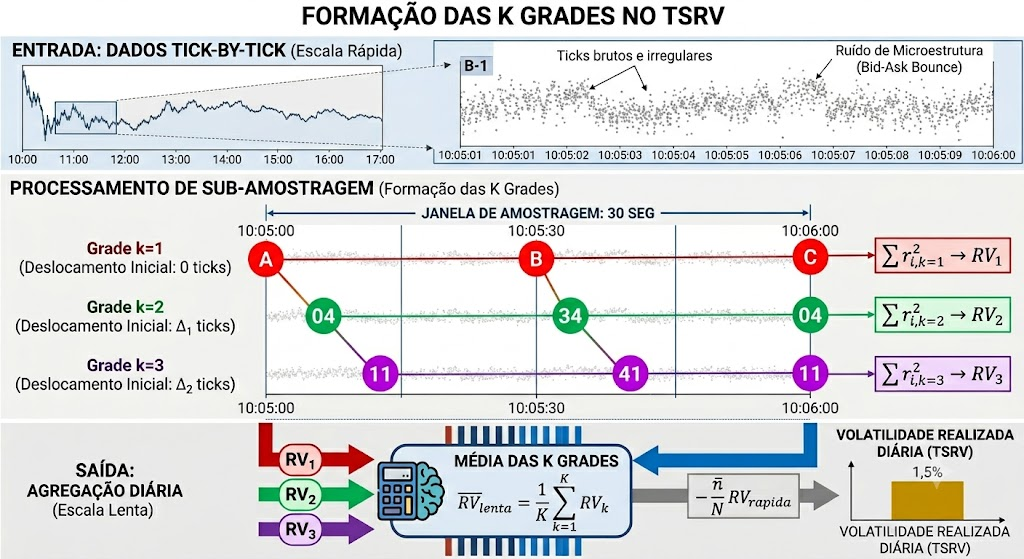
\includegraphics[width=0.95\textwidth]{TSRV_Ilustration.jpg}
	\caption{Ilustração para a estimação do TSRV.}
	\label{fig:ilustracao_tsrv}
\end{figure}

\subsubsection{Propriedades}

O estimador TSRV possui as seguintes propriedades \cite{zhang2005}:

\begin{enumerate}[label=\roman*)]
    \item \textbf{Consistência}: $\text{TSRV} \xrightarrow{p}
          \int_0^1 \sigma^2(t)\,dt$ quando $M \to \infty$, desde que
          $K = O(M^{2/3})$;
    \item \textbf{Taxa de convergência ótima}: sob a escolha
          $K = c \cdot M^{2/3}$ para uma constante $c > 0$ apropriada,
          o TSRV atinge a taxa de convergência
          $O_p(M^{-1/6})$, que é a minimax-ótima para estimação de
          volatilidade na presença de ruído;
    \item \textbf{Robustez ao ruído}: ao contrário da RV simples, o
          TSRV não diverge em frequências muito altas, podendo utilizar
          toda a informação intradiária disponível.
\end{enumerate}

Neste trabalho, a volatilidade realizada diária empregada como
\emph{benchmark} para avaliação dos modelos ARIMA-GARCH é calculada pelo
estimador TSRV a partir de dados \emph{tick-by-tick} do ativo, agregados em
diferentes frequências de amostragem (30 segundos, 1 minuto e 2 minutos).
A estimativa final (denominada \emph{RV consenso}) é obtida pela média das
três frequências, conferindo maior robustez ao \emph{benchmark}.

% ==========================================================
\section{Validação Cruzada Combinatória Purgada (CPCV)}
\label{sec:cpcv}
% ==========================================================

A avaliação de desempenho de modelos em séries temporais financeiras enfrenta
desafios específicos que invalidam a aplicação direta de técnicas padrão de
validação cruzada. A dependência temporal entre observações implica que a
separação aleatória entre conjuntos de treino e teste pode introduzir
vazamento de informação (\emph{information leakage}), conduzindo a
estimativas otimistas e não confiáveis do erro de
generalização \cite{lopez2018advances}.

A Validação Cruzada Combinatória Purgada (\emph{Combinatorial Purged
Cross-Validation} --- CPCV), proposta por
\citeonline{lopez2018advances}, endereça essas limitações por meio de três
mecanismos: (i) geração combinatória de múltiplas partições treino-teste,
(ii) purgação de observações sobrepostas e (iii) embargo temporal.

% ----------------------------------------------------------
\subsection{Formulação}
\label{subsec:cpcv_formulacao}
% ----------------------------------------------------------

Considere um conjunto de dados com $T$ observações ordenadas
cronologicamente. O procedimento CPCV opera da seguinte forma:

\begin{enumerate}
    \item \textbf{Particionamento}: o conjunto de dados é dividido em $N$
          grupos sequenciais e não-sobrepostos
          $G_1, G_2, \ldots, G_N$, cada um contendo aproximadamente
          $T/N$ observações;
    \item \textbf{Geração combinatória}: selecionam-se todas as
          combinações possíveis de $k$ grupos para compor o conjunto de
          teste, resultando em $\binom{N}{k}$ partições distintas de
          treino-teste. Os demais $N-k$ grupos formam o respectivo
          conjunto de treino;
    \item \textbf{Purgação (\emph{purging})}: para cada partição,
          removem-se do conjunto de treino as observações cujos rótulos
          (variáveis-resposta) apresentem sobreposição temporal com os
          rótulos do conjunto de teste, eliminando vazamento direto de
          informação;
    \item \textbf{Embargo}: adicionalmente, remove-se do conjunto de
          treino um número de observações imediatamente subsequentes ao
          final de cada bloco de teste, denominado período de embargo
          ($h$). Essa exclusão mitiga o vazamento indireto decorrente da
          correlação serial entre observações próximas.
\end{enumerate}

% ----------------------------------------------------------
\subsection{Número de Caminhos de Backtest}
\label{subsec:cpcv_caminhos}
% ----------------------------------------------------------

Uma propriedade fundamental do CPCV é a geração de múltiplos caminhos de
\emph{backtest} que cobrem toda a extensão temporal do conjunto de dados.
O número de caminhos distintos é dado
por \cite{lopez2018advances}:
%
\begin{equation}
    \label{eq:cpcv_paths}
    \varphi(N,k) = \binom{N}{k}\cdot\frac{k}{N}
    = \binom{N-1}{k-1}.
\end{equation}

Cada caminho corresponde a uma sequência cronológica completa de previsões
fora-da-amostra, permitindo a construção de uma distribuição empírica de
métricas de desempenho em vez de uma única estimativa pontual. 

% ==========================================================
\section{Métricas de Avaliação de Previsões de Volatilidade}
\label{sec:metricas}
% ==========================================================

A avaliação da qualidade de previsões de variância condicional requer
métricas que sejam robustas ao uso de \emph{proxies} ruidosos da
volatilidade verdadeira (latente). \citeonline{patton2011} demonstrou que
apenas determinadas funções de perda preservam o ordenamento correto de
modelos quando a variância realizada é utilizada como \emph{proxy}
imperfeito da volatilidade verdadeira. As métricas empregadas neste trabalho
pertencem a essa classe robusta e são complementadas pela regressão de
Mincer--Zarnowitz, pelo teste de Diebold--Mariano e por intervalos de
confiança \emph{bootstrap}.

Em todas as expressões a seguir, sejam $\hat{\sigma}_t^2$ a variância
condicional prevista pelo modelo e $\xi_t$ a volatilidade realizada (TSRV)
no dia $t$, para $t = 1, \ldots, T$.

% ----------------------------------------------------------
\subsection{Funções de Perda}
\label{subsec:funcoes_perda}
% ----------------------------------------------------------

\subsubsection{Erro Quadrático Médio (MSE)}

O Erro Quadrático Médio penaliza proporcionalmente ao quadrado do desvio
entre previsão e \emph{benchmark}:
%
\begin{equation}
    \label{eq:mse}
    \text{MSE} = \frac{1}{T}
    \sum_{t=1}^{T}
    \left(\hat{\sigma}_t^2 - \xi_t\right)^2.
\end{equation}
%
Por ser quadrática, a MSE atribui peso maior a erros de grande magnitude,
tornando-se sensível a episódios de volatilidade extrema. Pertence à classe
de funções de perda robustas de \citeonline{patton2011}, garantindo que o
\emph{ranking} de modelos é consistente mesmo quando $\xi_t$ é um
\emph{proxy} ruidoso.

\subsubsection{Erro Absoluto Médio (MAE)}

O Erro Absoluto Médio oferece uma medida mais robusta a \emph{outliers} do
que a MSE, pois penaliza linearmente os desvios:
%
\begin{equation}
    \label{eq:mae}
    \text{MAE} = \frac{1}{T}
    \sum_{t=1}^{T}
    \left|\hat{\sigma}_t^2 - \xi_t\right|.
\end{equation}

\subsubsection{Função de Perda QLIKE}

A função de perda \emph{quasi-likelihood} (QLIKE), proposta por
\citeonline{patton2011}, pertence à classe de funções de perda robustas e
penaliza assimetricamente sub e sobre-estimação:
%
\begin{equation}
    \label{eq:qlike}
    \text{QLIKE} = \frac{1}{T}
    \sum_{t=1}^{T}
    \left(\ln\hat{\sigma}_t^2 +
    \frac{\xi_t}{\hat{\sigma}_t^2}\right).
\end{equation}
%
A QLIKE é especialmente relevante porque seu \emph{ranking} de modelos é
preservado independentemente da \emph{proxy} utilizada, bastando que esta
seja proporcional à verdadeira variância. Valores mais negativos indicam
melhor aderência.

% ----------------------------------------------------------
\subsection{Regressão de Mincer--Zarnowitz}
\label{subsec:mincer_zarnowitz}
% ----------------------------------------------------------

A regressão de Mincer--Zarnowitz \cite{mincer1969} constitui um teste
clássico de avaliação de previsões. Estima-se por Mínimos Quadrados
Ordinários (MQO) a regressão:
%
\begin{equation}
    \label{eq:mz}
    \xi_t = \alpha + \beta\,\hat{\sigma}_t^2 + \varepsilon_t,
\end{equation}
%
onde $\varepsilon_t$ é o termo de erro. Sob a hipótese nula de que a
previsão é \textbf{ótima e não-viesada}, espera-se:
%
\begin{equation}
    \label{eq:mz_h0}
    H_0:\; \alpha = 0 \;\text{e}\; \beta = 1.
\end{equation}

O coeficiente $\alpha$ captura o viés sistemático da previsão:
$\alpha \neq 0$ indica que, em média, a previsão sobre ou subestima a
volatilidade realizada. O coeficiente $\beta$ mede a sensibilidade da
realização às previsões: $\beta < 1$ sugere atenuação (a previsão
sobreestima a amplitude das variações de volatilidade), enquanto $\beta > 1$
indica amplificação.

O \textbf{coeficiente de determinação} $R^2$ da regressão quantifica a
proporção da variação da volatilidade realizada explicada pelas previsões do
modelo, sendo interpretado como medida de poder preditivo. Um $R^2$ elevado
indica que o modelo captura satisfatoriamente a dinâmica temporal da
volatilidade.

% ----------------------------------------------------------
\subsection{Teste de Diebold--Mariano}
\label{subsec:diebold_mariano}
% ----------------------------------------------------------

O teste de \citeonline{diebold1995} permite comparar formalmente o poder
preditivo de dois modelos concorrentes. Sejam
$L_t^{(1)} = (\hat{\sigma}_{1,t}^2 - \xi_t)^2$ e
$L_t^{(2)} = (\hat{\sigma}_{2,t}^2 - \xi_t)^2$ as perdas (MSE) dos modelos
1 e 2, respectivamente. Define-se a diferença de perdas
$d_t = L_t^{(1)} - L_t^{(2)}$ e testa-se:
%
\begin{equation}
    \label{eq:dm_h0}
    H_0:\; \mathrm{E}[d_t] = 0
    \qquad\text{(igual poder preditivo).}
\end{equation}

A estatística de Diebold--Mariano é:
%
\begin{equation}
    \label{eq:dm_stat}
    \text{DM} = \frac{\bar{d}}{\sqrt{\widehat{\text{Var}}(\bar{d})}}
    \;\xrightarrow{d}\; \mathcal{N}(0, 1),
\end{equation}
%
onde $\bar{d} = T^{-1}\sum_{t=1}^T d_t$ e
$\widehat{\text{Var}}(\bar{d})$ é estimada com correção HAC
(\emph{Heteroskedasticity and Autocorrelation Consistent}) de
Newey--West para horizonte de previsão $h$. Um valor DM negativo e
estatisticamente significativo indica que o modelo 1 é superior; um valor
positivo e significativo indica superioridade do modelo 2.

% ----------------------------------------------------------
\subsection{Intervalos de Confiança Bootstrap}
\label{subsec:bootstrap_ic}
% ----------------------------------------------------------

Para construir intervalos de confiança para as métricas pontuais (MSE, MAE
e QLIKE), emprega-se o método de \textbf{bootstrap percentil
não-paramétrico} \cite{efron1993}. O procedimento consiste em:

\begin{enumerate}
    \item Formar $B$ reamostras de tamanho $T$ por sorteio com reposição dos
          pares $(\hat{\sigma}_t^2, \xi_t)$;
    \item Para cada reamostra $b = 1, \ldots, B$, calcular a métrica
          $\theta^{*}_b$;
    \item Obter o intervalo de confiança $(1-\alpha)$ pelos quantis da
          distribuição \emph{bootstrap}:
          %
          \begin{equation}
              \label{eq:bootstrap_ci}
              \text{IC}_{1-\alpha} = \left[
              \hat{\theta}^{*}_{\alpha/2},\;
              \hat{\theta}^{*}_{1-\alpha/2}\right],
          \end{equation}
          %
          onde $\hat{\theta}^{*}_{q}$ denota o quantil de ordem $q$ da
          distribuição de $\{\theta^{*}_b\}_{b=1}^{B}$.
\end{enumerate}

O \emph{bootstrap} percentil é preferível à inferência assintótica baseada
na distribuição normal neste contexto, pois as perdas de previsão de
volatilidade são tipicamente assimétricas e de cauda pesada, violando as
hipóteses de normalidade.
% ----------------------------------------------------------
% Capítulo 3 — Metodologia
% ----------------------------------------------------------
\chapter{Metodologia}
\label{cap:metodologia}

Este capítulo descreve os procedimentos empíricos adotados para investigar o
impacto do método de amostragem --- \emph{dollar bars} versus \emph{time
bars} --- sobre a qualidade preditiva de modelos ARMA-GARCH para a variância
condicional de retornos do par BTC/USDT. A exposição segue a ordem
cronológica da \emph{pipeline} de modelagem: coleta e preparação dos dados
(\autoref{sec:met_dados}), análise exploratória das séries
(\autoref{sec:met_exploratoria}), construção dos retornos
(\autoref{sec:met_retornos}), divisão treino-teste
(\autoref{sec:met_split}), seleção de parâmetros via CPCV
(\autoref{sec:met_cpcv}), estimação do modelo final
(\autoref{sec:met_estimacao}), agregação das previsões para nível diário
(\autoref{sec:met_agregacao}), avaliação por métricas e testes estatísticos
(\autoref{sec:met_metricas}) e implementação computacional
(\autoref{sec:met_implementacao}).

% ==========================================================
\section{Dados e Período Amostral}
\label{sec:met_dados}
% ==========================================================

O estudo utiliza dados de negociação do par BTC/USDT na \emph{exchange}
Binance, abrangendo o período de 1\textordmasculine\ de janeiro de 2024 a
31 de dezembro de 2025 (731 dias corridos). A partir dos dados brutos de
alta frequência, foram construídas duas séries de barras com resolução
efetiva equivalente a 5 minutos:

\begin{itemize}
    \item \textbf{Dollar Bars (5 min)}: 209.630 barras, amostradas sempre
          que o volume financeiro acumulado atinge um limiar
          $\bar{D}$ calibrado para produzir, em média, o mesmo número de
          barras por dia que as \emph{time bars} de 5 minutos;
    \item \textbf{Time Bars (5 min)}: 210.522 barras, amostradas em
          intervalos fixos de 5 minutos.
\end{itemize}

Adicionalmente, a volatilidade realizada diária, estimada pelo método
TSRV (\autoref{subsec:tsrv}), serve como \emph{benchmark} para avaliação
das previsões. O \emph{benchmark} cobre os mesmos 731 dias do período
amostral.

% ----------------------------------------------------------
\subsection{Coleta e Pré-processamento dos Dados de Alta Frequência}
\label{subsec:met_coleta}
% ----------------------------------------------------------

Os dados brutos utilizados neste trabalho consistem nos registros de negociação agregada (\emph{aggTrades}) do par BTC/USDT disponibilizados pela Binance. Cada observação contém o preço de execução da negociação, o volume transacionado e a direção do \emph{taker} (campo \texttt{IsBuyerMaker}). O volume total do período amostral supera 1 bilhão de registros, distribuídos em arquivos no formato Apache Parquet com tamanho agregado de aproximadamente 28\,GB.

Dado o volume de dados incompatível com o carregamento integral em memória principal (\emph{RAM}), adotou-se uma arquitetura de processamento por \emph{streaming}, descrita em detalhe a seguir.

\subsubsection{Arquitetura de Processamento por \emph{Streaming} via \emph{Row Groups}}
\label{subsubsec:streaming_rg}

O formato Parquet organiza os dados em unidades lógicas denominadas \emph{row groups} --- blocos contíguos de linhas armazenados de forma colunar. A biblioteca \texttt{pyarrow} permite a leitura seletiva de um \emph{row group} por vez, sem que o restante do arquivo seja desserializado. Essa característica foi explorada para implementar um laço de processamento iterativo: a cada iteração, um único \emph{row group} é carregado em memória, as métricas de microestrutura são calculadas e acumuladas em estruturas de dados de tamanho fixo, e o bloco é então descartado antes que o próximo seja lido.

O resultado prático é um consumo de memória aproximadamente constante ao longo de toda a execução --- empiricamente observado em torno de 500\,MB --- independentemente do tamanho total do arquivo. Tal abordagem é condição necessária para a replicabilidade do experimento em ambientes com recursos computacionais convencionais (ausência de infraestrutura de \emph{cluster}), garantindo ao mesmo tempo que a íntegra dos dados seja processada sem amostragem prévia.

\subsubsection{Extração do Preço Eficiente por Filtro IIR}
\label{subsubsec:filtro_iir}

No arcabouço de microestrutura, o preço observado $P_t$ é decomposto em duas componentes:
%
\begin{equation}
    \label{eq:price_decomp}
    P_t = P_t^* + \varepsilon_t,
\end{equation}
%
onde $P_t^*$ denota o \emph{preço eficiente} --- o valor fundamental latente do ativo, livre de ruído transacional --- e $\varepsilon_t$ representa o ruído de microestrutura, gerado pela discrição do \emph{tick}, pelo \emph{spread} \emph{bid-ask} e por outros custos de transação.

Para extrair $P_t^*$, aplicou-se um filtro de Média Móvel Exponencial (EMA) de primeira ordem, equivalente a um filtro de Resposta ao Impulso Infinita (IIR) passa-baixas com função de transferência:
%
\begin{equation}
    \label{eq:iir}
    H(z) = \frac{\alpha}{1 - (1-\alpha)\,z^{-1}},
\end{equation}
%
onde $\alpha \in (0,1)$ é o coeficiente de suavização. A equação de recorrência correspondente é $P_t^* = \alpha P_t + (1-\alpha)P_{t-1}^*$, que pode ser implementada de forma causal e eficiente via \texttt{scipy.signal.lfilter}. A denominação ``IIR'' sublinha que, ao contrário dos filtros de Resposta ao Impulso Finita (FIR), cada saída depende de toda a história passada da série, tornando a manutenção do \emph{estado} do filtro entre os \emph{row groups} processados indispensável para garantir a continuidade do sinal: ao final de cada bloco, o vetor de estado interno do filtro é preservado e injetado como condição inicial do bloco subsequente.

O componente de ruído é então estimado como o resíduo $\hat{\varepsilon}_t = P_t - \hat{P}_t^*$, e suas propriedades estatísticas --- média, variância, percentis e perfil intradiário --- são acumuladas nas estruturas \emph{online} descritas nas subseções anteriores.

\subsubsection{Aceleração por Compilação JIT via Numba}
\label{subsubsec:numba}

Os \emph{kernels} de cálculo que envolvem laços internos sobre janelas móveis --- em particular, o estimador de Hasbrouck e a covariância serial do modelo de Roll --- foram decorados com a diretiva \texttt{@numba.njit} (modo \emph{nopython}), que instrui o compilador Numba a traduzir o código Python para código de máquina LLVM sem intermediação do interpretador CPython. O resultado é desempenho equivalente ao de C para laços numéricos intensivos, com o benefício de manter a legibilidade e a verificabilidade do código em Python. O ganho de velocidade observado em relação ao NumPy puro para janelas de comprimento $\sim$$10^4$ foi superior a uma ordem de grandeza, tornando o processamento da série completa viável em tempo compatível com o ciclo de pesquisa.

% ----------------------------------------------------------
\subsection{Estimação da Volatilidade Realizada}
\label{subsec:met_rv_estimacao}
% ----------------------------------------------------------

A Volatilidade Realizada (RV) é uma medida não paramétrica da variância integrada de um processo de preços, obtida pela soma dos quadrados dos log-retornos observados em alta frequência \cite{andersen2003}. Para um ativo com preços $P_0, P_1, \ldots, P_n$ amostrados a intervalos regulares, o estimador clássico é definido como:
%
\begin{equation}
    \label{eq:rv_classica}
    \widehat{RV}_n = \sum_{i=1}^{n} r_i^2,
    \qquad r_i = \ln\!\left(\frac{P_i}{P_{i-1}}\right).
\end{equation}
%
Sob o modelo de difusão sem ruído, $\widehat{RV}_n$ converge em probabilidade para a variância integrada $\int_0^1 \sigma_s^2\,\mathrm{d}s$ quando $n \to \infty$. No entanto, dados de altíssima frequência como \emph{aggTrades} da Binance são contaminados por ruído de microestrutura de mercado --- originado pelo \emph{bid-ask bounce}, pela discrição do \emph{tick} e por custos de transação ---, o que induz viés crescente em $\widehat{RV}_n$ à medida que a frequência de amostragem aumenta. Esse fenômeno é denominado o \emph{bias-variance trade-off} da volatilidade realizada.

% ----------------------------------------------------------
\subsubsection{Two-Scale Realized Volatility (TSRV)}
\label{subsec:tsrv}
% ----------------------------------------------------------

Para contornar o viés imposto pelo ruído de microestrutura, adotou-se o estimador \emph{Two-Scale Realized Volatility} (TSRV), proposto por \citeonline{zhang2005}. A ideia central é combinar duas escalas de observação: uma escala ``grossa'' (sub-grids), menos suscetível ao ruído, e a escala completa, que serve de base para a correção do viés.

Sejam $n$ log-retornos calculados sobre preços amostrados a uma frequência regular. O estimador TSRV é construído em três etapas:

\begin{enumerate}
    \item \textbf{RV na escala completa.} Calcula-se a RV clássica sobre todos os $n$ retornos:
    %
    \begin{equation}
        \label{eq:rv_all}
        \widehat{RV}^{(\text{all})} = \sum_{i=1}^{n} r_i^2.
    \end{equation}

    \item \textbf{Divisão em $K$ sub-grids e RV média.} Os índices $\{1, \ldots, n\}$ são particionados em $K$ sub-grids, onde o sub-grid $k$ contém os índices $\{k, k+K, k+2K, \ldots\}$. Para cada sub-grid $k$, calcula-se a RV parcial $\widehat{RV}^{(k)}$ a partir dos retornos entre observações consecutivas dentro do sub-grid. A média das $K$ RVs parciais fornece:
    %
    \begin{equation}
        \label{eq:rv_subgrid}
        \overline{RV}^{(K)} = \frac{1}{K}\sum_{k=1}^{K} \widehat{RV}^{(k)}.
    \end{equation}

    \item \textbf{Correção de viés.} O estimador TSRV corrige o viés de ruído subtraindo uma fração da RV na escala completa:
    %
    \begin{equation}
        \label{eq:tsrv}
        \widehat{TSRV} = \overline{RV}^{(K)} - \frac{\bar{n}}{n}\,\widehat{RV}^{(\text{all})},
    \end{equation}
    %
    onde $\bar{n} = n/K$ é o tamanho médio de cada sub-grid. A intuição é que o termo $(\bar{n}/n)\,\widehat{RV}^{(\text{all})}$ estima a contribuição do ruído à RV na escala completa, que é proporcional ao número de observações.
\end{enumerate}

\textbf{Determinação do $K$ ótimo.} \citeonline{zhang2005} demonstram que o $K$ que minimiza o erro quadrático médio assintótico do estimador é:
%
\begin{equation}
    \label{eq:k_otimo}
    K^* = \left\lfloor n^{2/3} \right\rceil,
\end{equation}
%
onde $\lfloor\cdot\rceil$ denota o arredondamento para o inteiro mais próximo. Na implementação, $K$ é limitado superiormente por $\lfloor n/2 \rfloor$ para garantir que cada sub-grid contenha ao menos duas observações. O estimador final é truncado em zero ($\max(\widehat{TSRV},\,0)$) para garantir não-negatividade em amostras finitas.

% ----------------------------------------------------------
\subsubsection{Amostragem em Tempo Calendário}
\label{subsubsec:amostragem_calendario}
% ----------------------------------------------------------

Os \emph{ticks} brutos chegam em tempo de transação irregular, tornando necessária uma reestruturação temporal antes do cômputo da TSRV. Adotou-se a amostragem em tempo calendário (\emph{calendar-time sampling}): para cada frequência $\Delta$ configurável (ex.: 30s, 1 min, 2 min), o preço correspondente a cada intervalo $[t, t+\Delta)$ é definido como o preço da \emph{última} transação executada naquele intervalo (\texttt{resample($\Delta$).last()}). Intervalos sem negociação são descartados (\texttt{dropna()}). Esse procedimento produz uma grade temporal regular de preços $P_1, P_2, \ldots, P_n$ sobre a qual os log-retornos são calculados via diferenciação logarítmica: $r_i = \ln(P_i) - \ln(P_{i-1})$.

% ----------------------------------------------------------
\subsubsection{Processamento Diário Eficiente (\texttt{TickDataProcessor})}
\label{subsubsec:tick_processor}
% ----------------------------------------------------------

Dado o volume de dados (superior a 1 bilhão de registros), o processamento é realizado dia a dia. A classe \texttt{TickDataProcessor} encapsula a leitura seletiva de dados do arquivo Parquet via filtros aplicados diretamente no disco (\texttt{pyarrow.parquet.read\_parquet} com predicado de intervalo de datas), carregando em memória apenas as colunas \texttt{DateTime}, \texttt{Price} e \texttt{Qty} referentes a um único dia de negociação. Para cada dia, a função \texttt{compute\_daily\_rv} realiza: (i) a reestruturação temporal por reamostragem; (ii) a instanciação da classe \texttt{TwoScaleRV} sobre o vetor de preços resultante; e (iii) o cômputo do estimador com coleta de estatísticas auxiliares --- número de \emph{ticks}, número de observações amostradas, volume financeiro e preço médio.

% ----------------------------------------------------------
\subsubsection{Benchmark de Consenso Multi-Frequência}
\label{subsubsec:benchmark_consenso}
% ----------------------------------------------------------

A escolha da frequência de reamostragem $\Delta$ introduz um grau de arbitrariedade nas estimativas de TSRV. Para mitigar esse efeito, construiu-se um \emph{benchmark} de consenso: a \emph{pipeline} \texttt{compute\_rv\_series} é executada independentemente para três frequências --- 30 segundos, 1 minuto e 2 minutos --- gerando três séries diárias de RV, denotadas $\widehat{TSRV}_{30\text{s},d}$, $\widehat{TSRV}_{1\text{min},d}$ e $\widehat{TSRV}_{2\text{min},d}$. O benchmark de consenso para o dia $d$ é então definido como a média aritmética dessas três estimativas:
%
\begin{equation}
    \label{eq:rv_consenso}
    \widehat{RV}_{\text{consenso},d} = \frac{1}{3}\!\left(\widehat{TSRV}_{30\text{s},d} + \widehat{TSRV}_{1\text{min},d} + \widehat{TSRV}_{2\text{min},d}\right),
\end{equation}
%
com dias em que qualquer das três frequências produziu valor ausente (\texttt{NaN}) tratados de forma robusta pela média sobre os valores disponíveis. Essa abordagem reduz a sensibilidade do benchmark a escolhas arbitrárias de $\Delta$ e fornece uma medida mais estável da variância integrada diária.

A volatilidade anualizada correspondente é obtida por:
%
\begin{equation}
    \label{eq:vol_anualizada}
    \hat{\sigma}_{\text{anual},d} = \sqrt{\widehat{RV}_{\text{consenso},d} \times 252}.
\end{equation}

% ==========================================================
\section{Análise Exploratória das Séries}
\label{sec:met_exploratoria}
% ==========================================================

Antes de proceder à modelagem, realizou-se uma análise exploratória das
séries completas de retornos logarítmicos, com o objetivo de verificar as
premissas dos modelos ARMA-GARCH e identificar diferenças distribucional
e de dependência entre os dois métodos de amostragem.

% ----------------------------------------------------------
\subsection{Estatísticas Descritivas}
\label{subsec:met_descritivas}
% ----------------------------------------------------------

A \autoref{tab:descritivas} apresenta os quatro primeiros momentos
amostrais da distribuição dos retornos para ambos os tipos de barra. As
estatísticas foram calculadas sobre a série completa (209.630 observações
para \emph{dollar bars} e 210.522 para \emph{time bars}).

\begin{table}[H]
\centering
\caption{Estatísticas descritivas dos retornos logarítmicos.}
\label{tab:descritivas}
\begin{tabular}{lSS}
\toprule
{Estatística} & {\emph{Dollar Bars}} & {\emph{Time Bars}} \\
\midrule
Média ($1^{\circ}$ momento)        &  3.46e-6  &  3.44e-6  \\
Variância ($2^{\circ}$ momento)    &  2.49e-6  &  2.40e-6  \\
Assimetria ($3^{\circ}$ momento)   &  0.0547   & -1.0071   \\
Curtose de Fisher ($4^{\circ}$ momento) &  3.0879   &  75.3687  \\
\bottomrule
\end{tabular}
\fonte{Elaboração própria.}
\end{table}

Dois aspectos merecem destaque. Primeiro, ambas as séries apresentam
excesso de curtose positivo, indicando caudas mais pesadas do que a
distribuição normal --- um fato estilizado amplamente documentado em
retornos financeiros \cite{tsay2010}. Entretanto, a magnitude do excesso
de curtose é drasticamente diferente: enquanto os retornos de
\emph{dollar bars} exibem curtose de Fisher igual a 3,09, os retornos de
\emph{time bars} alcançam 75,37, evidenciando a presença de observações
extremas significativamente mais severas.

Segundo, a assimetria dos retornos de \emph{time bars} ($-1,01$) é
substancialmente mais negativa do que a dos \emph{dollar bars} ($0,05$,
praticamente simétrica). Isso sugere que a amostragem temporal fixa
captura eventos de cauda esquerda (quedas abruptas) de forma mais
concentrada, possivelmente por comprimir muitas transações em uma única
barra durante episódios de alta volatilidade.

Esses resultados corroboram a tese de
\citeonline{lopez2018advances}: \emph{dollar bars} produzem retornos
com propriedades distribucional mais favoráveis à modelagem estatística.

% ----------------------------------------------------------
\subsection{Testes de Normalidade, Estacionariedade e Heteroscedasticidade}
\label{subsec:met_testes}
% ----------------------------------------------------------

A \autoref{tab:testes} sintetiza os resultados dos testes aplicados.

\begin{table}[H]
\centering
\caption{Testes de normalidade, estacionariedade e
heteroscedasticidade sobre os retornos logarítmicos.}
\label{tab:testes}
\begin{tabular}{lSSSS}
\toprule
{Teste} &
\multicolumn{2}{c}{\emph{Dollar Bars}} &
\multicolumn{2}{c}{\emph{Time Bars}} \\
\cmidrule(lr){2-3} \cmidrule(lr){4-5}
& {Estat.} & {\emph{p}-valor} & {Estat.} & {\emph{p}-valor} \\
\midrule
Jarque-Bera          & 83384.65  & {$<0{,}001$} & 49860565.37 & {$<0{,}001$} \\
Kolmogorov-Smirnov   & 0.0123    & {$<0{,}001$} & 0.0934      & {$<0{,}001$} \\
\addlinespace
ADF                  & -102.46   & {$<0{,}001$} & -57.32      & {$<0{,}001$} \\
KPSS                 & 0.2053    & 0.10         & 0.2171      & 0.10         \\
\addlinespace
Ljung-Box ($r_t$, lag 10)   & 50.06    & {$<0{,}001$} & 155.03   & {$<0{,}001$} \\
Ljung-Box ($r_t^2$, lag 10) & 79528.20 & {$<0{,}001$} & 28237.22 & {$<0{,}001$} \\
ARCH de Engle (lag 10)      & 30420.71 & {$<0{,}001$} & 24064.78 & {$<0{,}001$} \\
\bottomrule
\end{tabular}
\nota{H$_0$ por teste: Jarque-Bera e KS — normalidade;
ADF — raiz unitária; KPSS — estacionariedade;
Ljung-Box e ARCH de Engle — ausência de autocorrelação/efeito ARCH.}
\fonte{Elaboração própria.}
\end{table}

Os resultados permitem extrair três conclusões:

\begin{enumerate}
    \item \textbf{Não-normalidade}: ambos os testes de normalidade
          (Jarque-Bera e Kolmogorov-Smirnov) rejeitam a hipótese nula a
          qualquer nível de significância convencional ($p < 0{,}001$), confirmando
          que os retornos não seguem distribuição gaussiana. Nota-se que a
          estatística de Jarque-Bera para \emph{time bars} é mais de 500
          vezes maior do que para \emph{dollar bars}, refletindo a curtose
          extrema da amostragem temporal;
    \item \textbf{Estacionariedade}: o teste ADF rejeita a hipótese nula
          de raiz unitária para ambas as séries ($p < 0{,}001$), enquanto o
          teste KPSS \emph{não} rejeita a hipótese nula de estacionariedade
          ($p = 0{,}10$). Os dois testes são consistentes e confirmam que as
          séries de retornos são estacionárias, não sendo necessária
          diferenciação ($d = 0$);
    \item \textbf{Efeitos ARCH}: tanto o teste de Ljung-Box sobre os
          retornos quadráticos quanto o teste ARCH de Engle rejeitam
          fortemente a hipótese nula de ausência de heteroscedasticidade
          condicional ($p < 0{,}001$), justificando a utilização de modelos
          da família GARCH para capturar a dinâmica da variância
          condicional.
\end{enumerate}

Adicionalmente, a \autoref{fig:normalidade_dollar} e a
\autoref{fig:normalidade_time} apresentam os histogramas com curva normal
ajustada e os QQ-plots dos retornos para cada tipo de barra, ilustrando
visualmente o afastamento da normalidade.

\begin{figure}[H]
    \centering
    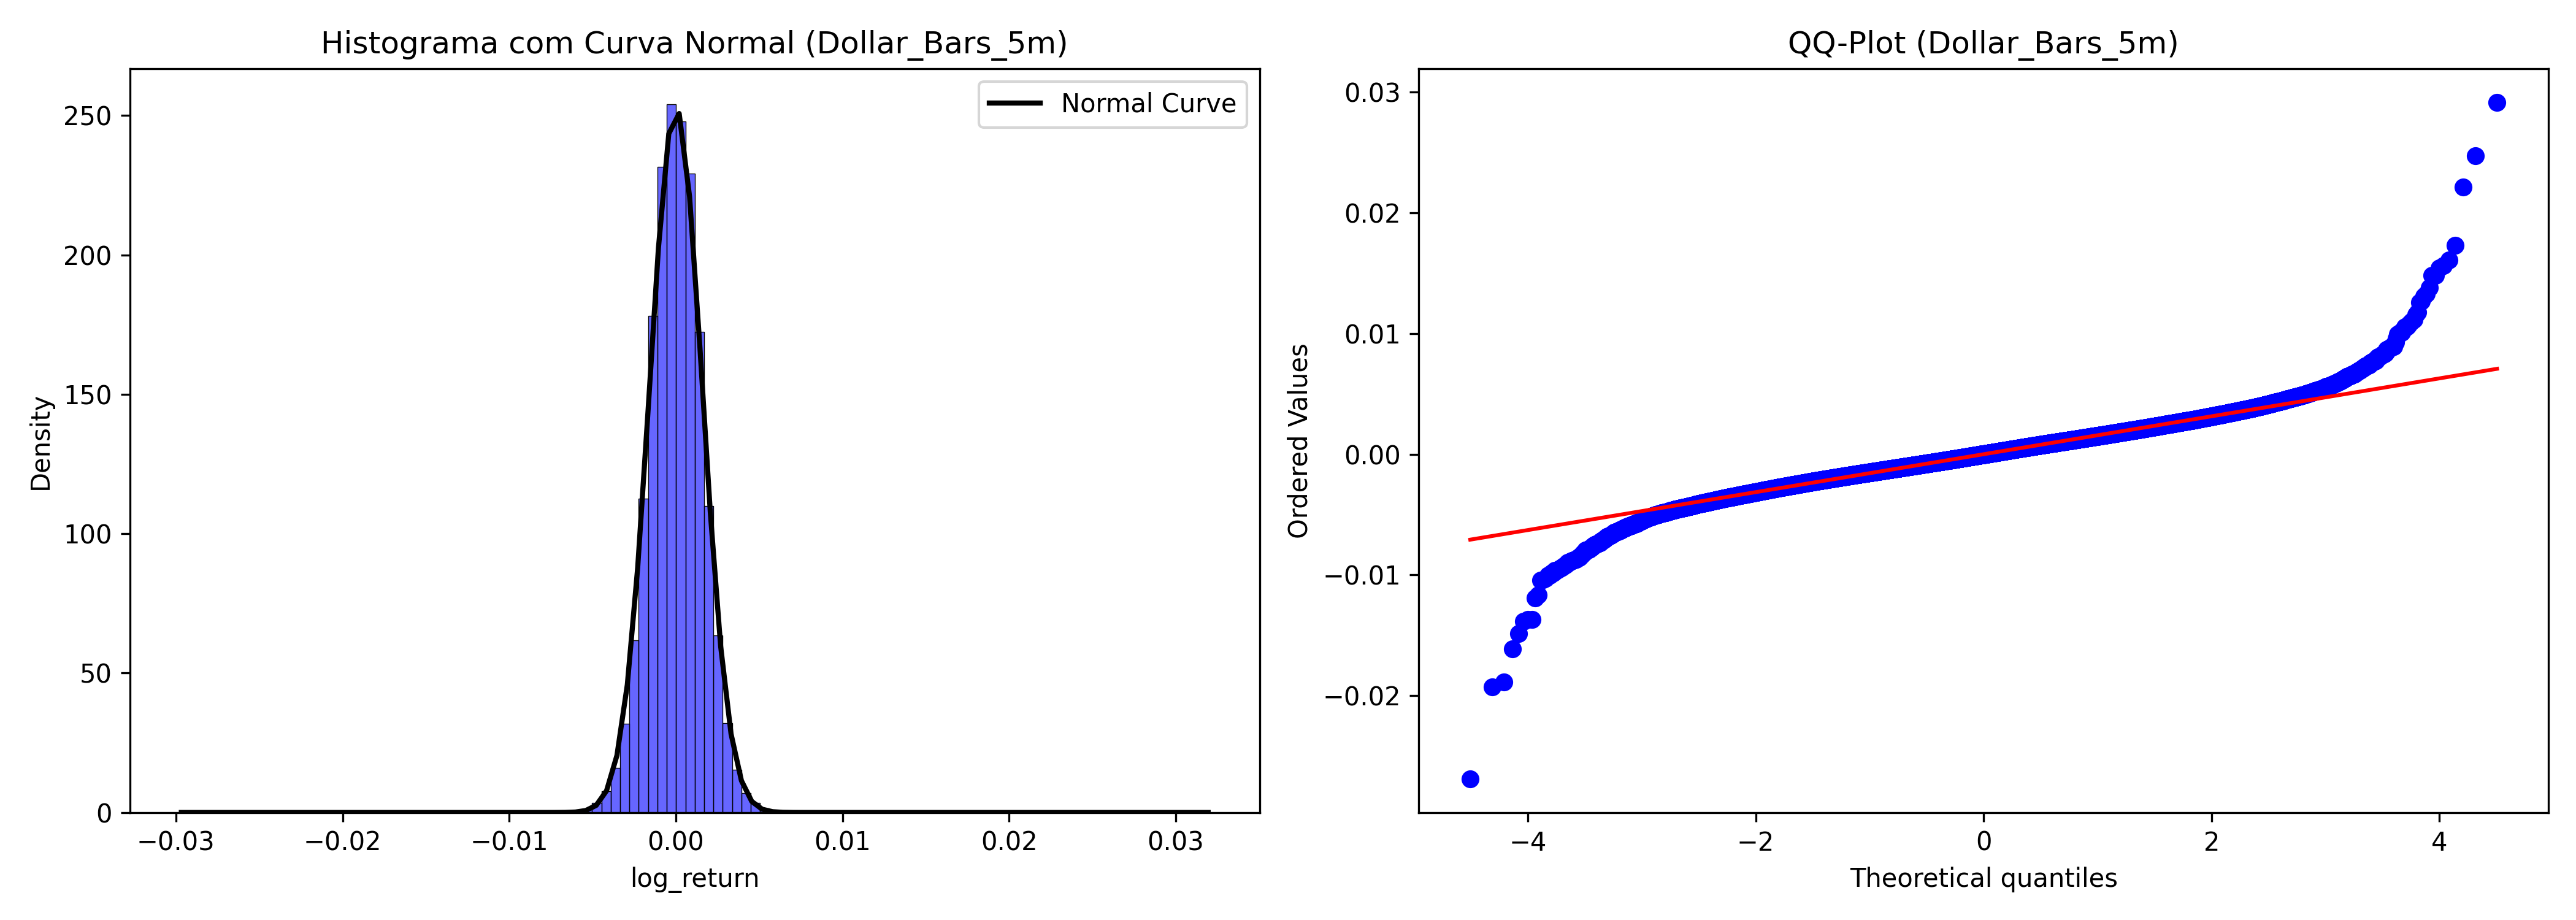
\includegraphics[width=0.95\textwidth]{Dollar_Bars_5m_normalidade.png}
    \caption{Histograma com curva normal e QQ-Plot --- Dollar Bars (5 min).}
    \label{fig:normalidade_dollar}
\end{figure}

\begin{figure}[H]
    \centering
    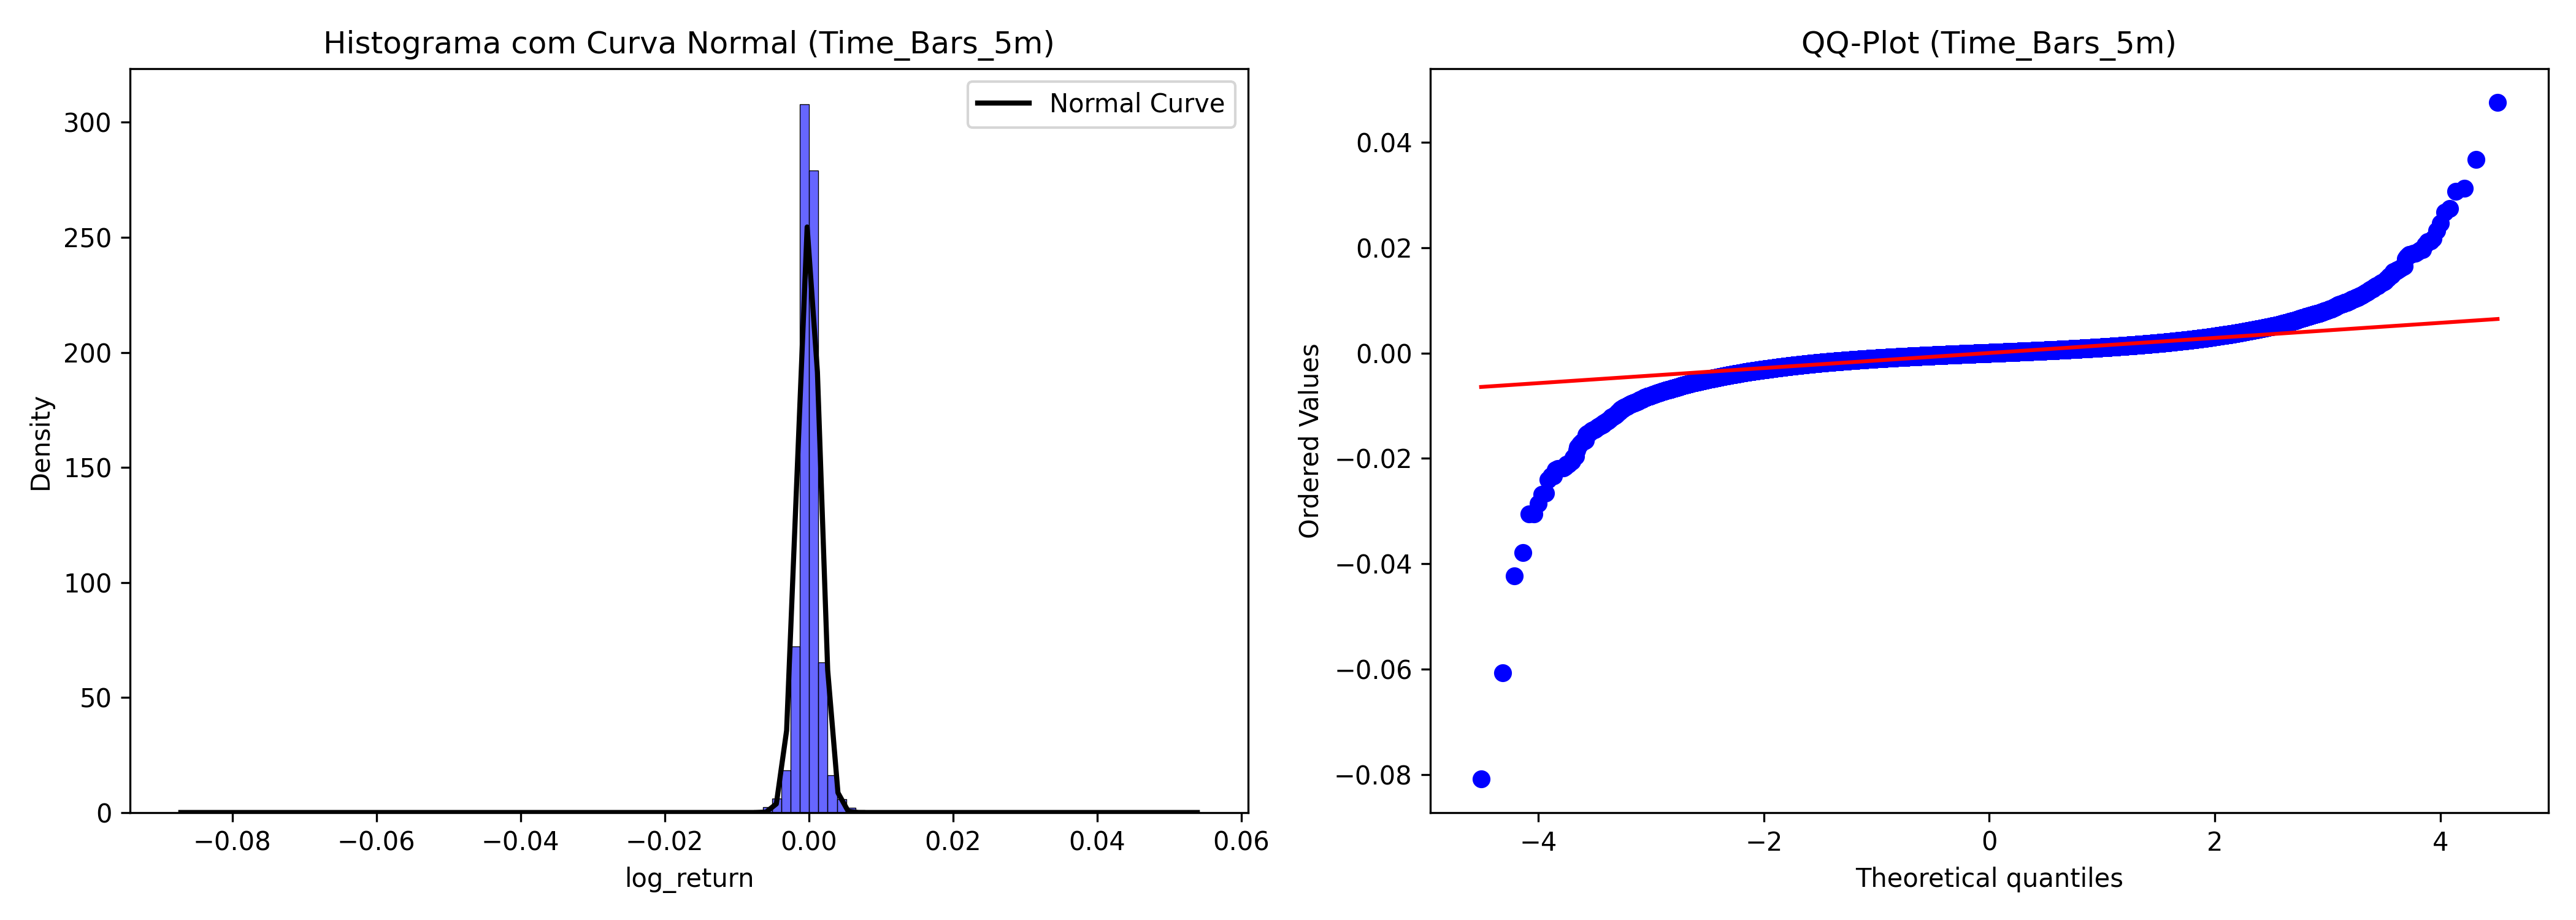
\includegraphics[width=0.95\textwidth]{Time_Bars_5m_normalidade.png}
    \caption{Histograma com curva normal e QQ-Plot --- Time Bars (5 min).}
    \label{fig:normalidade_time}
\end{figure}

A \autoref{fig:acf_dollar_sq} e a \autoref{fig:acf_time_sq} apresentam as
funções de autocorrelação (FAC) e autocorrelação parcial (FACP) dos
retornos ao quadrado, evidenciando a persistência da volatilidade
condicional em ambas as séries.

\begin{figure}[H]
    \centering
    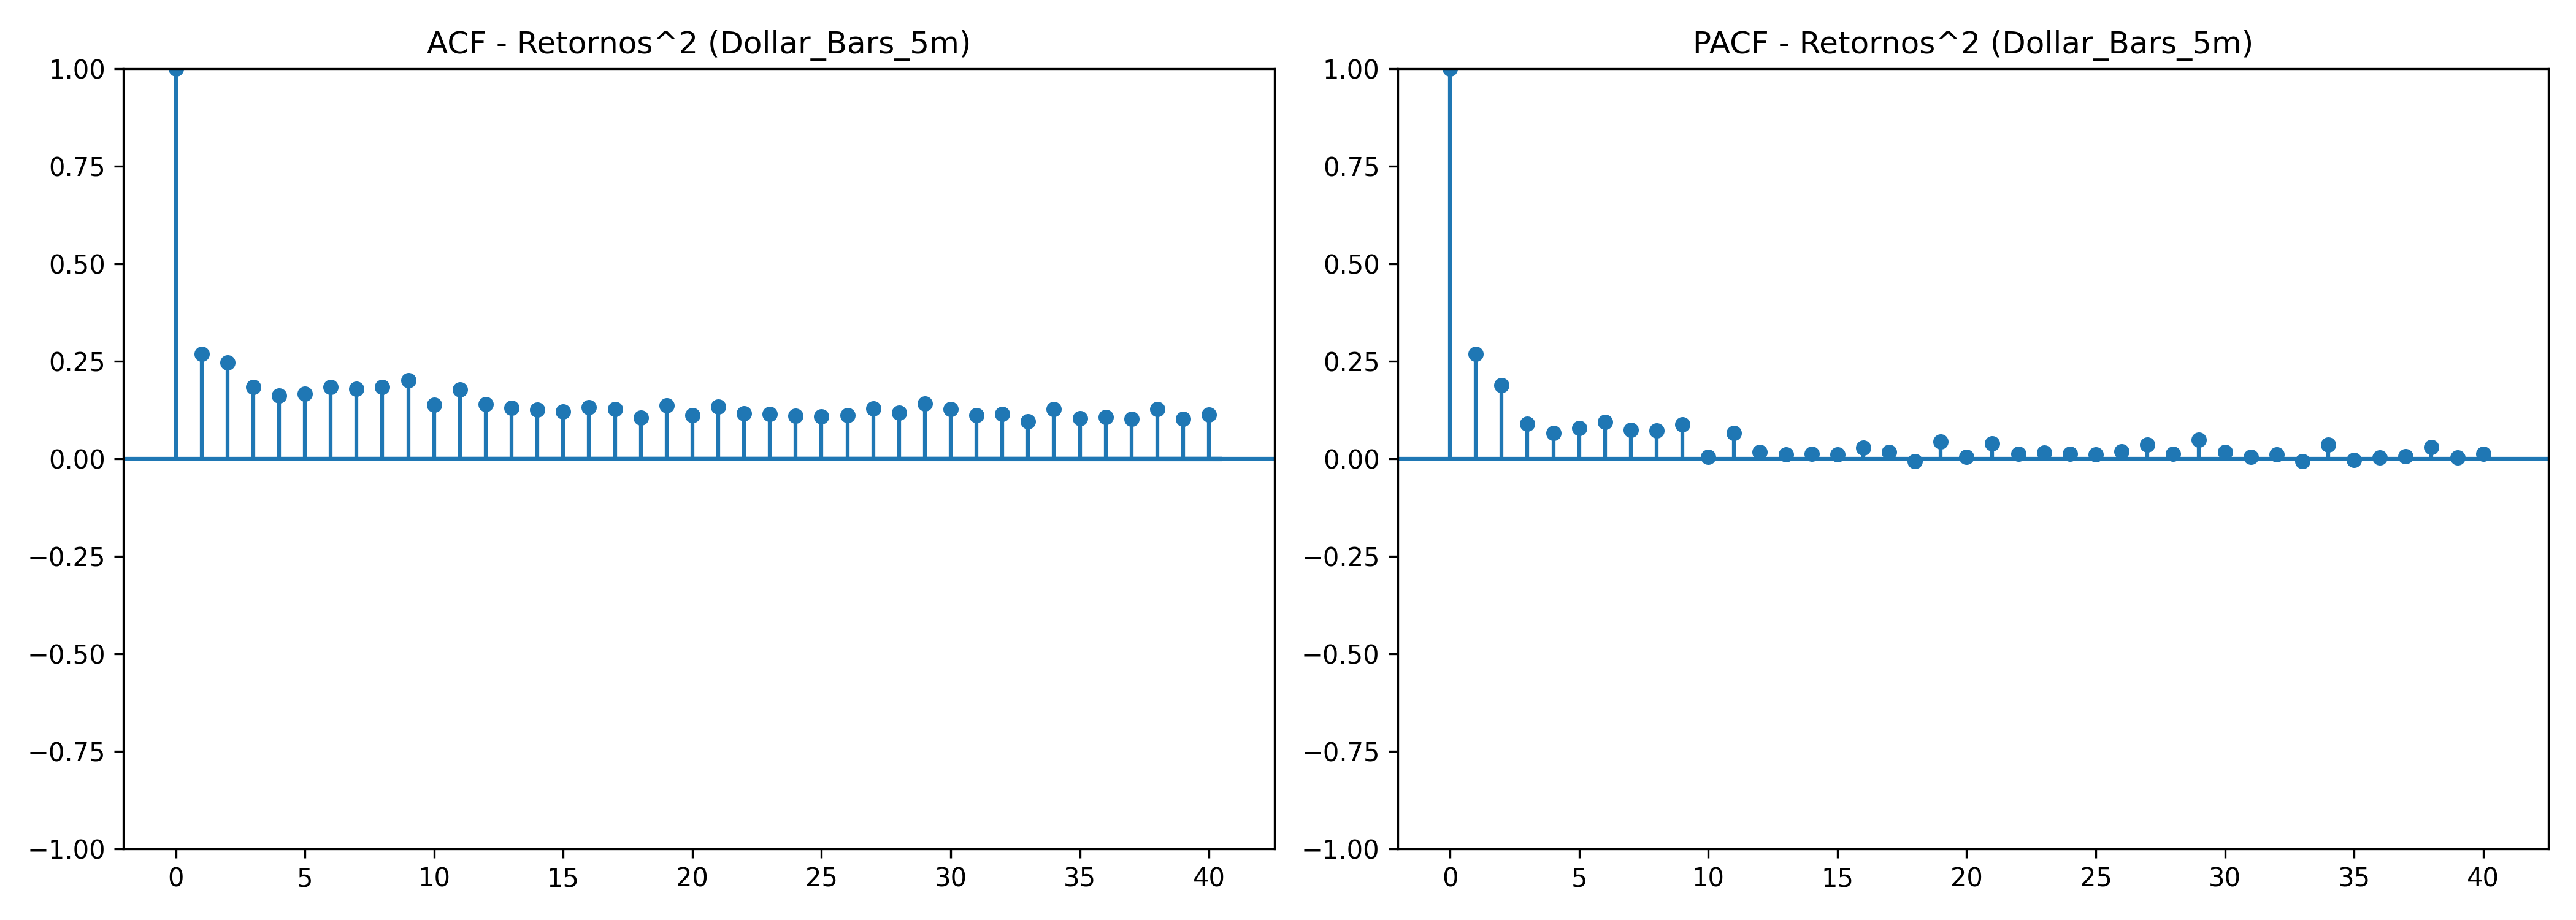
\includegraphics[width=0.95\textwidth]{Dollar_Bars_5m_acf_pacf_retornos2.png}
    \caption{ACF e PACF dos retornos ao quadrado --- Dollar Bars (5 min).}
    \label{fig:acf_dollar_sq}
\end{figure}

\begin{figure}[H]
    \centering
    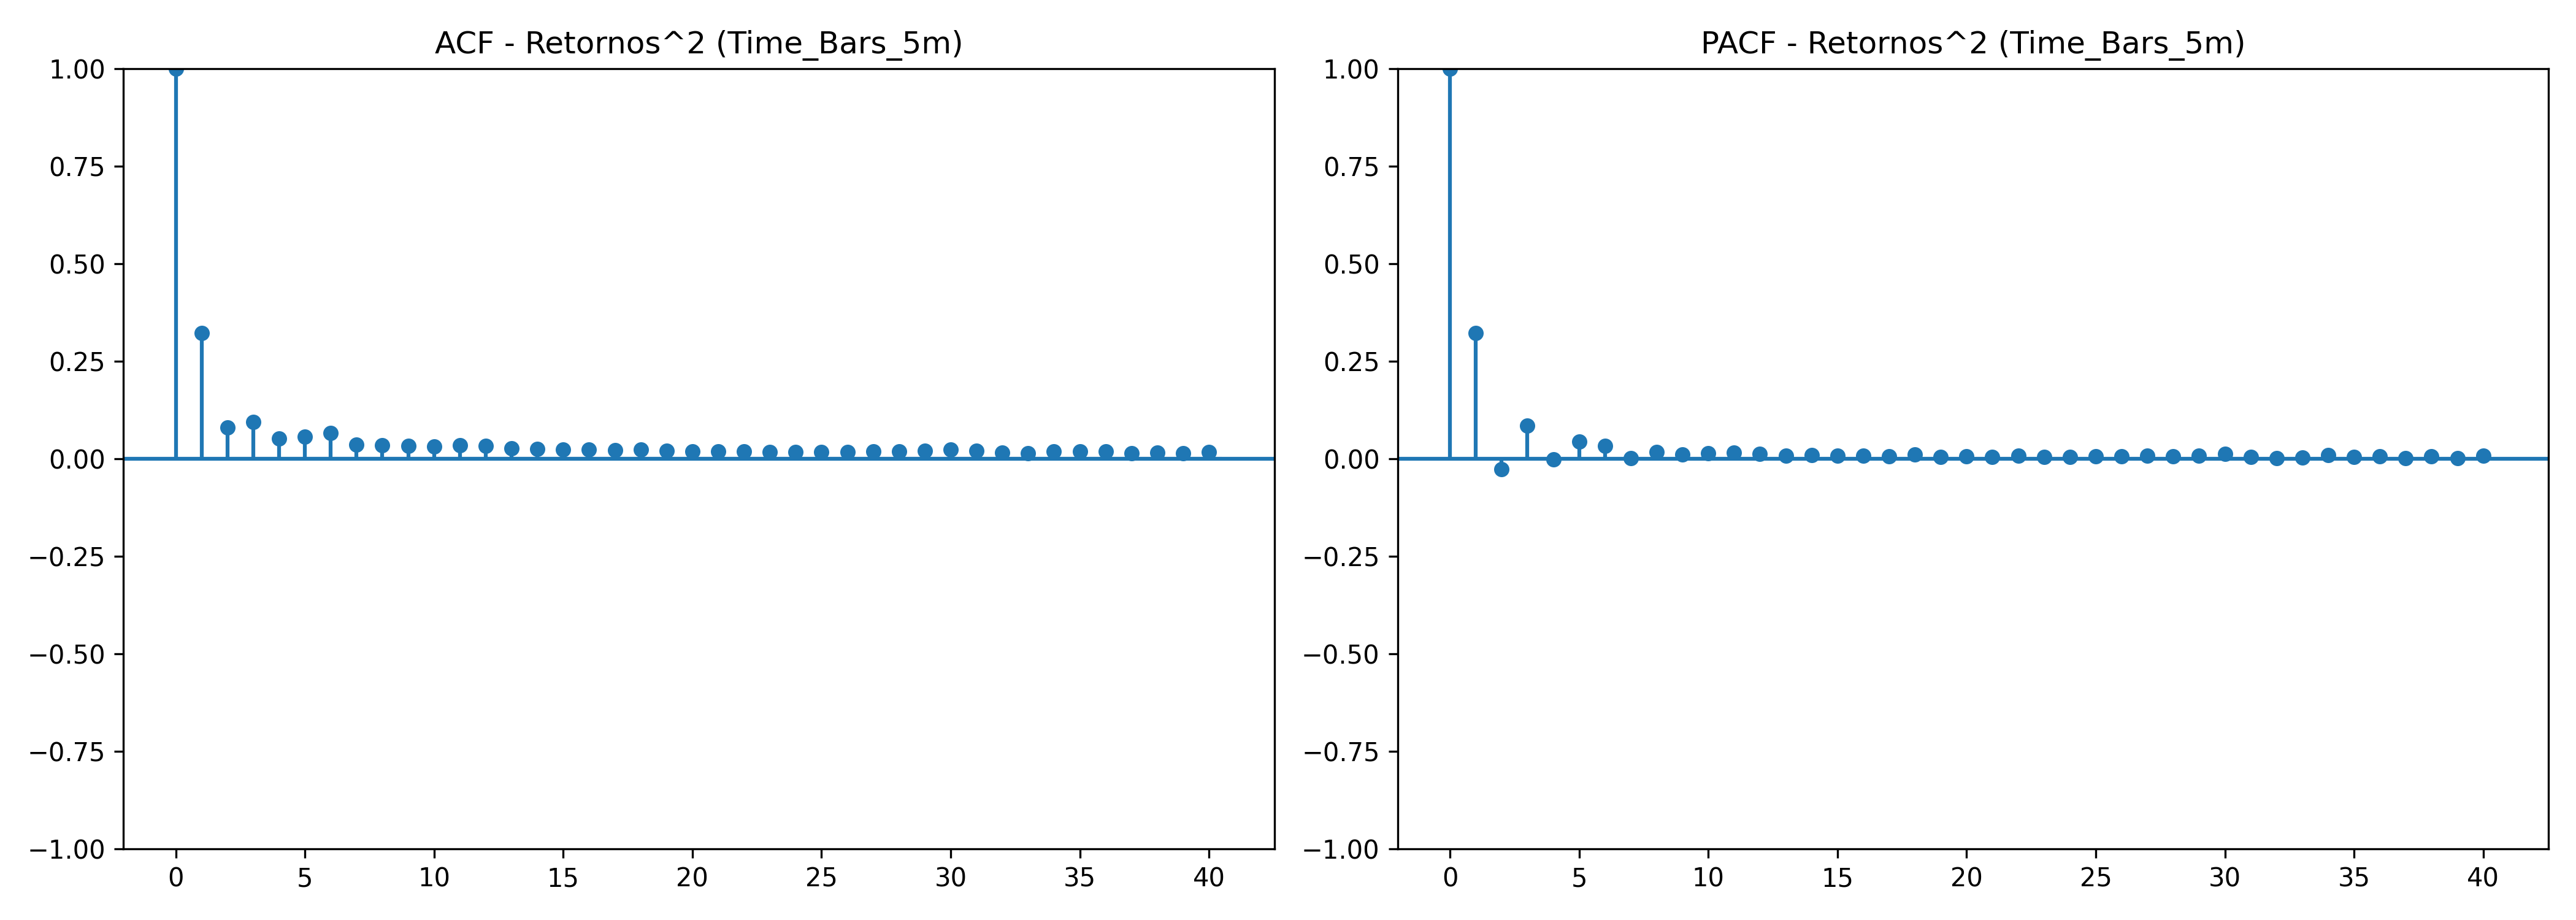
\includegraphics[width=0.95\textwidth]{Time_Bars_5m_acf_pacf_retornos2.png}
    \caption{ACF e PACF dos retornos ao quadrado --- Time Bars (5 min).}
    \label{fig:acf_time_sq}
\end{figure}

% ==========================================================
\section{Construção dos Retornos Logarítmicos}
\label{sec:met_retornos}
% ==========================================================

Para cada série de barras, os retornos logarítmicos foram calculados como:
%
\begin{equation}
    \label{eq:met_log_return}
    r_t = \ln\left(\frac{C_t}{C_{t-1}}\right),
\end{equation}
%
onde $C_t$ denota o preço de fechamento da $t$-ésima barra. A primeira
observação de cada série é descartada ($r_1$ é indefinido), resultando em
209.629 retornos para \emph{dollar bars} e 210.521 para \emph{time bars}.

A opção por retornos logarítmicos em vez de retornos simples
($R_t = C_t/C_{t-1} - 1$) justifica-se por duas razões: (i)~retornos
logarítmicos são aditivos ao longo do tempo, facilitando a agregação
temporal de variâncias; e (ii)~para retornos de pequena magnitude, como é
o caso de barras de 5 minutos, $r_t \approx R_t$, de modo que a escolha é
praticamente irrelevante numericamente.

% ==========================================================
\section{Divisão Treino-Teste}
\label{sec:met_split}
% ==========================================================

A amostra total de cada série foi dividida em dois conjuntos por meio de um
\emph{split} temporal na proporção 80\%/20\%, preservando a ordem
cronológica dos dados. A \autoref{tab:split} resume as dimensões e períodos
de cada partição.

\begin{table}[H]
\centering
\caption{Divisão treino-teste por tipo de barra.}
\label{tab:split}
\begin{tabular}{llrr}
\toprule
{Série} & {Partição} & {Observações} & {Período} \\
\midrule
\multirow{2}{*}{\emph{Dollar Bars}}
    & Treino (80\%) & 167.704 & 01/jan/2024 -- 14/jul/2025 \\
    & Teste (20\%)  &  41.926 & 14/jul/2025 -- 31/dez/2025 \\
\addlinespace
\multirow{2}{*}{\emph{Time Bars}}
    & Treino (80\%) & 168.417 & 01/jan/2024 -- 07/ago/2025 \\
    & Teste (20\%)  &  42.105 & 07/ago/2025 -- 31/dez/2025 \\
\bottomrule
\end{tabular}
\fonte{Elaboração própria.}
\end{table}

Observa-se que as datas de corte diferem ligeiramente entre os dois tipos
de barra (14 de julho vs. 7 de agosto de 2025), uma vez que a proporção
80\%/20\% é definida sobre o número de barras, e não sobre o calendário.
Isso é esperado, pois as \emph{dollar bars} possuem espaçamento temporal
irregular.

É importante ressaltar que a divisão treino-teste é distinta do
procedimento de validação cruzada CPCV descrito na
\autoref{sec:met_cpcv}: o CPCV opera exclusivamente sobre o conjunto de
\textbf{treino} para selecionar os hiperparâmetros, enquanto o conjunto de
\textbf{teste} é reservado para a avaliação final do modelo selecionado.

% ==========================================================
\section{Seleção de Parâmetros via CPCV}
\label{sec:met_cpcv}
% ==========================================================

A seleção das ordens ótimas $(p, q)$ para a equação da média
(ARMA) e $(r, s)$ para a equação da variância (GARCH) foi realizada pelo
arcabouço de Validação Cruzada Combinatória Purgada (CPCV), descrito na
\autoref{sec:cpcv}. Este procedimento foi aplicado exclusivamente ao
conjunto de treino de cada série.

% ----------------------------------------------------------
\subsection{Configuração do CPCV}
\label{subsec:met_cpcv_config}
% ----------------------------------------------------------

O CPCV foi configurado com os seguintes parâmetros:

\begin{itemize}
    \item \textbf{Número de grupos}: $N = 10$ (o conjunto de treino é
          dividido em 10 blocos sequenciais);
    \item \textbf{Grupos de teste}: $k = 5$ (a cada partição, 5 grupos
          compõem o teste);
    \item \textbf{Número de folds}: $\binom{10}{5} = 252$ partições
          treino-teste distintas;
    \item \textbf{Embargo}: 240 barras ($\approx$ 20 horas em barras de
          5 min) após cada bloco de teste, mitigando vazamento por
          autocorrelação serial.
\end{itemize}

Em cada fold, as observações situadas na fronteira entre os blocos de
treino e teste são removidas (purgação), e as 240 barras subsequentes ao
final de cada bloco de teste são embargadas, conforme o procedimento
descrito na \autoref{subsec:cpcv_formulacao}. Em média, cada fold utiliza
aproximadamente 81.500 observações para treino e 84.000 para teste,
com cerca de 1.200 observações purgadas e 1.200 embargadas.

% ----------------------------------------------------------
\subsection{Grid de Busca}
\label{subsec:met_grid}
% ----------------------------------------------------------

O espaço de busca compreende o produto cartesiano:
%
\begin{equation}
    \label{eq:met_grid}
    \text{ARMA}(p, q) \times \text{GARCH}(r, s),
    \quad p, q \in \{0, 1, \ldots, 5\},\;
    r \in \{1, 2\},\;
    s \in \{1, 2\},
\end{equation}
%
totalizando $6 \times 6 \times 2 \times 2 = 144$ combinações de
parâmetros. Para cada uma das 252 partições CPCV, todas as 144
combinações foram estimadas por máxima verossimilhança (MV), resultando em
$252 \times 144 = 36.288$ ajustes MLE por tipo de barra e 72.576 ajustes
no total da \emph{pipeline}.

O critério de seleção em cada fold é o AIC
(\autoref{eq:aic}): a combinação com o menor AIC no
conjunto de validação do fold é registrada como ``vencedora''. Ao final dos
252 folds, o modelo selecionado é aquele cuja combinação de parâmetros
obteve a maior \emph{frequência} de vitórias --- ou seja, a moda da
distribuição de modelos selecionados ao longo dos folds.

% ----------------------------------------------------------
\subsection{Resultados da Seleção}
\label{subsec:met_cpcv_resultados}
% ----------------------------------------------------------

A \autoref{tab:cpcv_resultados} apresenta os modelos selecionados para
cada tipo de barra.

\begin{table}[H]
\centering
\caption{Resultados da seleção de parâmetros via CPCV.}
\label{tab:cpcv_resultados}
\begin{tabular}{llrl}
\toprule
{Série} & {Modelo selecionado} & {Frequência} & {AIC médio} \\
\midrule
\emph{Dollar Bars} & ARMA(0,0)-GARCH(1,2) & 233/252 (92,5\%) &
    $-835.475$ \\
\emph{Time Bars}   & ARMA(0,0)-GARCH(1,1) & 252/252 (100\%) &
    $-859.083$ \\
\bottomrule
\end{tabular}
\fonte{Elaboração própria.}
\end{table}

Dois resultados merecem destaque:

\begin{enumerate}
    \item \textbf{Ausência de componente ARMA}: para ambos os tipos de
          barra, a equação da média selecionada foi ARMA(0,0) --- ou seja,
          média constante sem termos autorregressivos ou de médias móveis.
          Isso é consistente com a hipótese de mercados eficientes na forma
          fraca e com a evidência da \autoref{tab:testes}, na qual o teste
          de Ljung-Box detecta autocorrelação nos retornos, mas de
          magnitude insuficiente para justificar termos ARMA (as
          informações preditivas concentram-se nos retornos ao quadrado,
          captados pelo GARCH);
    \item \textbf{Ordem GARCH distinta}: a amostragem por \emph{dollar
          bars} requer um modelo GARCH(1,2) --- com dois termos
          de variâncias defasadas --- enquanto as \emph{time bars} são
          adequadamente descritas pelo GARCH(1,1) padrão. A ordem
          superior para \emph{dollar bars} sugere uma dinâmica de
          persistência de volatilidade ligeiramente mais complexa nessa
          amostragem, possivelmente refletindo a irregularidade temporal
          das barras.
\end{enumerate}

A \autoref{fig:cpcv_aic} apresenta a evolução do AIC médio por fold para
ambos os modelos selecionados, evidenciando a estabilidade da seleção ao
longo das 252 partições.

\begin{figure}[H]
    \centering
    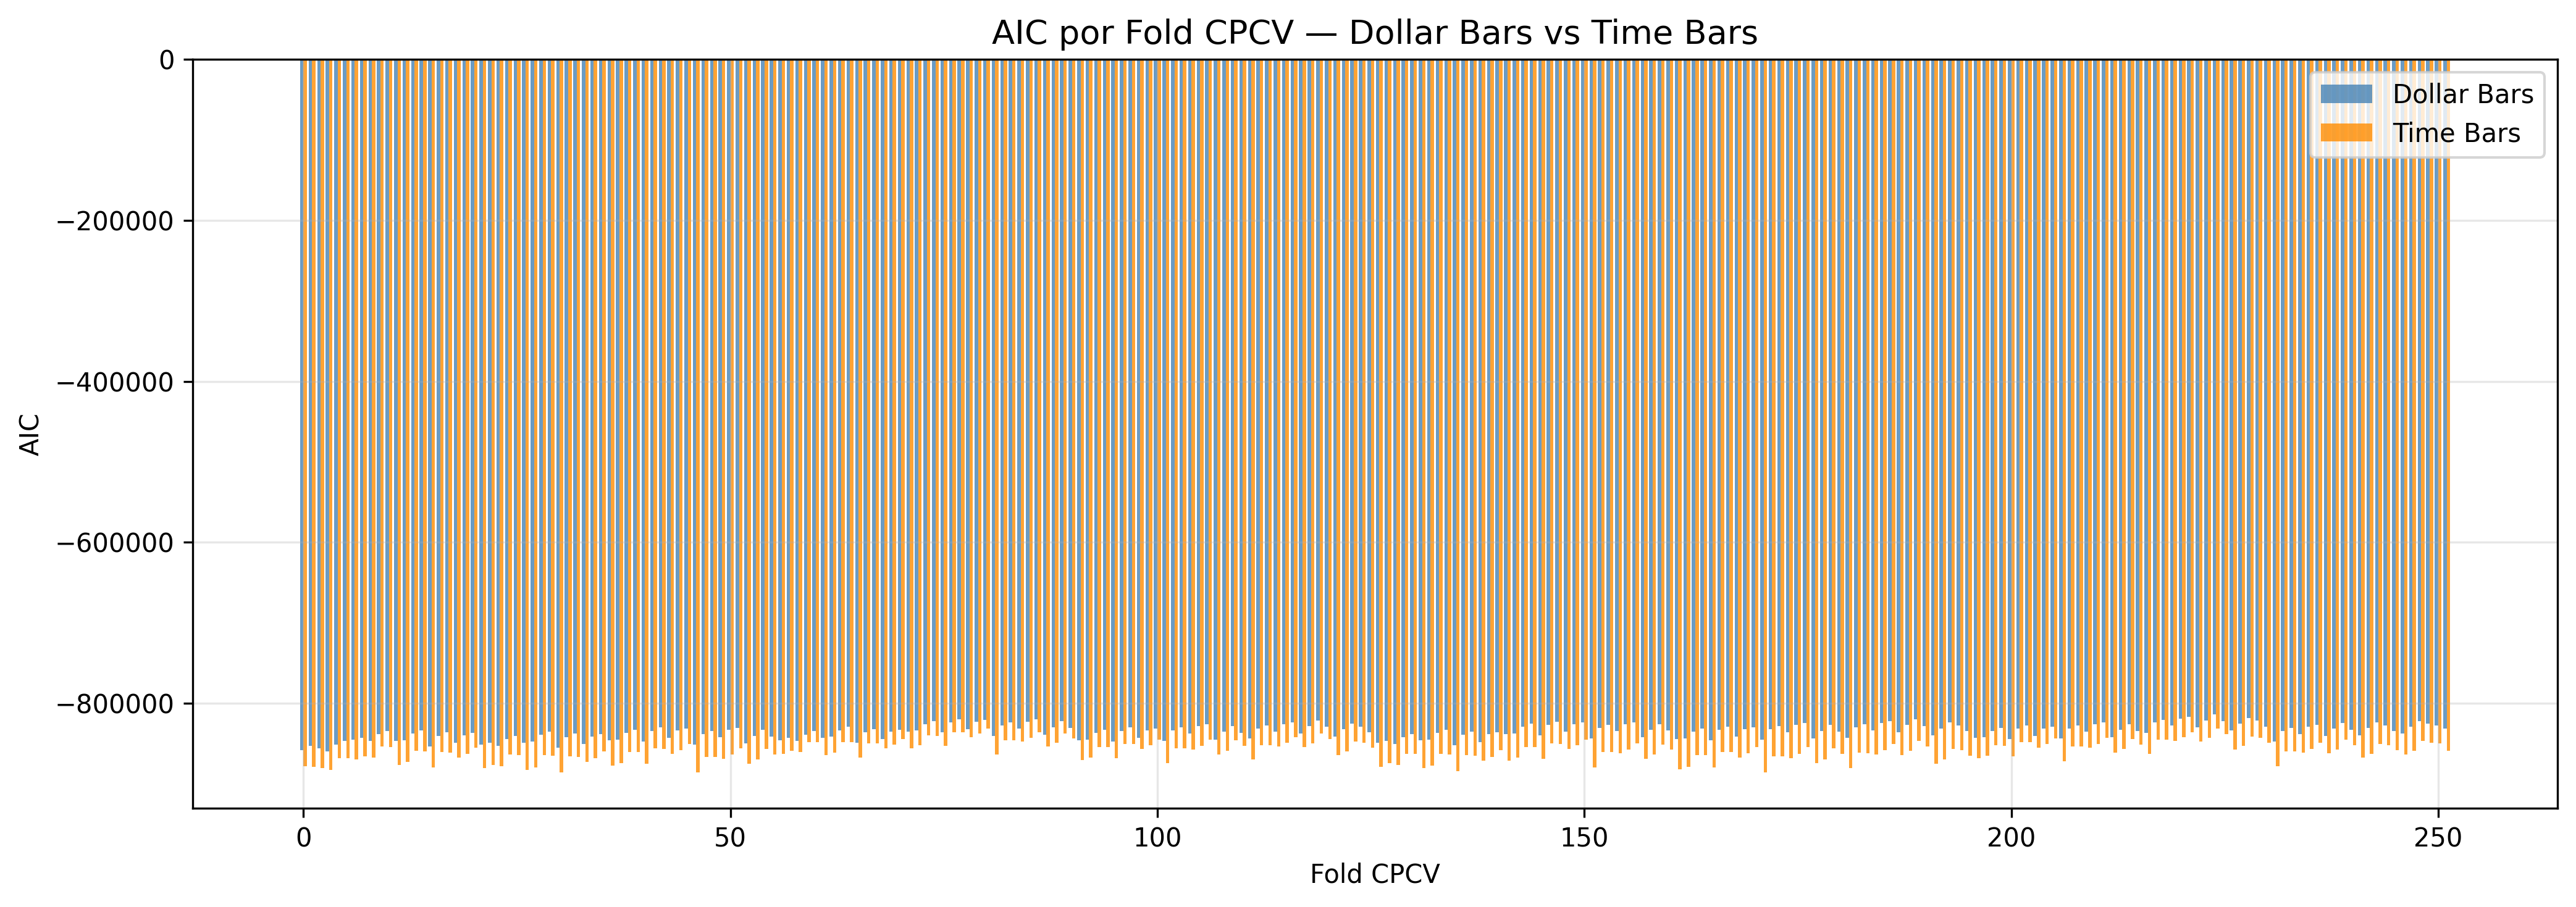
\includegraphics[width=0.95\textwidth]{comparacao_modelos/cpcv_01_aic_por_fold.png}
    \caption{AIC médio por fold CPCV --- Dollar Bars vs.\ Time Bars.}
    \label{fig:cpcv_aic}
\end{figure}

% ==========================================================
\section{Estimação do Modelo Final}
\label{sec:met_estimacao}
% ==========================================================

Após a seleção de parâmetros, o modelo final de cada série foi
reestimado utilizando \textbf{todo} o conjunto de treino (sem
particionamento CPCV), a fim de maximizar a precisão dos coeficientes
estimados. A \autoref{tab:modelo_final} apresenta os critérios de
informação do ajuste final.

\begin{table}[H]
\centering
\caption{Critérios de informação do modelo final estimado sobre o
conjunto de treino completo.}
\label{tab:modelo_final}
\begin{tabular}{llSS}
\toprule
{Série} & {Modelo} & {AIC} & {BIC} \\
\midrule
\emph{Dollar Bars} & GARCH(1,2) & -1693794.21 & -1693744.06 \\
\emph{Time Bars}   & GARCH(1,1) & -1742053.06 & -1742012.92 \\
\bottomrule
\end{tabular}
\fonte{Elaboração própria.}
\end{table}

A partir do modelo estimado, realizou-se a previsão \emph{one-step-ahead}
da variância condicional $\hat{\sigma}_t^2$ para cada observação do
conjunto de teste: 41.926 previsões para \emph{dollar bars} e 42.105 para
\emph{time bars}.

% ==========================================================
\section{Agregação para Nível Diário}
\label{sec:met_agregacao}
% ==========================================================

Como a volatilidade realizada (RV) de referência é calculada em base
diária, as previsões intradiárias de variância condicional precisam ser
agregadas ao nível diário para permitir comparação direta. A agregação
segue o princípio de aditividade da variância de retornos logarítmicos
independentes: a variância diária prevista é obtida pela soma das
variâncias condicionais intradiárias dentro de cada dia:
%
\begin{equation}
    \label{eq:met_agregacao}
    \hat{\sigma}^2_{\text{dia},d} =
    \sum_{t \in \mathcal{B}_d} \hat{\sigma}_t^2,
\end{equation}
%
onde $\mathcal{B}_d$ denota o conjunto de barras pertencentes ao dia $d$.

Após a agregação e o alinhamento com o \emph{benchmark} de volatilidade
realizada, obtiveram-se:

\begin{itemize}
    \item \textbf{Dollar Bars}: 171 dias com previsão (14/jul/2025 a
          31/dez/2025), todos alinhados com o RV \emph{benchmark};
    \item \textbf{Time Bars}: 147 dias com previsão (07/ago/2025 a
          31/dez/2025), todos alinhados com o RV \emph{benchmark}.
\end{itemize}

A diferença na quantidade de dias (171 vs.\ 147) decorre das datas
distintas de início do conjunto de teste para cada tipo de barra,
conforme discutido na \autoref{sec:met_split}. Para garantir comparabilidade
estrita entre os modelos, a avaliação final das métricas, os intervalos
de confiança e o teste de Diebold-Mariano foram calculados exclusivamente
sobre a \textbf{interseção} dos dois períodos: os \textbf{147 dias comuns}
compreendidos entre 07/ago/2025 e 31/dez/2025.

% ==========================================================
\section{Métricas de Avaliação e Testes Estatísticos}
\label{sec:met_metricas}
% ==========================================================

As previsões diárias de variância foram avaliadas contra o \emph{benchmark}
de volatilidade realizada (RV consenso, \autoref{subsec:tsrv}) utilizando
as métricas e testes descritos na \autoref{sec:metricas}. Esta seção
detalha a parametrização específica empregada.

% ----------------------------------------------------------
\subsection{Funções de Perda e Regressão Mincer-Zarnowitz}
\label{subsec:met_funcoes_perda}
% ----------------------------------------------------------

Foram calculadas três funções de perda --- MSE (\autoref{eq:mse}), MAE
(\autoref{eq:mae}) e QLIKE (\autoref{eq:qlike}) --- sobre os pares
$(\hat{\sigma}^2_{\text{dia},d},\, \xi_d)$ para cada tipo de barra, onde
$\xi_d$ denota a volatilidade realizada diária do \emph{benchmark}.

A regressão de Mincer-Zarnowitz (\autoref{eq:mz}) foi estimada por MQO,
fornecendo o coeficiente de determinação $R^2$, o intercepto $\alpha$ e a
inclinação $\beta$, com seus respectivos $p$-valores.

A \autoref{tab:metricas} apresenta os resultados comparativos.

\begin{table}[H]
\centering
\caption{Métricas de avaliação das previsões de variância vs.\ RV
\emph{benchmark}.}
\label{tab:metricas}
\begin{tabular}{lSS}
\toprule
{Métrica} & {\emph{Dollar Bars}} & {\emph{Time Bars}} \\
\midrule
MSE               & 1.05e-7  & 1.65e-7  \\
MAE               & 2.64e-4  & 3.59e-4  \\
QLIKE             & -6.993   & -6.776   \\
$R^2_{\text{MZ}}$ & 0.667    & 0.493    \\
$\hat{\alpha}$    & -9.20e-5 & -2.54e-4 \\
$\hat{\beta}$     & 0.868    & 1.032    \\
\bottomrule
\end{tabular}
\fonte{Elaboração própria.}
\end{table}

% ----------------------------------------------------------
\subsection{Teste de Diebold-Mariano}
\label{subsec:met_dm}
% ----------------------------------------------------------

Para comparar formalmente o poder preditivo dos dois modelos, aplicou-se o
teste de Diebold-Mariano (\autoref{subsec:diebold_mariano}) com a função
de perda MSE. A hipótese nula é de igual poder preditivo entre o modelo
ajustado sobre \emph{dollar bars} e o ajustado sobre \emph{time bars}.

O teste foi calculado sobre o subconjunto de dias em que ambos os modelos
possuem previsões, com correção HAC de Newey-West. Os resultados foram:

\begin{itemize}
    \item Estatística DM: $-4{,}806$;
    \item $p$-valor: $< 0{,}001$.
\end{itemize}

Ao nível de significância de 5\%, \textbf{rejeita-se} a hipótese nula de
igual poder preditivo ($p < 0{,}001$). A estatística negativa indica que
o modelo ajustado sobre \emph{dollar bars} produz perdas MSE
significativamente menores do que o ajustado sobre \emph{time bars},
evidenciando superioridade preditiva estatisticamente distinguível.

% ----------------------------------------------------------
\subsection{Intervalos de Confiança Bootstrap}
\label{subsec:met_bootstrap}
% ----------------------------------------------------------

Intervalos de confiança de 95\% para as métricas pontuais foram
construídos pelo método de \emph{bootstrap} percentil não-paramétrico
(\autoref{subsec:bootstrap_ic}) com $B = 2.000$ reamostras. A
\autoref{tab:bootstrap} apresenta os resultados.

\begin{table}[H]
\centering
\caption{Intervalos de confiança bootstrap (95\%) para as métricas de
avaliação.}
\label{tab:bootstrap}
\begin{tabular}{llScc}
\toprule
{Série} & {Métrica} & {Pontual} & {IC 95\%} & {SE} \\
\midrule
\multirow{3}{*}{\emph{Dollar Bars}}
    & MSE   & 1.050e-7 & {$[7{,}34\text{e-}8;\; 1{,}49\text{e-}7]$} & 1.93e-8 \\
    & MAE   & 2.637e-4 & {$[2{,}35\text{e-}4;\; 2{,}97\text{e-}4]$} & 1.59e-5 \\
    & QLIKE & -6.993   & {$[-7{,}137;\; -6{,}845]$}                  & 7.48e-2 \\
\addlinespace
\multirow{3}{*}{\emph{Time Bars}}
    & MSE   & 1.645e-7 & {$[1{,}35\text{e-}7;\; 2{,}00\text{e-}7]$} & 1.66e-8 \\
    & MAE   & 3.588e-4 & {$[3{,}29\text{e-}4;\; 3{,}90\text{e-}4]$} & 1.56e-5 \\
    & QLIKE & -6.776   & {$[-6{,}877;\; -6{,}668]$}                  & 5.38e-2 \\
\bottomrule
\end{tabular}
\nota{Valores calculados sobre os 147 dias comuns (07/ago/2025--31/dez/2025).
$B = 2.000$ reamostras; IC pelo método percentil.}
\fonte{Elaboração própria.}
\end{table}

Os intervalos de confiança para o MSE \textbf{não se sobrepõem}
($[7{,}34\text{e-}8;\; 1{,}49\text{e-}7]$ vs.\
$[1{,}35\text{e-}7;\; 2{,}00\text{e-}7]$), corroborando a rejeição da
hipótese nula pelo teste de Diebold-Mariano. Para a QLIKE, a ausência de
sobreposição também é verificada, reforçando a superioridade das
\emph{dollar bars} sob essa função de perda robusta \cite{patton2011}.


% =============================================================================
%  CAPÍTULO 4 — RESULTADOS E DISCUSSÃO
%  TCC: Dollar Bars vs. Time Bars — Modelos GARCH para BTC/USDT
% =============================================================================

\chapter{Resultados e Discussão}
\label{cap:resultados}

% -----------------------------------------------------------------------------
\section{Propriedades Estatísticas Comparativas das Séries}
\label{sec:prop_estatisticas}

A análise exploratória das séries de retornos logarítmicos revela diferenças estruturais
substanciais entre as duas formas de amostragem, conforme sintetizado na \autoref{tab:descritivas}.
Essas diferenças não são ruído amostral: elas decorrem diretamente do mecanismo pelo qual
cada tipo de barra é construída.

\begin{table}[H]
\centering
\caption{Estatísticas descritivas dos retornos logarítmicos.}
\label{tab:descritivas}
\begin{tabular}{lSS}
\toprule
{Estatística} & {\emph{Dollar Bars}} & {\emph{Time Bars}} \\
\midrule
Média ($1^{\circ}$ momento)        &  3.46e-6  &  3.44e-6  \\
Variância ($2^{\circ}$ momento)    &  2.49e-6  &  2.40e-6  \\
Assimetria ($3^{\circ}$ momento)   &  0.0547   & -1.0071   \\
Curtose de Fisher ($4^{\circ}$ momento) &  3.0879   &  75.3687  \\
\bottomrule
\end{tabular}
\fonte{Elaboração própria.}
\end{table}

O indicador mais expressivo é a curtose. As time bars de 5 minutos apresentam curtose de Fisher
de 75,37, ao passo que as dollar bars registram apenas 3,09 — uma razão de aproximadamente
25 vezes. Para compreender essa disparidade, é preciso considerar o que ocorre durante
choques de volatilidade no mercado de Bitcoin. Ao longo de um episódio de alta atividade
financeira, dezenas de transações são comprimidas em uma única barra temporal, produzindo
retornos extremamente grandes que inflariam artificialmente as caudas da distribuição.
A dollar bar, ao encerrar uma barra sempre que o volume financeiro transacionado atinge o
limiar $\bar{D}$, redistribui esse mesmo choque ao longo de múltiplas barras, diluindo o
extremo. Esse mecanismo é precisamente a sub-amostragem em períodos de alta atividade
descrita por \citeonline{lopez2018advances} na discussão sobre barras de informação (seção 2.1.1).

A assimetria reforça o mesmo argumento. Enquanto as dollar bars exibem assimetria de apenas
0,05 — praticamente simétrica —, as time bars apresentam assimetria de $-1{,}01$. O sinal
negativo indica que quedas abruptas são capturadas de forma concentrada nessa amostragem:
grandes retornos negativos, correspondentes a correções rápidas, tendem a ocorrer em janelas
de poucos minutos e, por isso, se concentram em uma única barra temporal. Além da implicação
distribucional, a simetria das dollar bars facilita a especificação do modelo GARCH, que,
em sua formulação padrão com inovações gaussianas, assume distribuição condicional simétrica.

\begin{table}[H]
\centering
\caption{Testes de normalidade, estacionariedade e
heteroscedasticidade sobre os retornos logarítmicos.}
\label{tab:testes}
\begin{tabular}{lSSSS}
\toprule
{Teste} &
\multicolumn{2}{c}{\emph{Dollar Bars}} &
\multicolumn{2}{c}{\emph{Time Bars}} \\
\cmidrule(lr){2-3} \cmidrule(lr){4-5}
& {Estat.} & {\emph{p}-valor} & {Estat.} & {\emph{p}-valor} \\
\midrule
Jarque-Bera          & 83384.65  & {$<0{,}001$} & 49860565.37 & {$<0{,}001$} \\
Kolmogorov-Smirnov   & 0.0123    & {$<0{,}001$} & 0.0934      & {$<0{,}001$} \\
\addlinespace
ADF                  & -102.46   & {$<0{,}001$} & -57.32      & {$<0{,}001$} \\
KPSS                 & 0.2053    & 0.10         & 0.2171      & 0.10         \\
\addlinespace
Ljung-Box ($r_t$, lag 10)   & 50.06    & {$<0{,}001$} & 155.03   & {$<0{,}001$} \\
Ljung-Box ($r_t^2$, lag 10) & 79528.20 & {$<0{,}001$} & 28237.22 & {$<0{,}001$} \\
ARCH de Engle (lag 10)      & 30420.71 & {$<0{,}001$} & 24064.78 & {$<0{,}001$} \\
\bottomrule
\end{tabular}
\nota{H$_0$ por teste: Jarque-Bera e KS --- normalidade;
ADF --- raiz unitária; KPSS --- estacionariedade;
Ljung-Box e ARCH de Engle --- ausência de autocorrelação/efeito ARCH.}
\fonte{Elaboração própria.}
\end{table}

\begin{figure}[H]
    \centering
    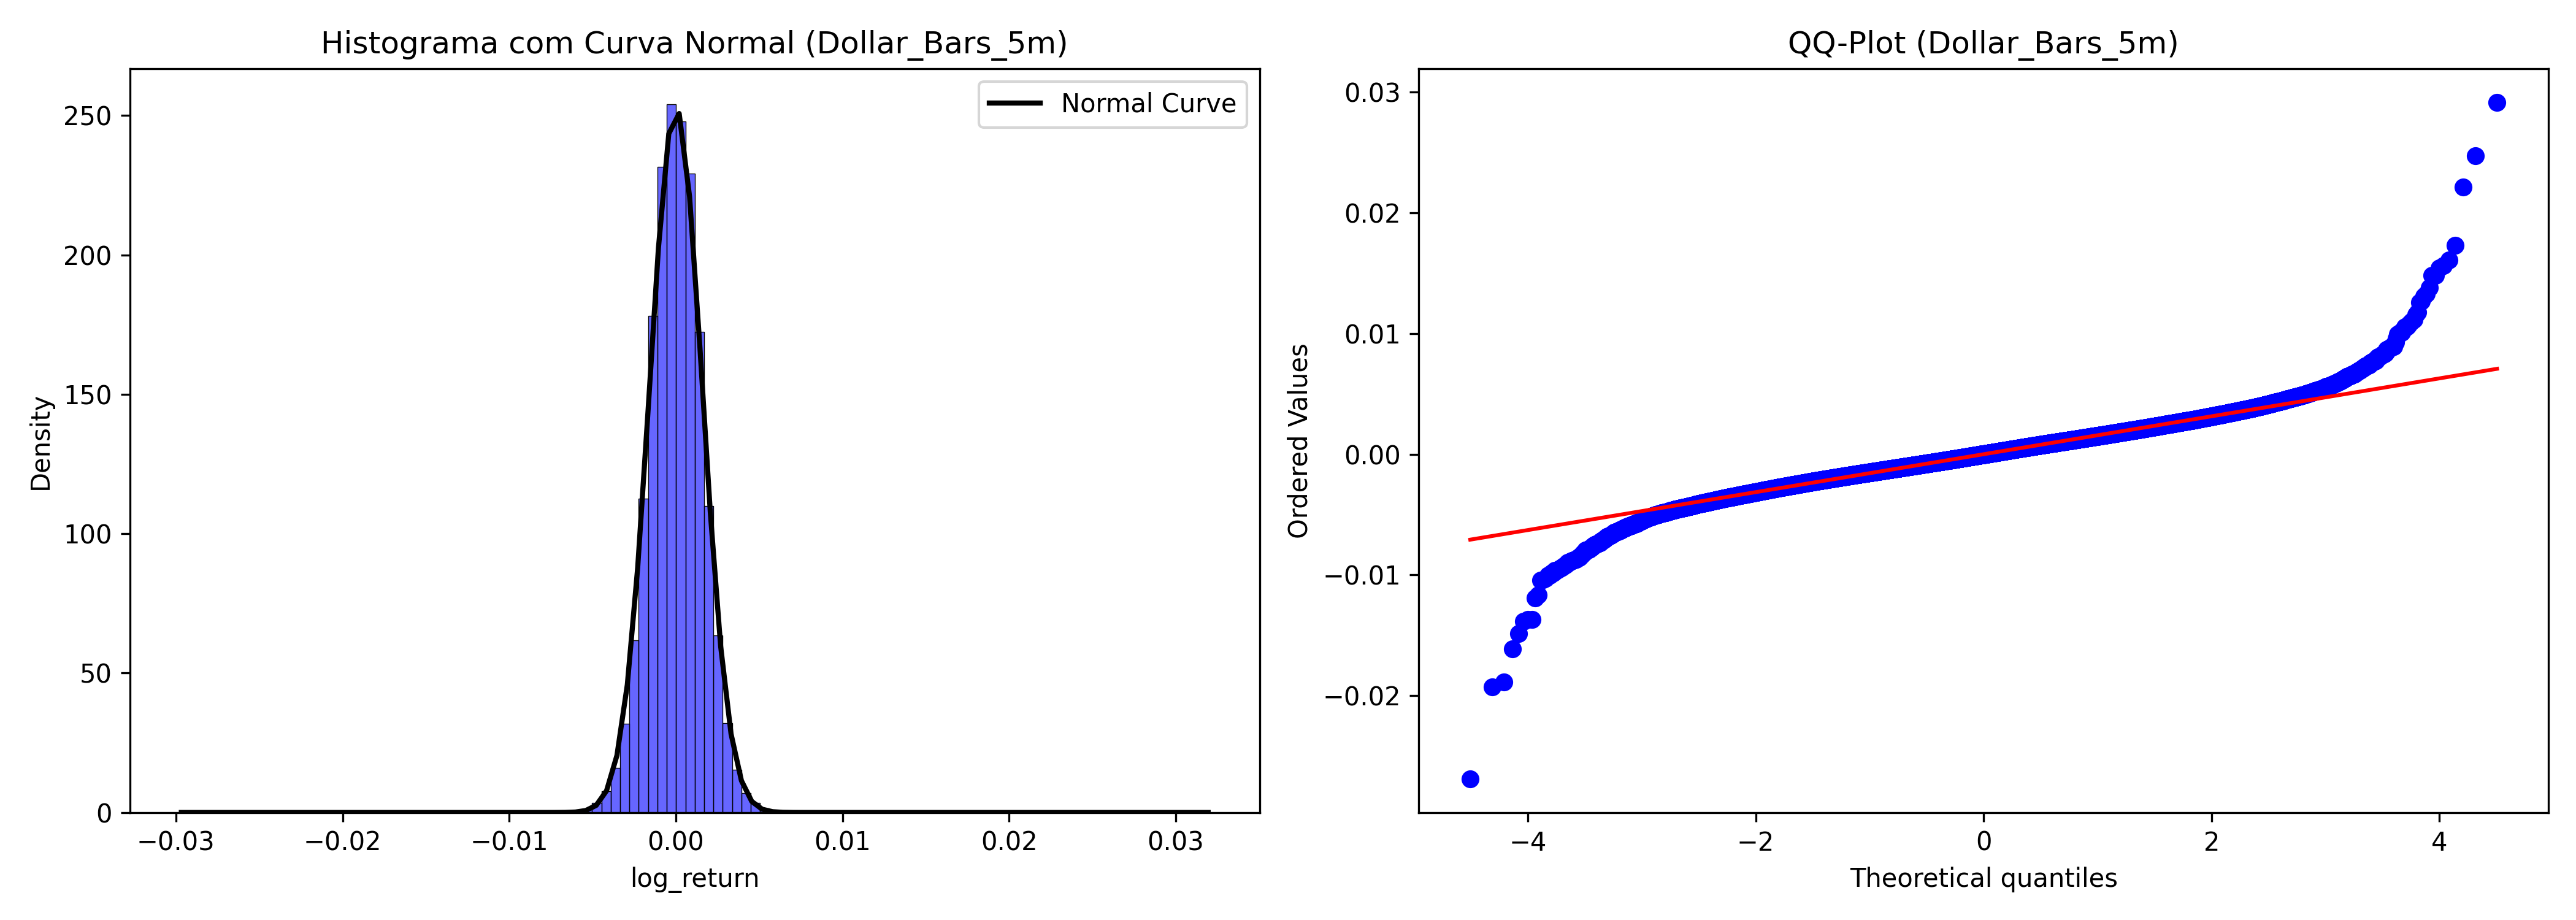
\includegraphics[width=0.95\textwidth]{Dollar_Bars_5m_normalidade.png}
    \caption{Histograma com curva normal e QQ-Plot --- Dollar Bars (5 min).}
    \label{fig:normalidade_dollar}
\end{figure}

\begin{figure}[H]
    \centering
    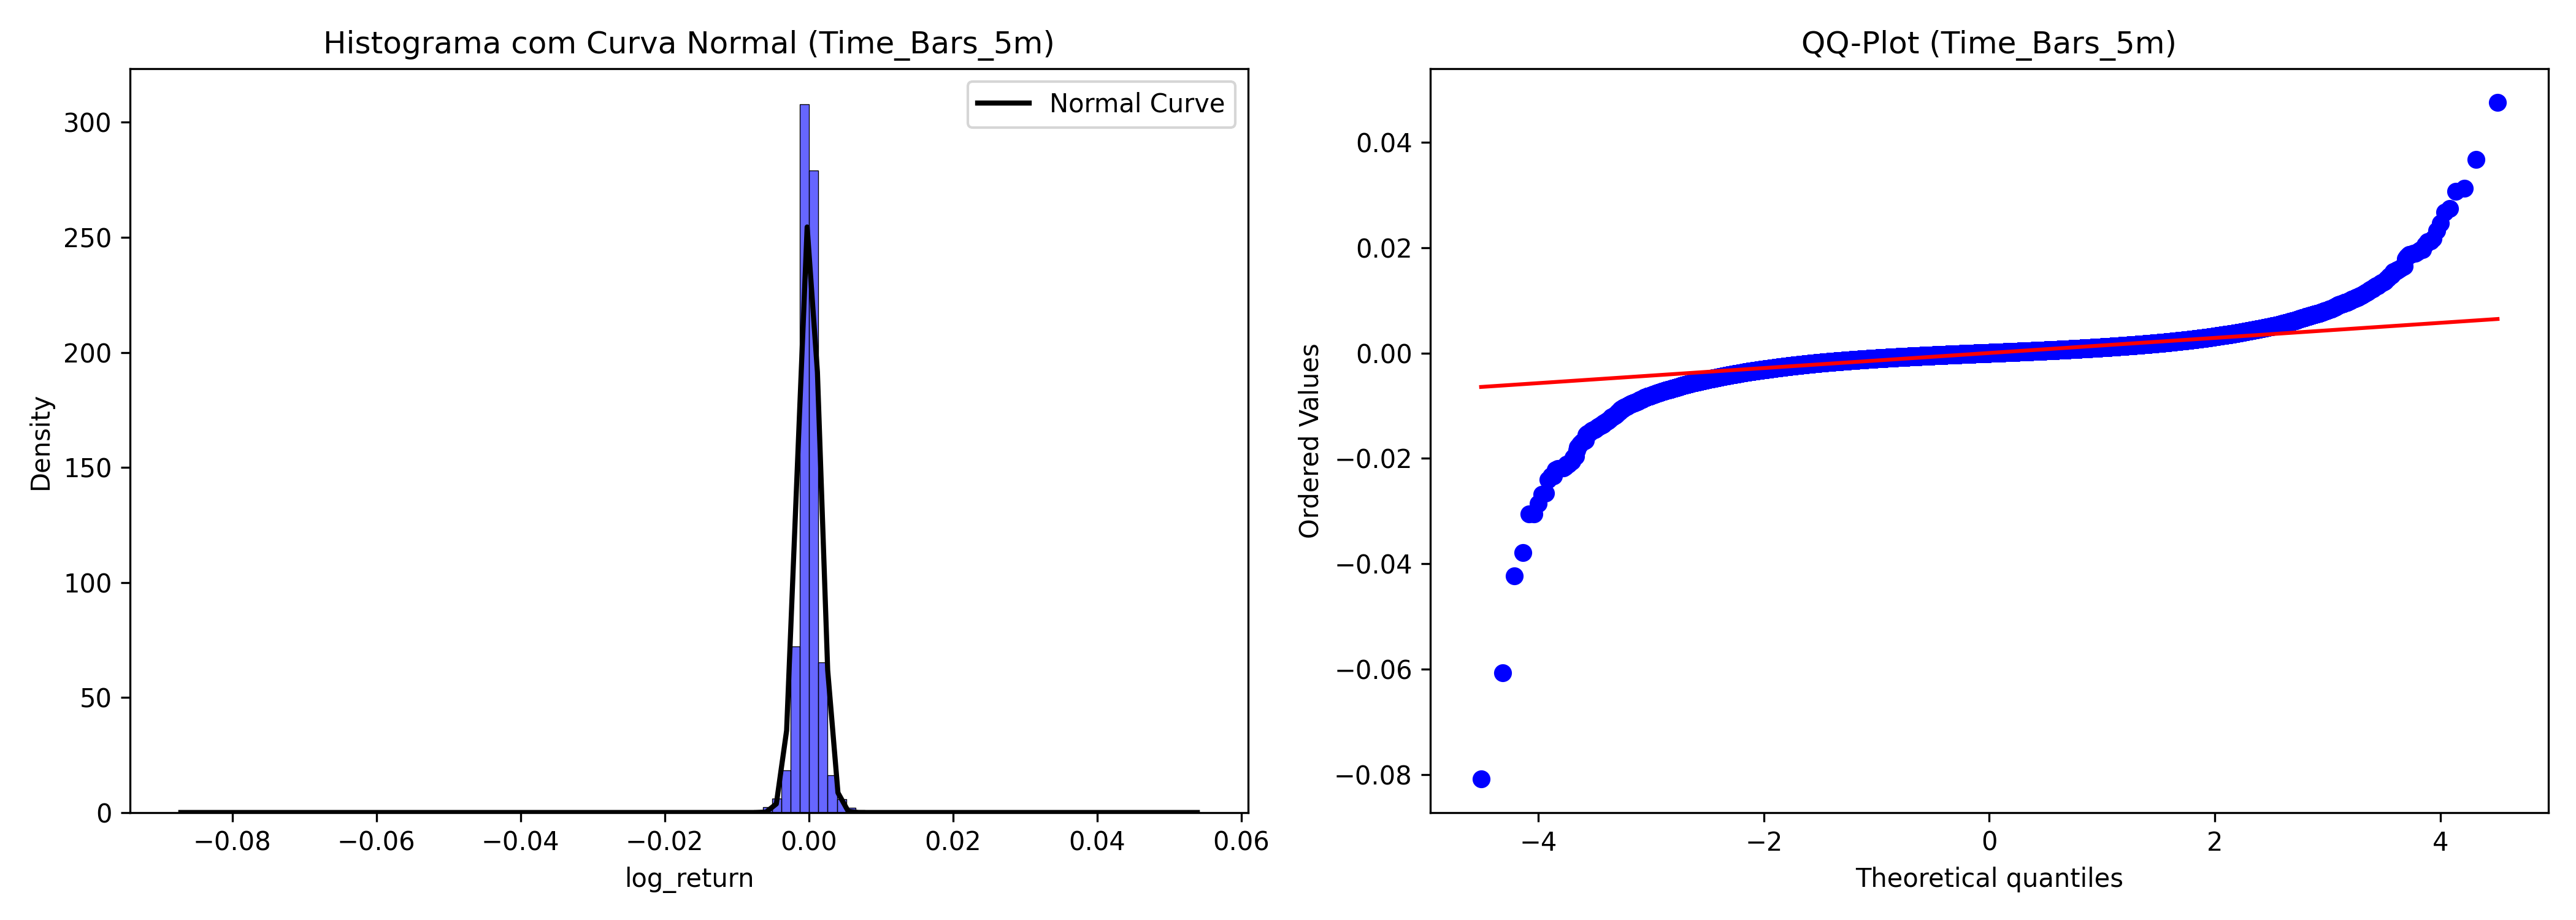
\includegraphics[width=0.95\textwidth]{Time_Bars_5m_normalidade.png}
    \caption{Histograma com curva normal e QQ-Plot --- Time Bars (5 min).}
    \label{fig:normalidade_time}
\end{figure}

\begin{figure}[H]
    \centering
    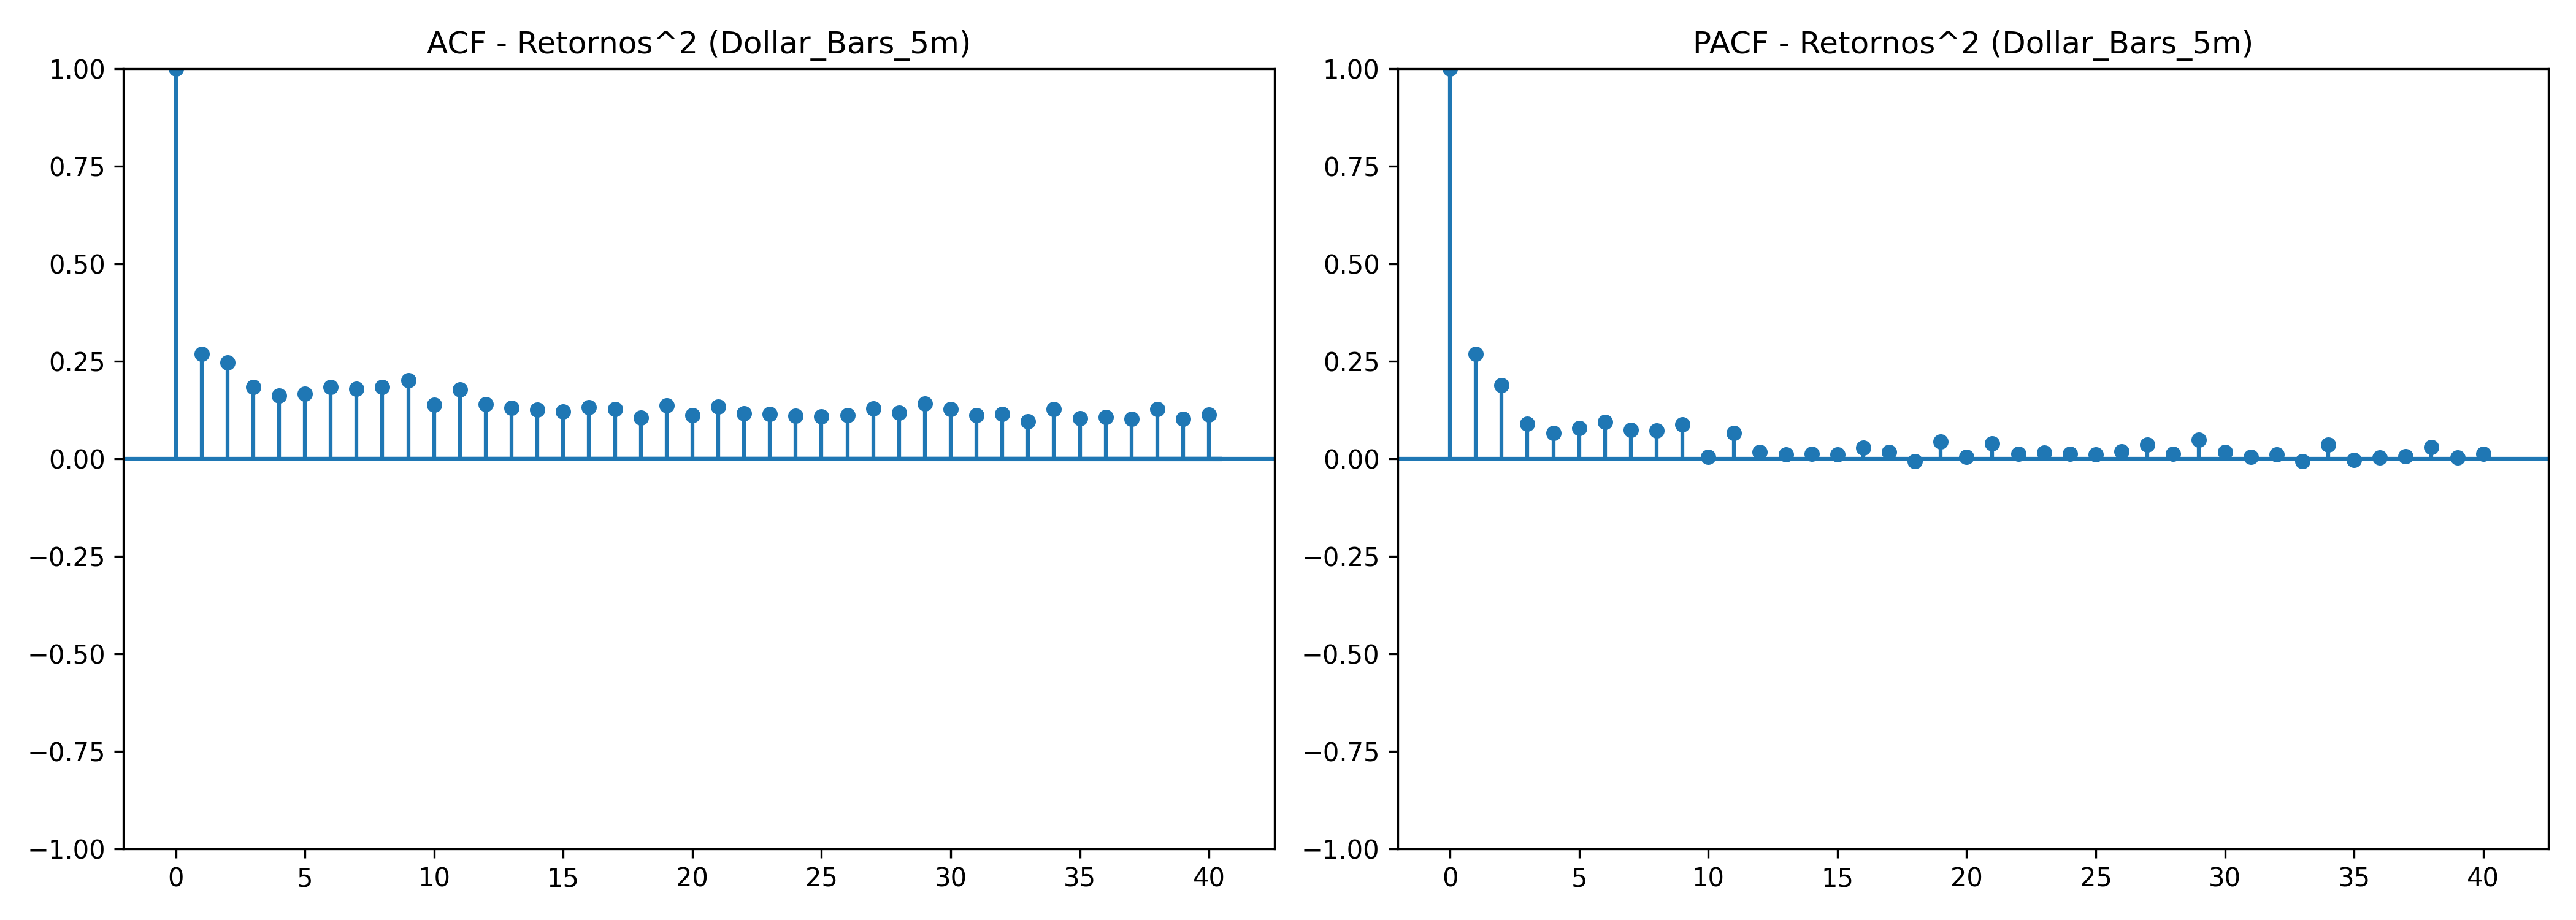
\includegraphics[width=0.95\textwidth]{Dollar_Bars_5m_acf_pacf_retornos2.png}
    \caption{ACF e PACF dos retornos ao quadrado --- Dollar Bars (5 min).}
    \label{fig:acf_dollar_sq}
\end{figure}

\begin{figure}[H]
    \centering
    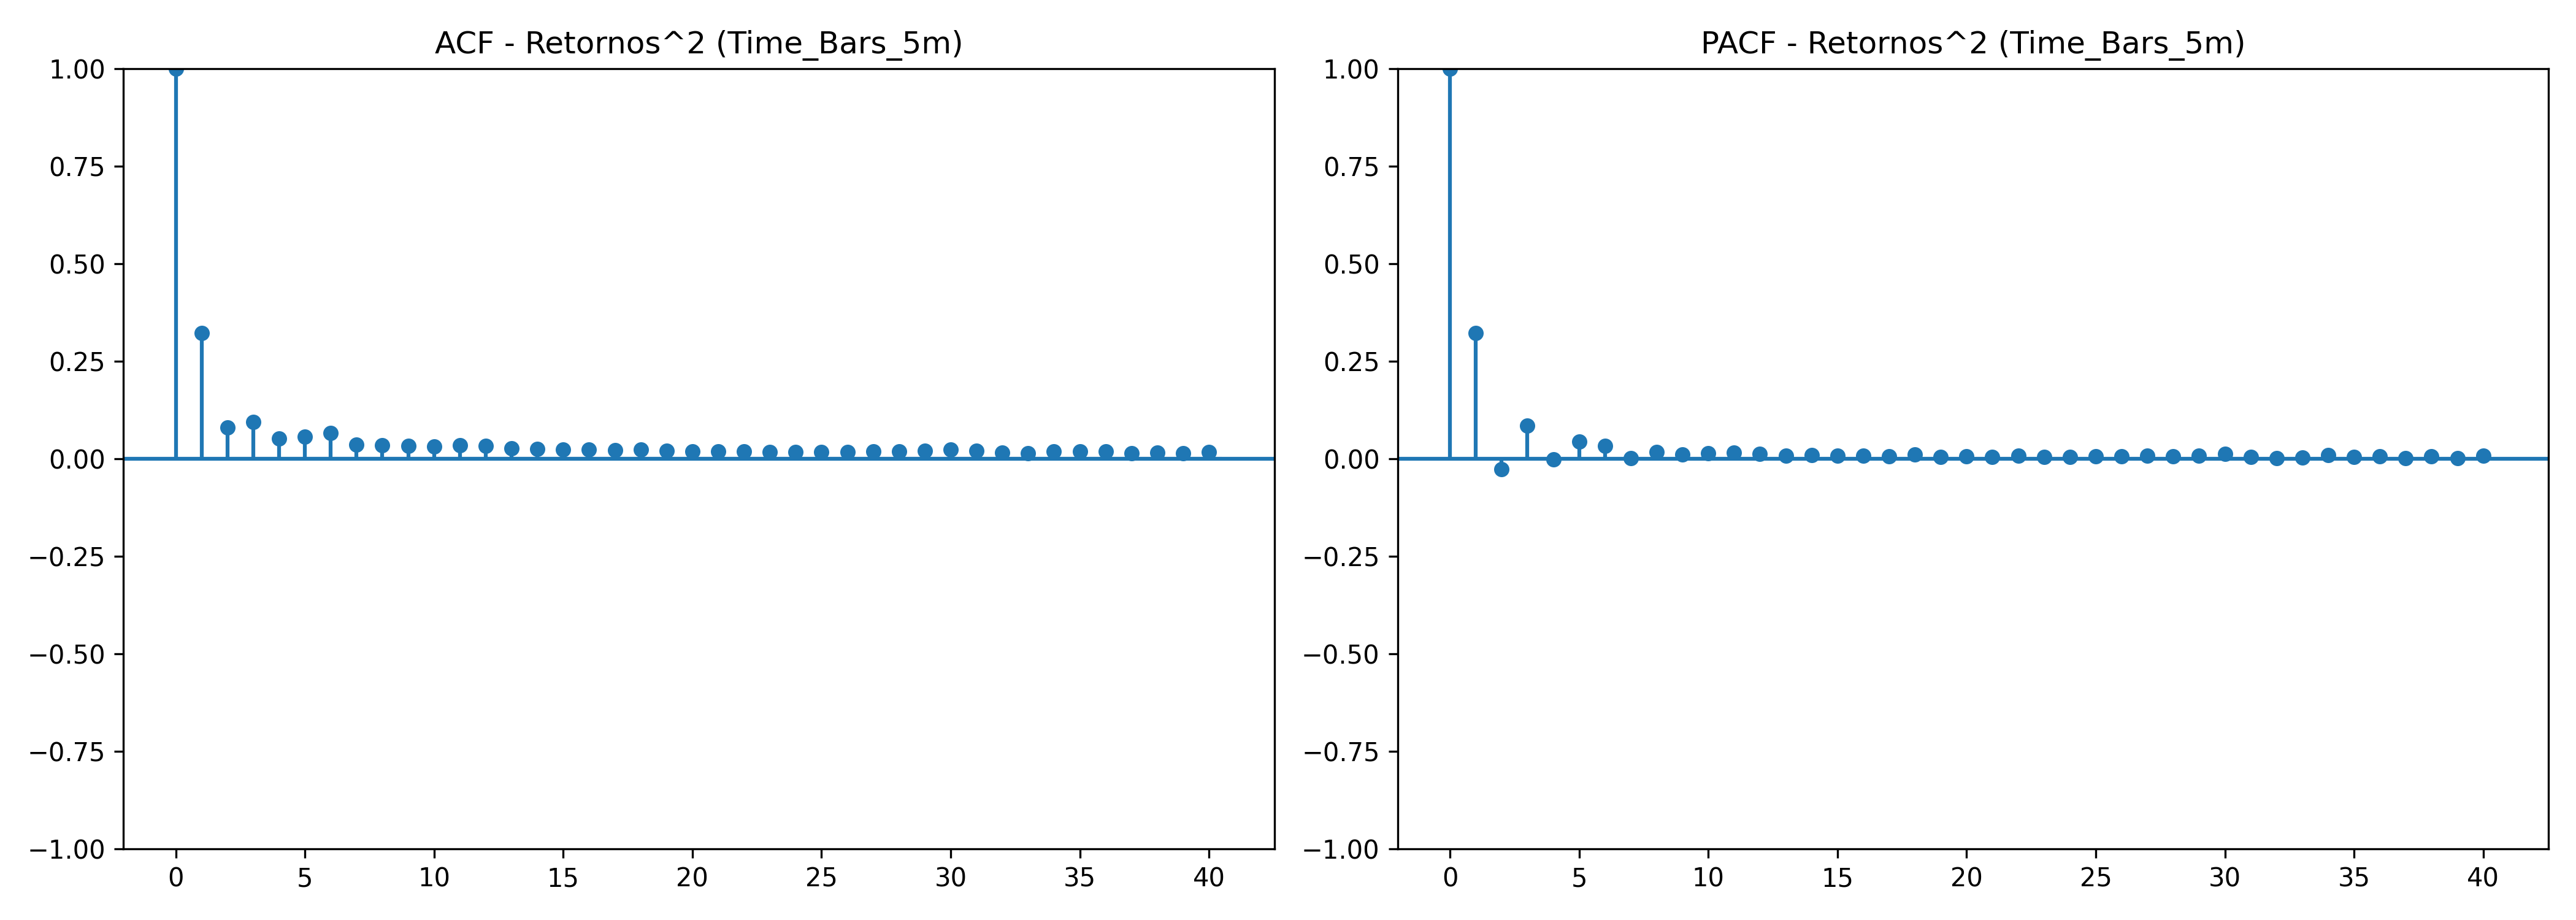
\includegraphics[width=0.95\textwidth]{Time_Bars_5m_acf_pacf_retornos2.png}
    \caption{ACF e PACF dos retornos ao quadrado --- Time Bars (5 min).}
    \label{fig:acf_time_sq}
\end{figure}

Os testes formais de adequação distribucional, apresentados na \autoref{tab:testes},
amplificam esse quadro. A estatística de Jarque-Bera das time bars é superior a 49 milhões,
contra aproximadamente 83 mil para as dollar bars — uma diferença de mais de 500 vezes.
Esse resultado não representa apenas rejeição da normalidade, que ambas as séries exibem:
indica que as caudas das time bars pertencem a uma ordem de magnitude distinta. O teste
de Ljung-Box nos retornos em nível rejeita a hipótese de ausência de autocorrelação
para as duas séries, mas com estatística consideravelmente maior para as time bars
(155,03 versus 50,06). Contudo, conforme discutido na seção seguinte, essa autocorrelação
é de magnitude modesta para o volume de observações disponível e não justifica componentes
autorregressivos ou de médias móveis no modelo final. Ambas as séries são estacionárias:
o teste Dickey-Fuller Aumentado rejeita a hipótese de raiz unitária, e o teste KPSS não
rejeita estacionariedade em nenhuma das duas amostras, validando o uso de $d = 0$ na
especificação ARMA.

Em conjunto, os resultados exploratórios corroboram a hipótese de \citeonline{lopez2018advances}:
dollar bars produzem séries com propriedades distribucionais superiores em termos de
curtose, assimetria e dependência linear residual. Cabe ressalvar, contudo, que propriedades
descritivas melhores não garantem, por si só, maior poder preditivo fora da amostra.
Essa questão é investigada nas seções seguintes.

% -----------------------------------------------------------------------------
\section{Seleção de Modelos via CPCV}
\label{sec:selecao_modelos}

O procedimento de seleção de hiperparâmetros via \textit{Combinatorial Purged Cross-Validation}
(CPCV) com $N = 10$ grupos, $K = 5$ grupos de teste e embargo de 240 barras gerou
$\binom{10}{5} = 252$ folds de avaliação, totalizando 36.288 ajustes MLE por série
(252 folds $\times$ 144 combinações de parâmetros no grid
$\text{ARMA}(0..5,\,0..5) \times \text{GARCH}(1..2,\,1..2)$).

\begin{table}[H]
\centering
\caption{Resultados da seleção de parâmetros via CPCV.}
\label{tab:cpcv_resultados}
\begin{tabular}{llrl}
\toprule
{Série} & {Modelo selecionado} & {Frequência} & {AIC médio} \\
\midrule
\emph{Dollar Bars} & ARMA(0,0)-GARCH(1,2) & 233/252 (92,5\%) &
    $-835.475$ \\
\emph{Time Bars}   & ARMA(0,0)-GARCH(1,1) & 252/252 (100\%) &
    $-859.083$ \\
\bottomrule
\end{tabular}
\fonte{Elaboração própria.}
\end{table}

\begin{figure}[H]
    \centering
    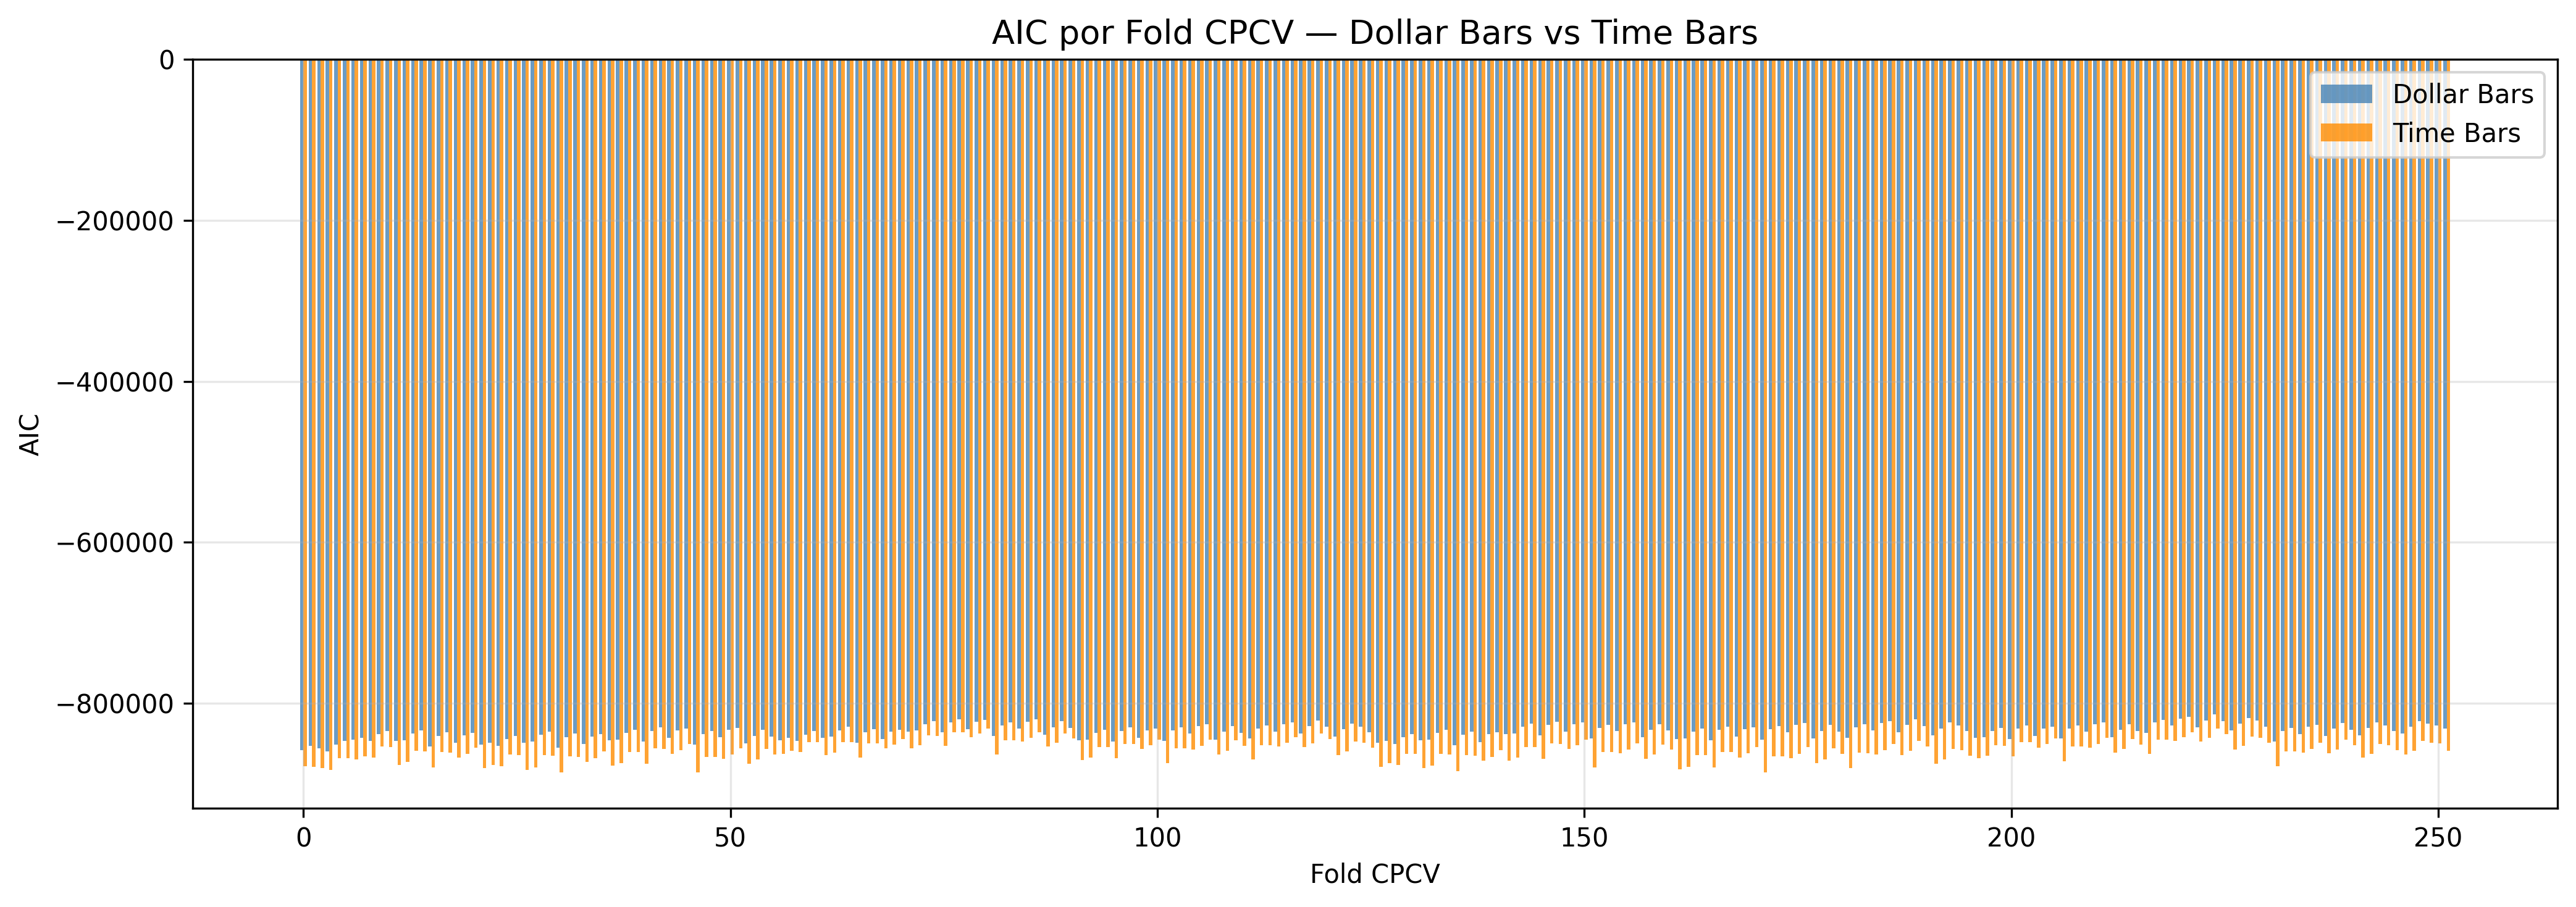
\includegraphics[width=0.95\textwidth]{comparacao_modelos/cpcv_01_aic_por_fold.png}
    \caption{AIC médio por fold CPCV --- Dollar Bars vs.\ Time Bars.}
    \label{fig:cpcv_aic}
\end{figure}

Em ambas as séries, o componente ARMA selecionado foi ARMA$(0,0)$, ou seja, média constante
sem termos autorregressivos nem de médias móveis. Esse resultado é consistente com a
hipótese de eficiência de mercado na forma fraca: os retornos do par BTC/USDT, a despeito
de sua curtose elevada, não apresentam estrutura linear preditível suficiente para justificar
a inclusão de termos AR ou MA. É importante observar que esse resultado não contradiz a
rejeição do Ljung-Box reportada na seção anterior. As autocorrelações detectadas são de
magnitude prática pequena — estatísticas de 50 e 155 para séries com cerca de 200 mil
observações representam efeitos de baixa amplitude — e concentram-se, sobretudo, nos
retornos ao quadrado, não nos níveis; o componente GARCH é o mecanismo mais adequado
para capturá-las.

O resultado mais informativo da seleção refere-se ao componente GARCH. Para as dollar bars,
o modelo GARCH$(1,2)$ --- com um termo de inovação ao quadrado $(\alpha_1)$ e dois termos
de variância defasada $(\beta_1, \beta_2)$ --- foi escolhido em 233 dos 252 folds,
correspondendo a 92,5\% de frequência de seleção. Para as time bars, o modelo GARCH$(1,1)$
canônico foi selecionado na totalidade dos 252 folds (100,0\%). O AIC médio das time bars
ao longo dos folds foi de $-859.083$, contra $-835.475$ para as dollar bars.

A necessidade de um termo $\beta_2$ adicional nas dollar bars tem uma interpretação
econômica plausível. Por construção, as dollar bars possuem espaçamento temporal irregular:
são geradas em maior número durante períodos de alta atividade financeira, quando a
volatilidade do mercado é tipicamente mais elevada. Esse mecanismo faz com que os choques
de volatilidade sejam distribuídos ao longo de mais barras, tornando o decaimento da
variância condicional mais gradual e demandando uma especificação ligeiramente mais rica
para capturá-lo adequadamente. As time bars, ao ignorar esse padrão de irregularidade
temporal, comprimem os choques em barras únicas e produzem uma dinâmica de volatilidade
mais diretamente capturada pelo GARCH$(1,1)$ canônico.

A estabilidade das seleções merece atenção. O fato de o GARCH$(1,1)$ ter sido eleito
em 100\% dos folds para as time bars indica que a dinâmica de volatilidade dessa série
é bem descrita pela especificação padrão da literatura, com pouca ambiguidade quanto à
ordem. Para as dollar bars, a frequência de 92,5\% tampouco é marginal: denota robustez
do GARCH$(1,2)$, não um artefato de um fold específico. Em síntese, o CPCV entregou
seleções estáveis para ambas as séries, com a diferença de especificação entre elas
refletindo uma propriedade genuína das dinâmicas de volatilidade subjacentes.

Cabe destacar que ajuste \textit{in-sample} superior não implica, necessariamente,
melhor desempenho preditivo fora da amostra — distinção fundamental em qualquer
avaliação de modelos de previsão \cite{diebold2015}. Essa questão é endereçada
diretamente na seção seguinte.

A \autoref{tab:modelo_final} apresenta os critérios de informação do
modelo final estimado sobre o conjunto de treino completo.

\begin{table}[H]
\centering
\caption{Critérios de informação do modelo final estimado sobre o
conjunto de treino completo.}
\label{tab:modelo_final}
\begin{tabular}{llSS}
\toprule
{Série} & {Modelo} & {AIC} & {BIC} \\
\midrule
\emph{Dollar Bars} & GARCH(1,2) & -1693794.21 & -1693744.06 \\
\emph{Time Bars}   & GARCH(1,1) & -1742053.06 & -1742012.92 \\
\bottomrule
\end{tabular}
\fonte{Elaboração própria.}
\end{table}

% -----------------------------------------------------------------------------
\section{Desempenho Preditivo Fora da Amostra}
\label{sec:desempenho_previsao}

Esta seção constitui o núcleo analítico do trabalho, respondendo diretamente à pergunta
de pesquisa com base nas métricas calculadas sobre os conjuntos de teste — 171 dias para
as dollar bars (2025-07-14 a 2025-12-31) e 147 dias para as time bars
(2025-08-07 a 2025-12-31) — e comparadas contra o estimador TSRV de volatilidade
realizada como benchmark.

% -----------------------------------------------------------------------------
\subsection{Visualização das Previsões}
\label{subsec:visualizacao_previsao}

Os gráficos a seguir apresentam a série temporal das previsões de variância
condicional agregada ao nível diário em comparação à volatilidade realizada
(TSRV), bem como os erros de previsão ao longo do período de teste.

\begin{figure}[H]
    \centering
    \begin{minipage}[t]{0.48\textwidth}
        \centering
        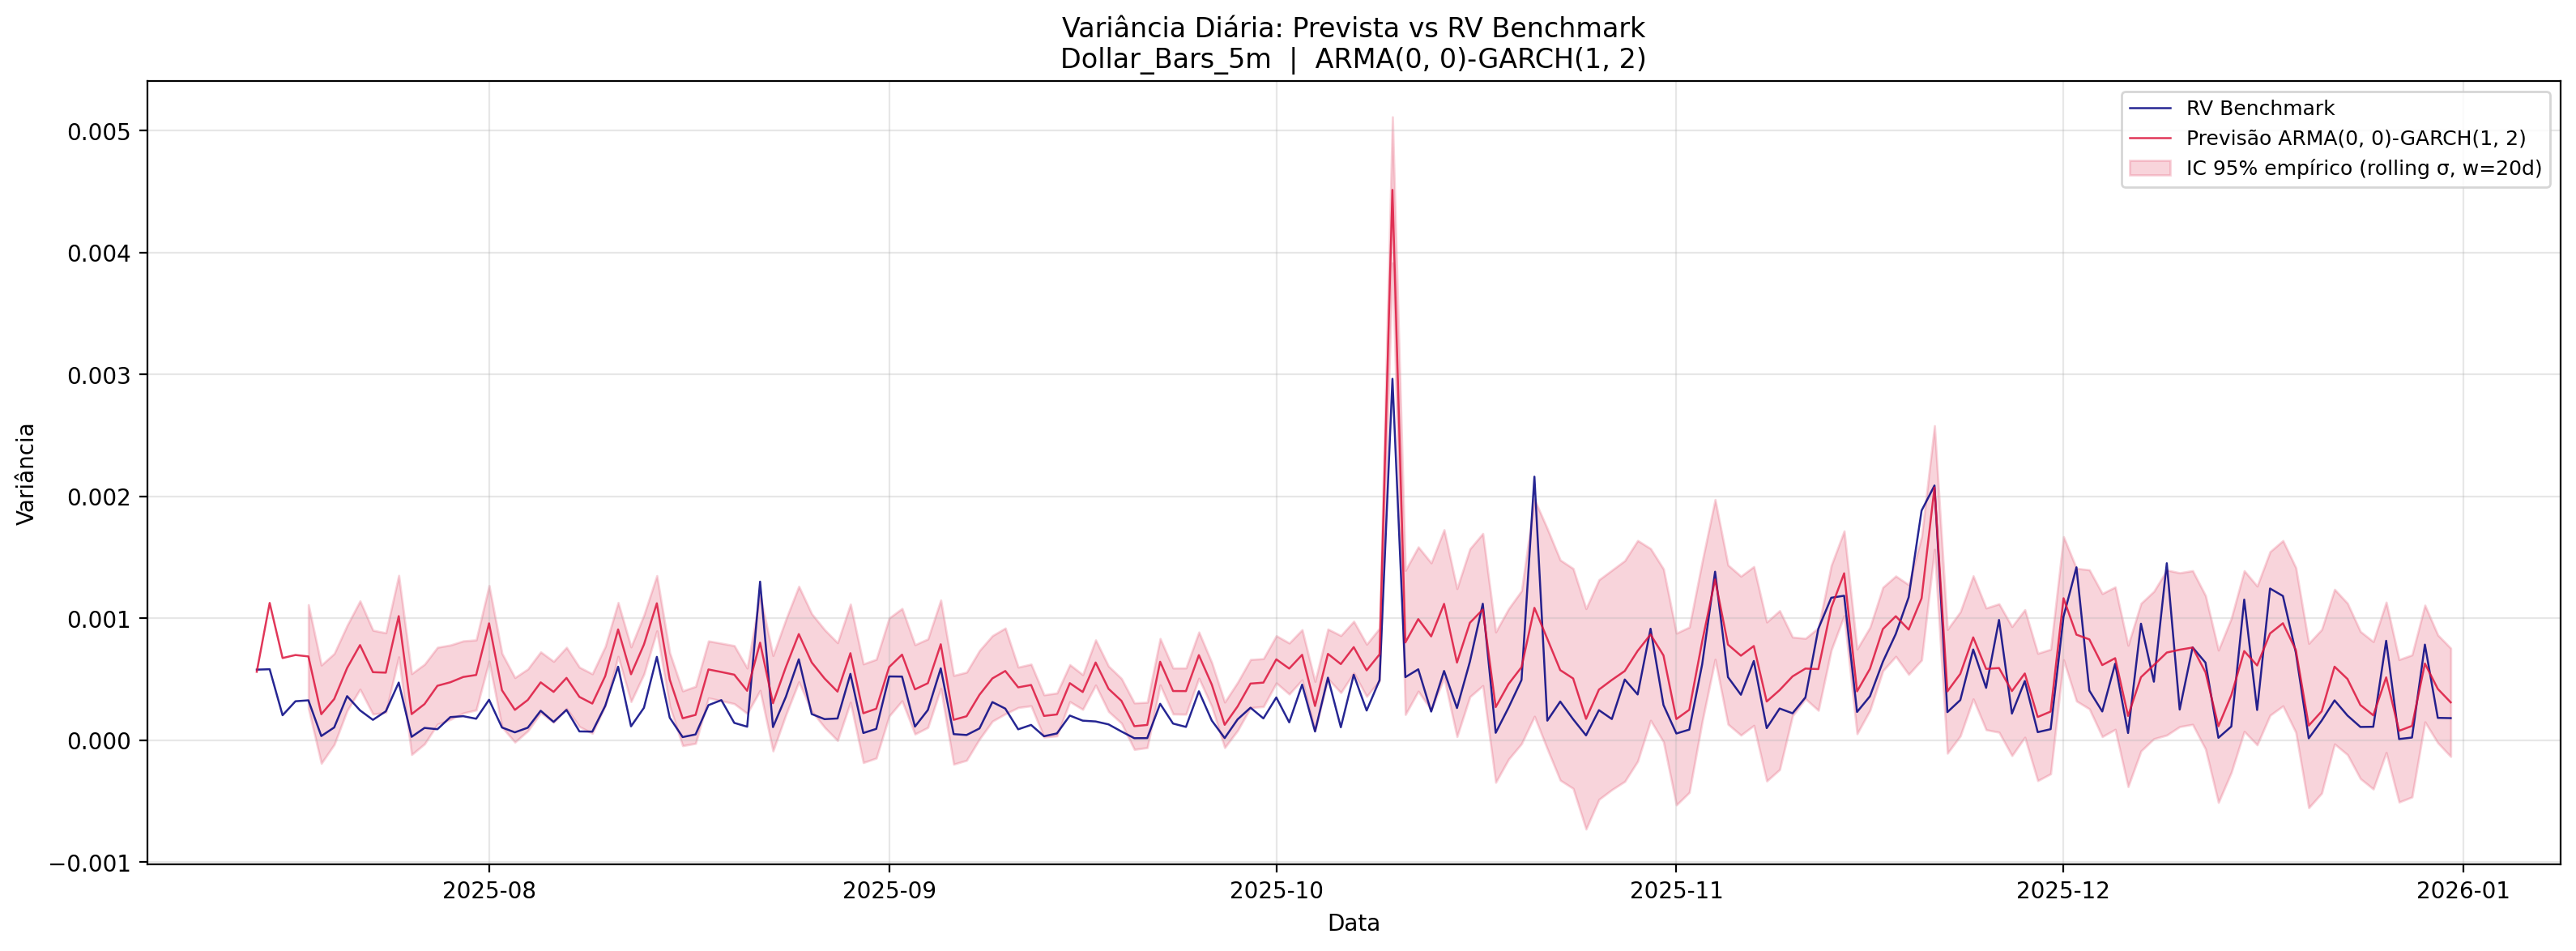
\includegraphics[width=\textwidth]{analise_previsao/Dollar_Bars_5m/Dollar_Bars_5m_01_serie_temporal_ic.png}
        \subcaption{Série temporal com IC \textit{bootstrap} (95\%).}
        \label{fig:prev_dollar_serie}
    \end{minipage}
    \hfill
    \begin{minipage}[t]{0.48\textwidth}
        \centering
        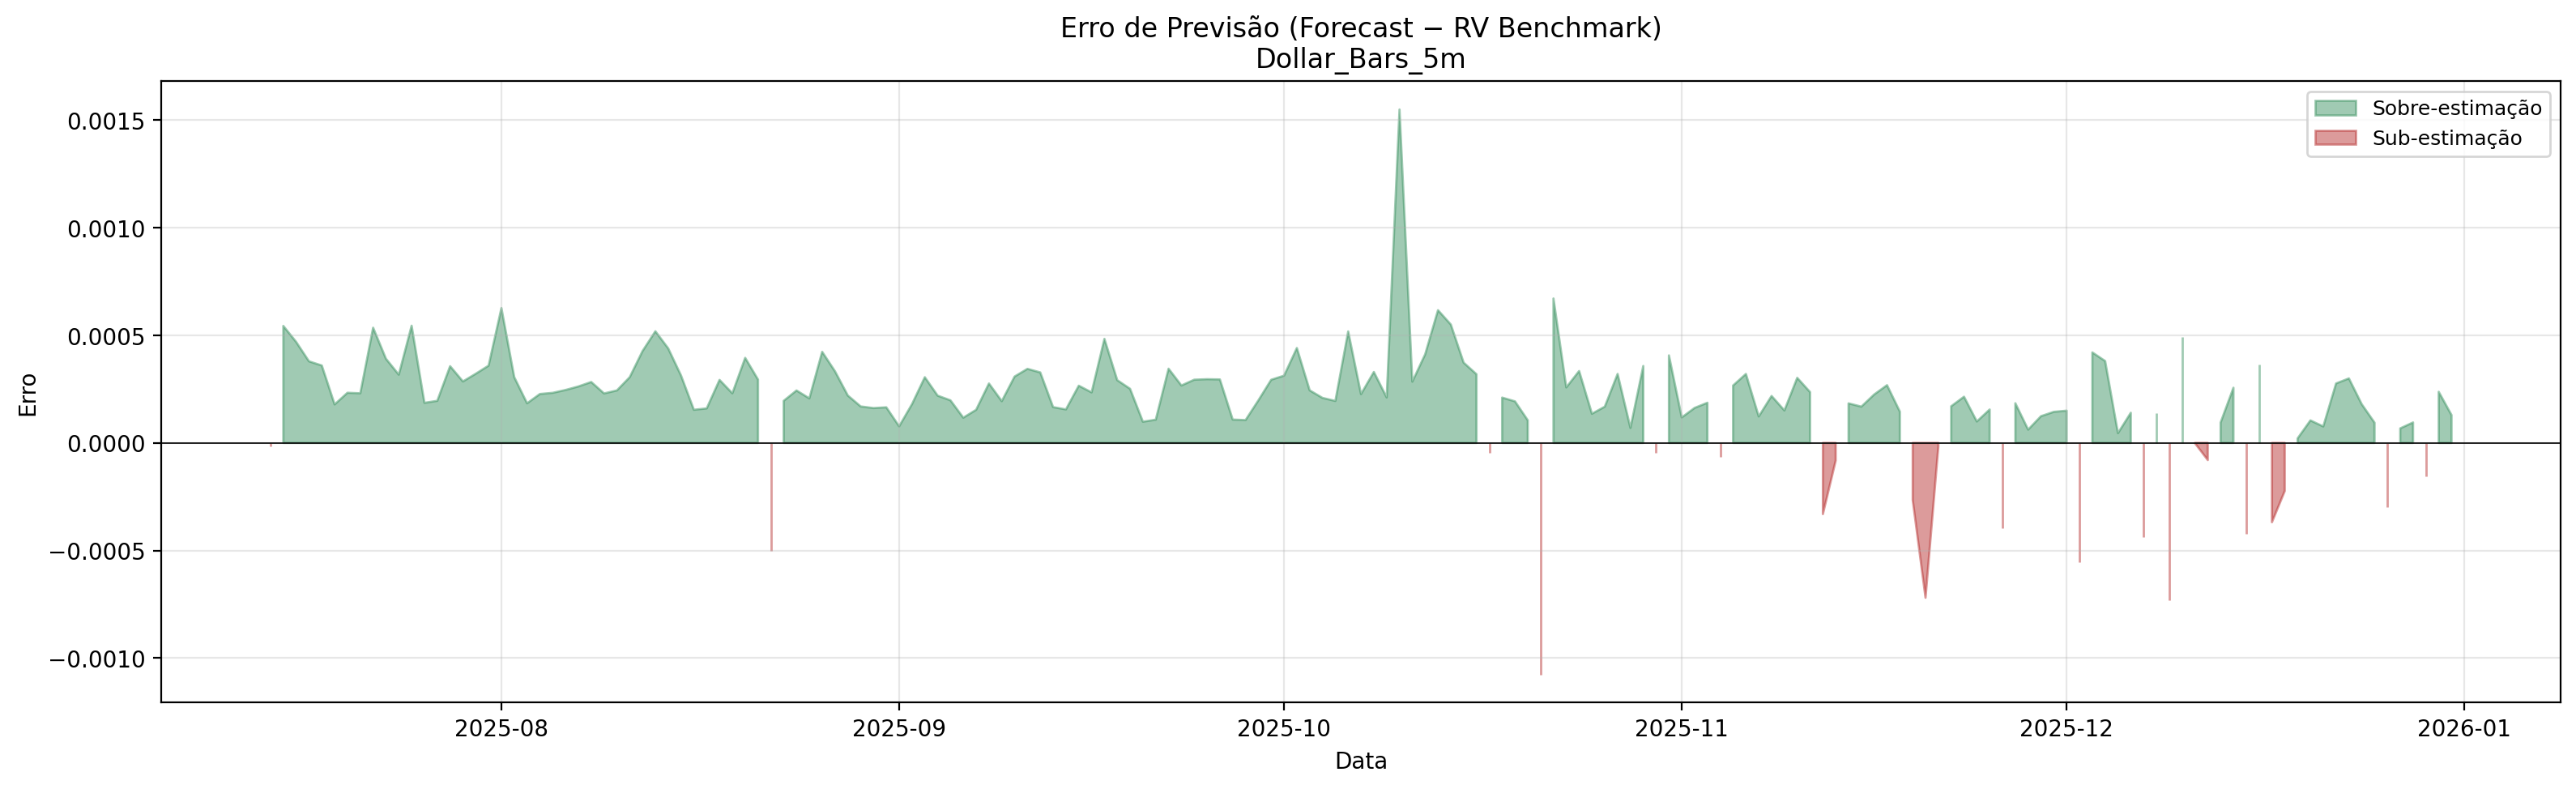
\includegraphics[width=\textwidth]{analise_previsao/Dollar_Bars_5m/Dollar_Bars_5m_02_erro_previsao.png}
        \subcaption{Erros de previsão.}
        \label{fig:prev_dollar_erro}
    \end{minipage}
    \caption{Previsão da variância condicional versus variância realizada (TSRV) --- \emph{Dollar Bars} GARCH(1,2), período de teste (14/jul/2025--31/dez/2025).}
    \label{fig:prev_dollar_grid}
\end{figure}

\begin{figure}[H]
    \centering
    \begin{minipage}[t]{0.48\textwidth}
        \centering
        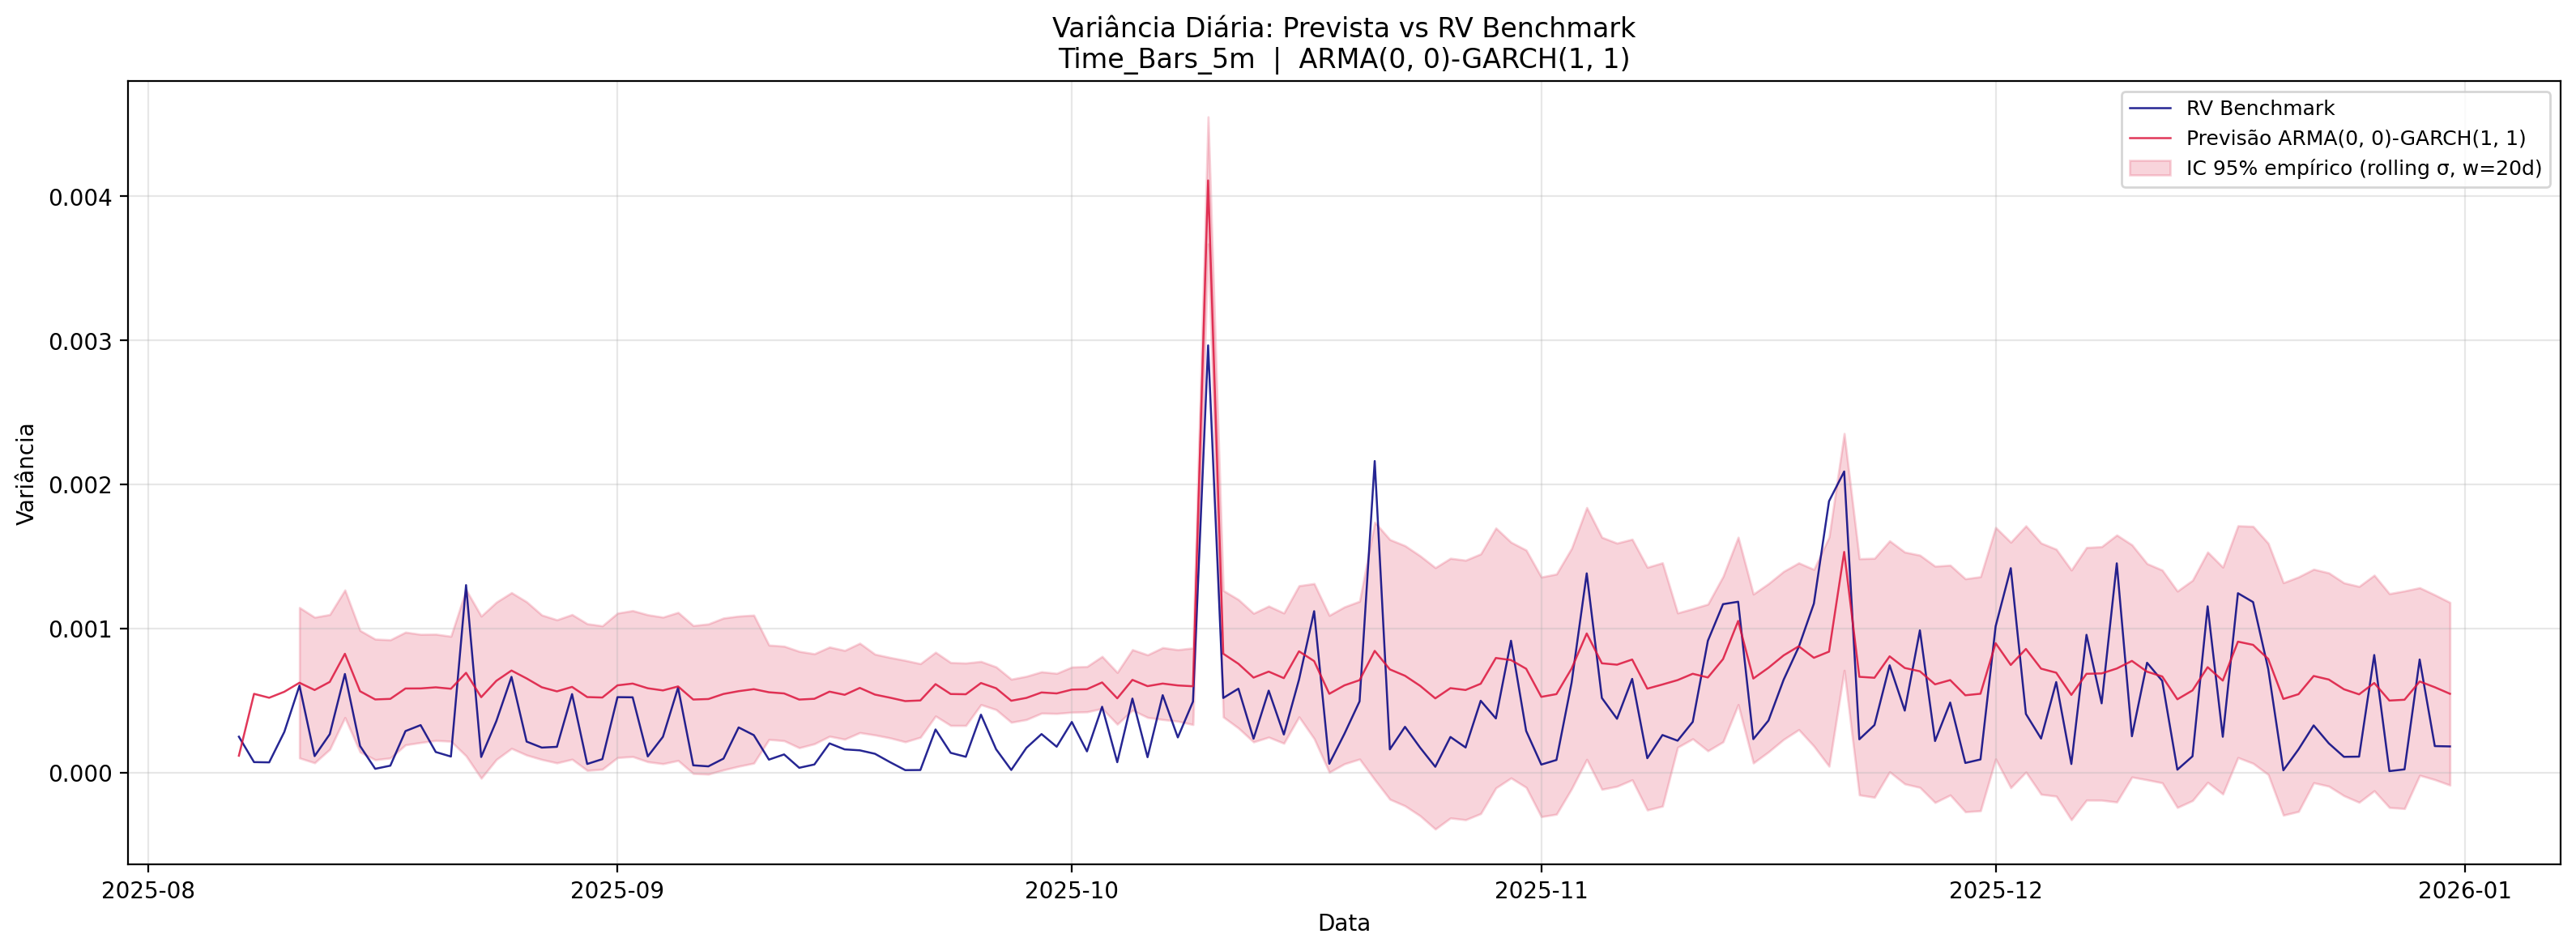
\includegraphics[width=\textwidth]{analise_previsao/Time_Bars_5m/Time_Bars_5m_01_serie_temporal_ic.png}
        \subcaption{Série temporal com IC \textit{bootstrap} (95\%).}
        \label{fig:prev_time_serie}
    \end{minipage}
    \hfill
    \begin{minipage}[t]{0.48\textwidth}
        \centering
        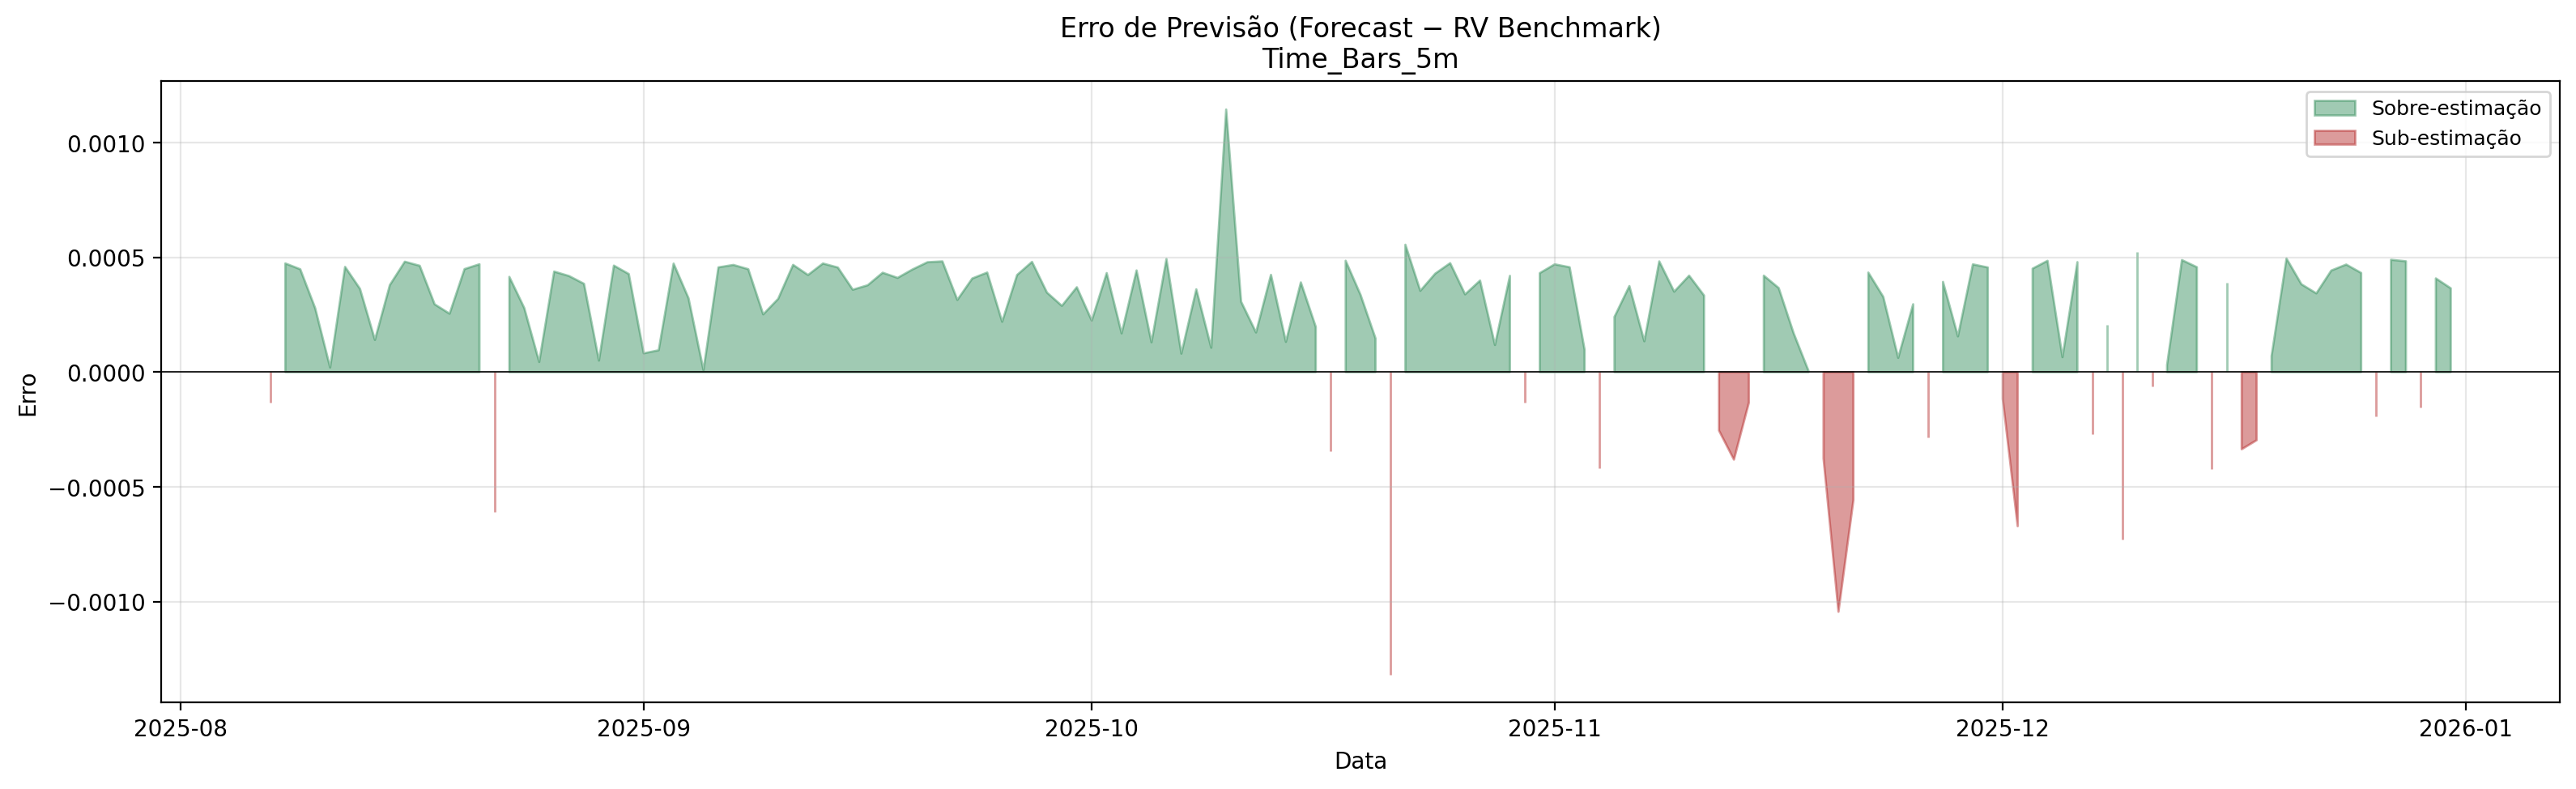
\includegraphics[width=\textwidth]{analise_previsao/Time_Bars_5m/Time_Bars_5m_02_erro_previsao.png}
        \subcaption{Erros de previsão.}
        \label{fig:prev_time_erro}
    \end{minipage}
    \caption{Previsão da variância condicional versus variância realizada (TSRV) --- \emph{Time Bars} GARCH(1,1), período de teste (07/ago/2025--31/dez/2025).}
    \label{fig:prev_time_grid}
\end{figure}


% -----------------------------------------------------------------------------
\subsection{Análise de Resíduos}
\label{subsec:analise_residuos}

A análise de resíduos do modelo ajustado constitui um diagnóstico
essencial para verificar se os modelos GARCH estimados capturam
adequadamente a estrutura de dependência das séries de retornos.
Avalia-se, em particular, se os resíduos padronizados apresentam
ausência de autocorrelação serial, distribuição aproximadamente
normal e ausência de efeitos ARCH remanescentes.

% --------------------------------------------------

\begin{figure}[H]
    \centering
    \begin{minipage}[t]{0.48\textwidth}
        \centering
        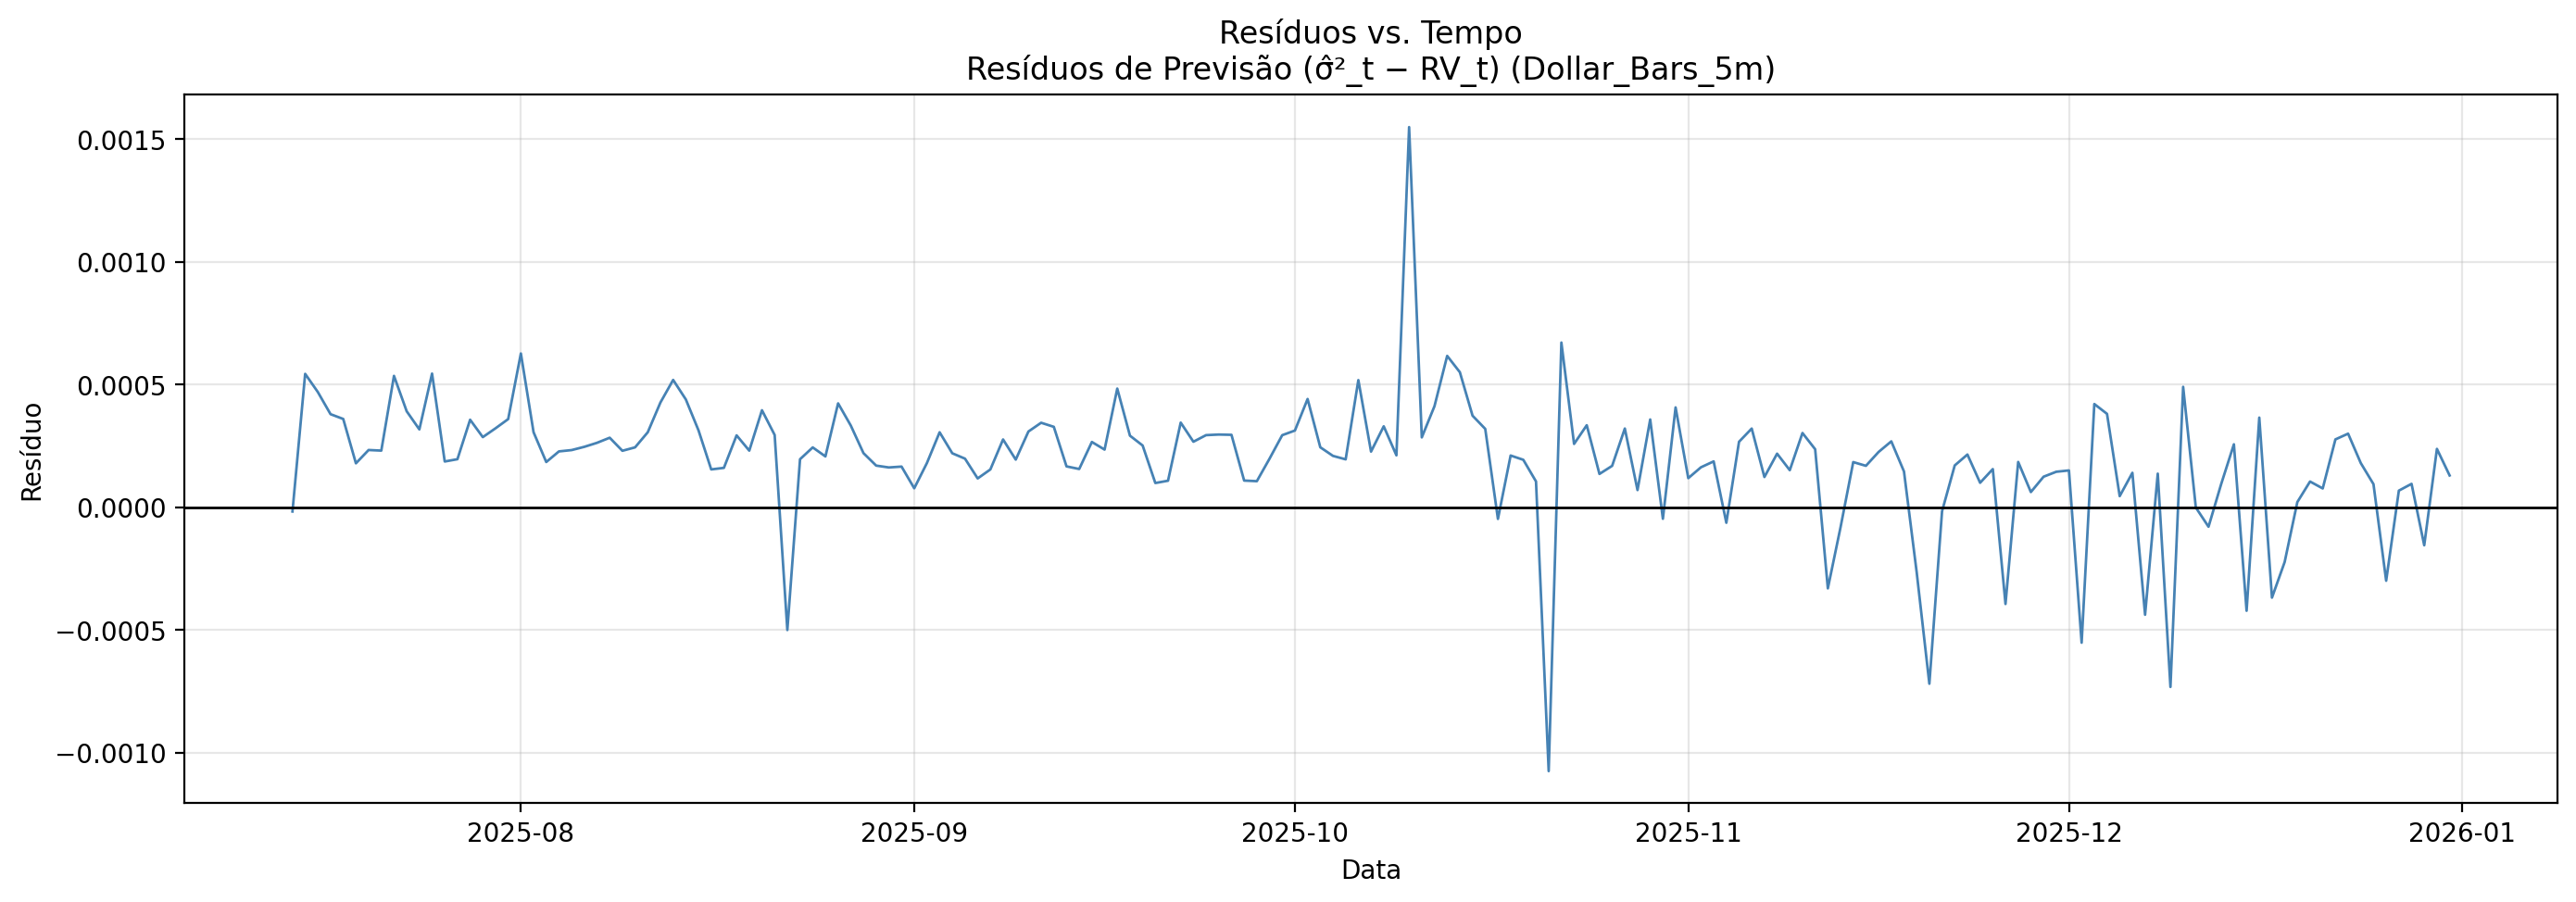
\includegraphics[width=\textwidth]{analise_residuos/Dollar_Bars_5m/forecast_errors_Dollar_Bars_5m_01_residuos_tempo.png}
        \subcaption{Resíduos padronizados ao longo do tempo.}
        \label{fig:res_dollar_tempo}
    \end{minipage}
    \hfill
    \begin{minipage}[t]{0.48\textwidth}
        \centering
        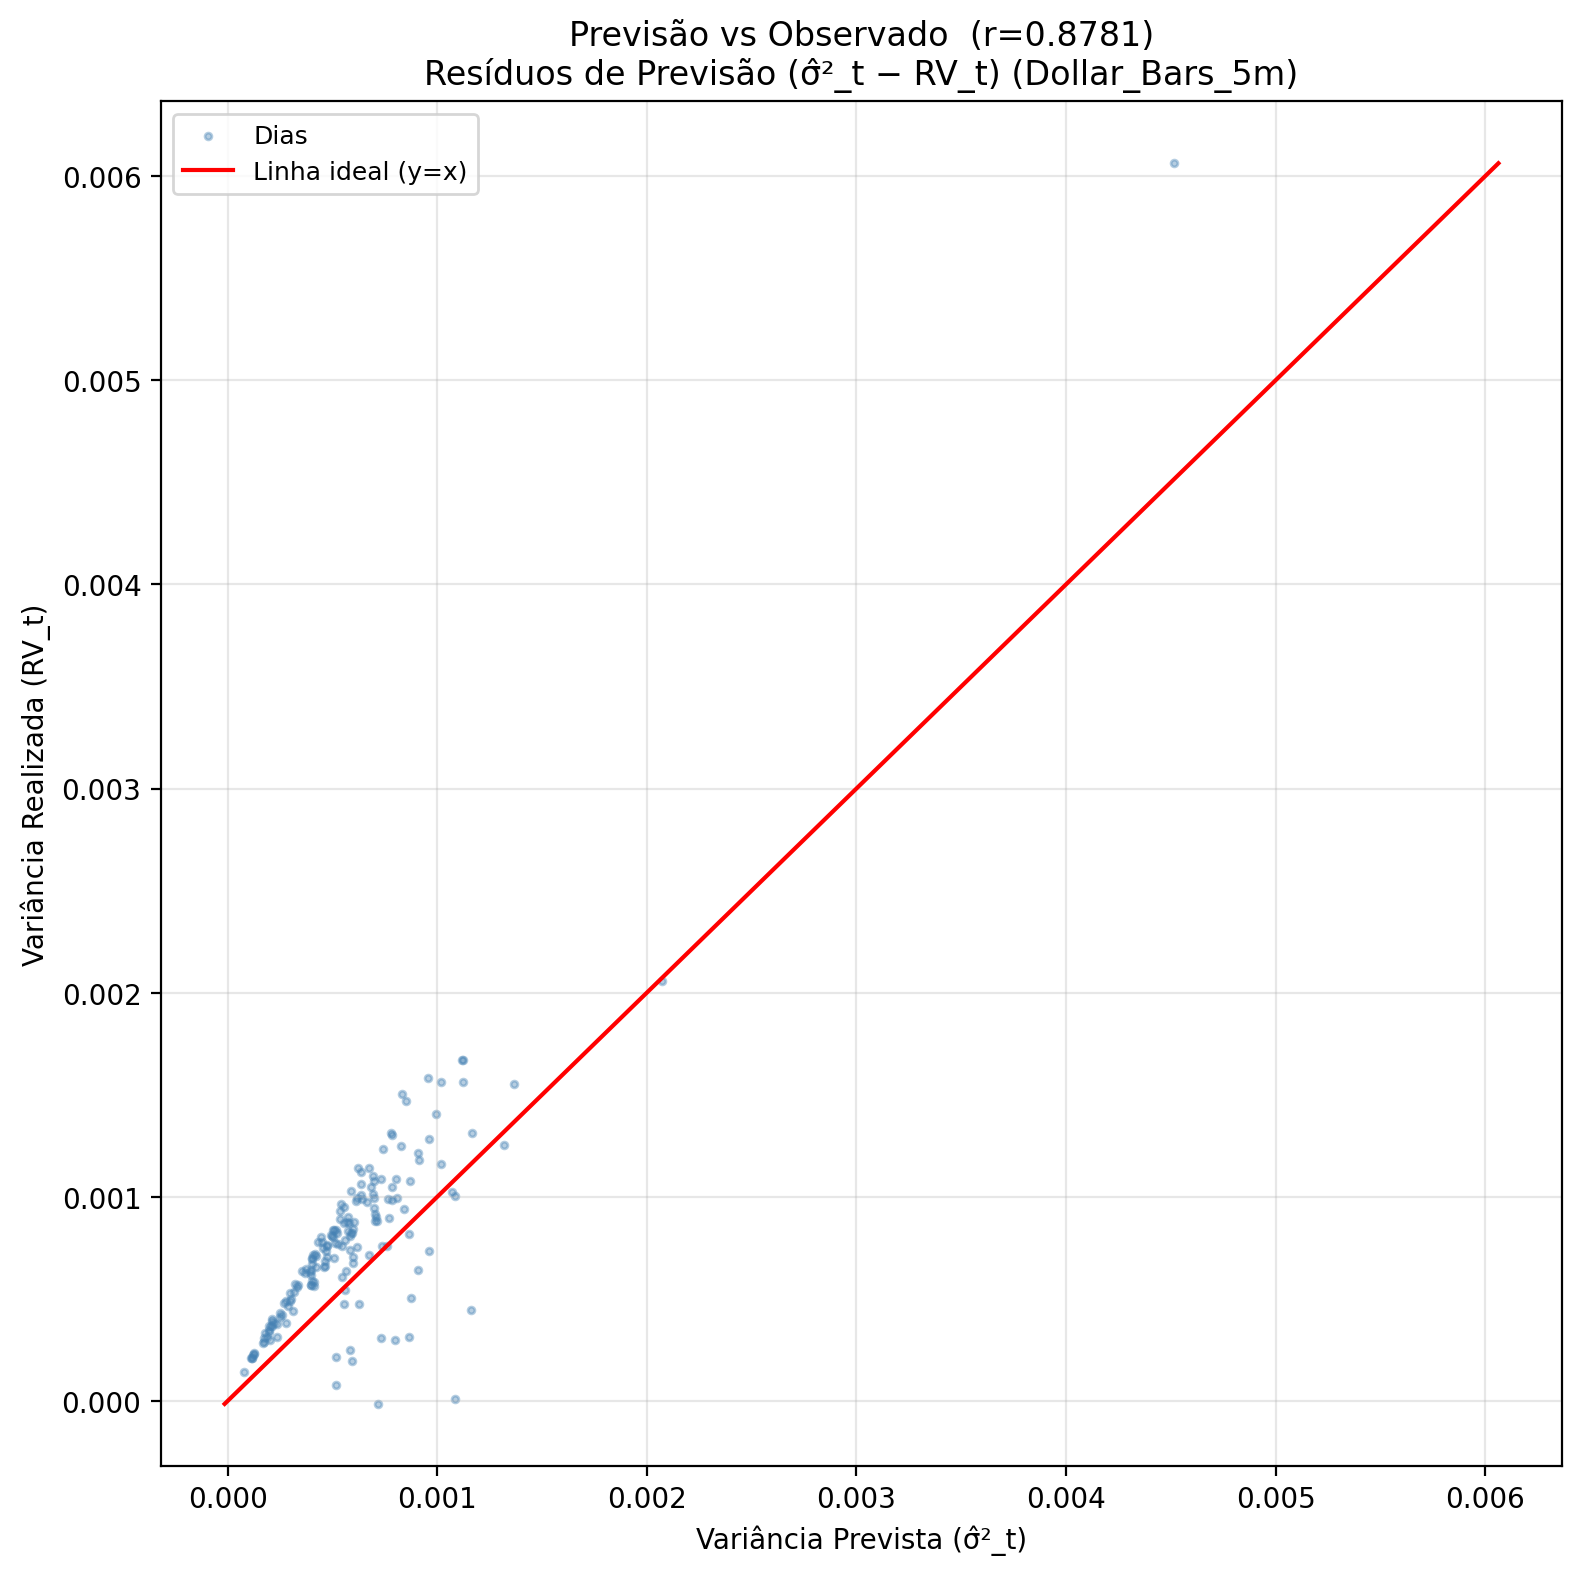
\includegraphics[width=\textwidth]{analise_residuos/Dollar_Bars_5m/forecast_errors_Dollar_Bars_5m_08_previsao_vs_observado.png}
        \subcaption{Previsão versus variância realizada (TSRV).}
        \label{fig:res_dollar_previsao_obs}
    \end{minipage}
    
    \vspace{0.5cm}
    \begin{minipage}[t]{0.48\textwidth}
        \centering
        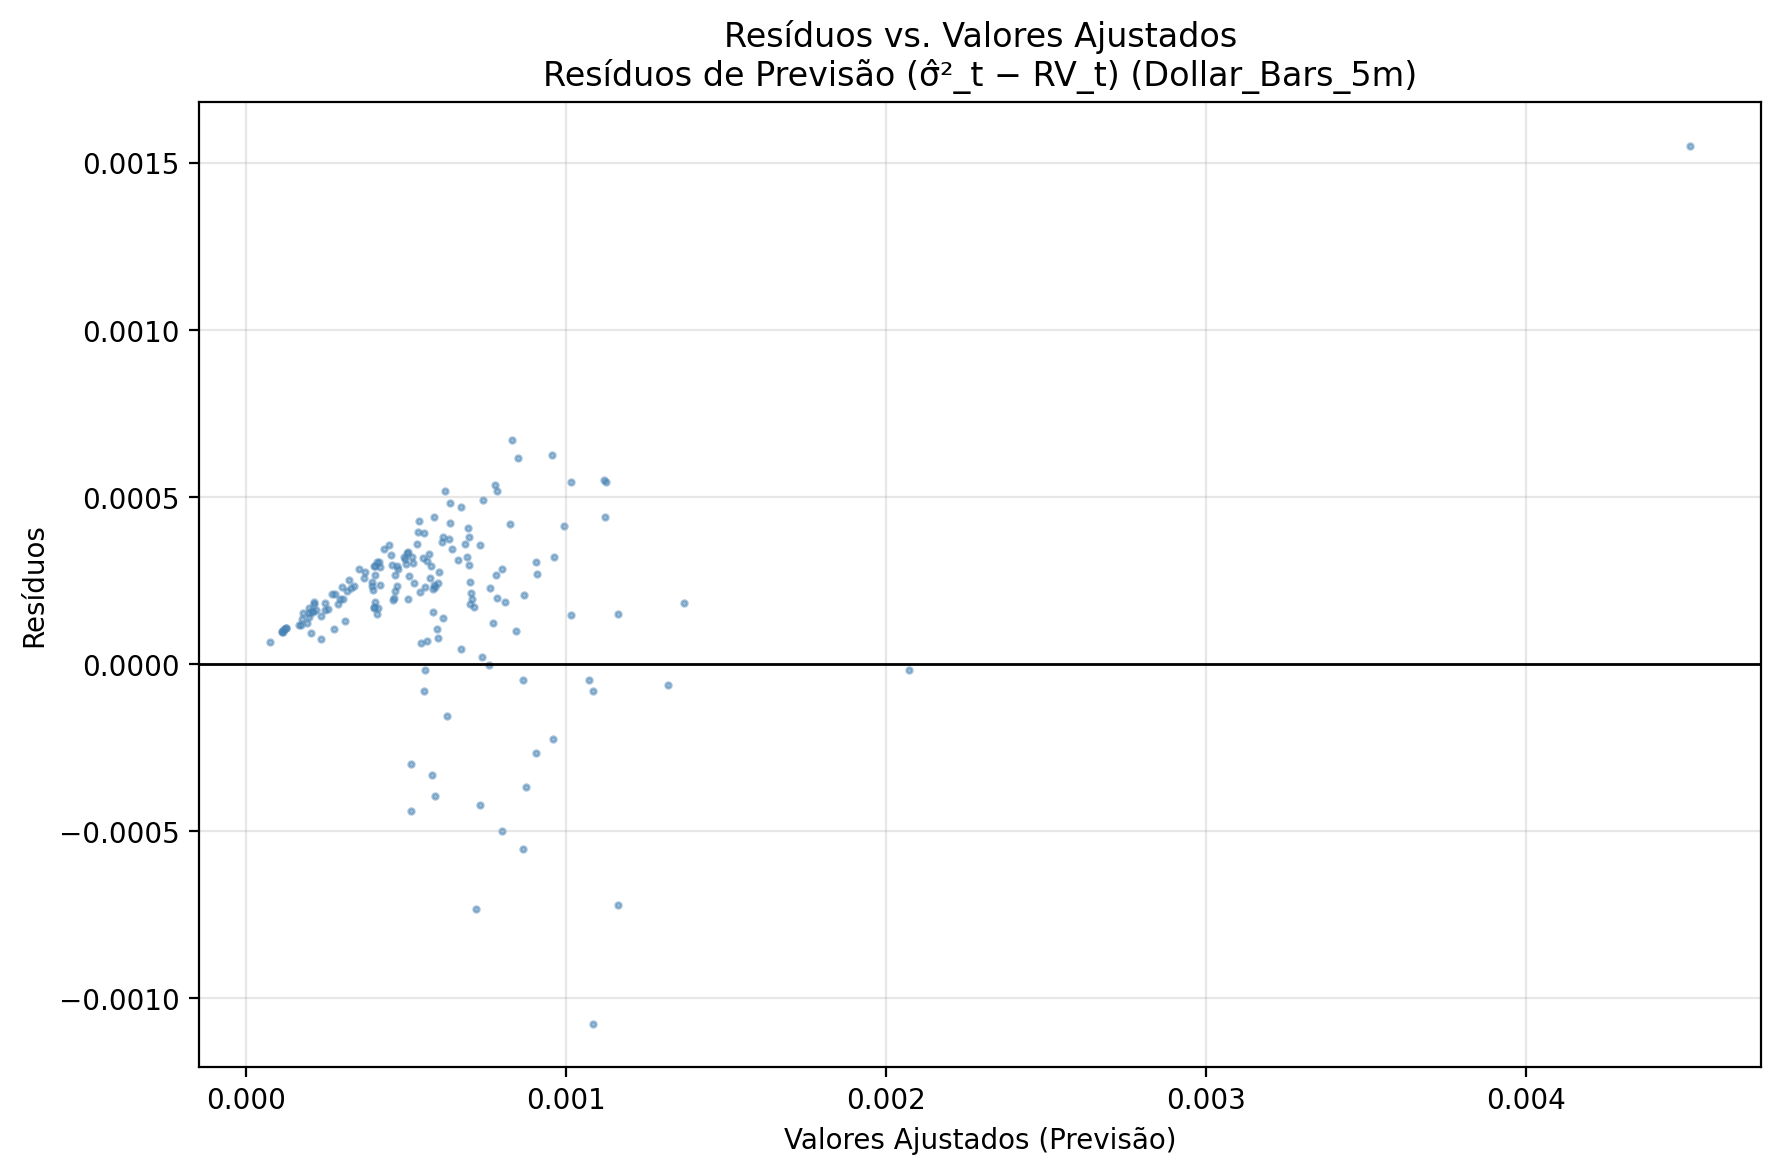
\includegraphics[width=\textwidth]{analise_residuos/Dollar_Bars_5m/forecast_errors_Dollar_Bars_5m_04_residuos_vs_ajustados.png}
        \subcaption{Resíduos versus valores ajustados.}
        \label{fig:res_dollar_vs_ajust}
    \end{minipage}
    \hfill
    \begin{minipage}[t]{0.48\textwidth}
        \centering
        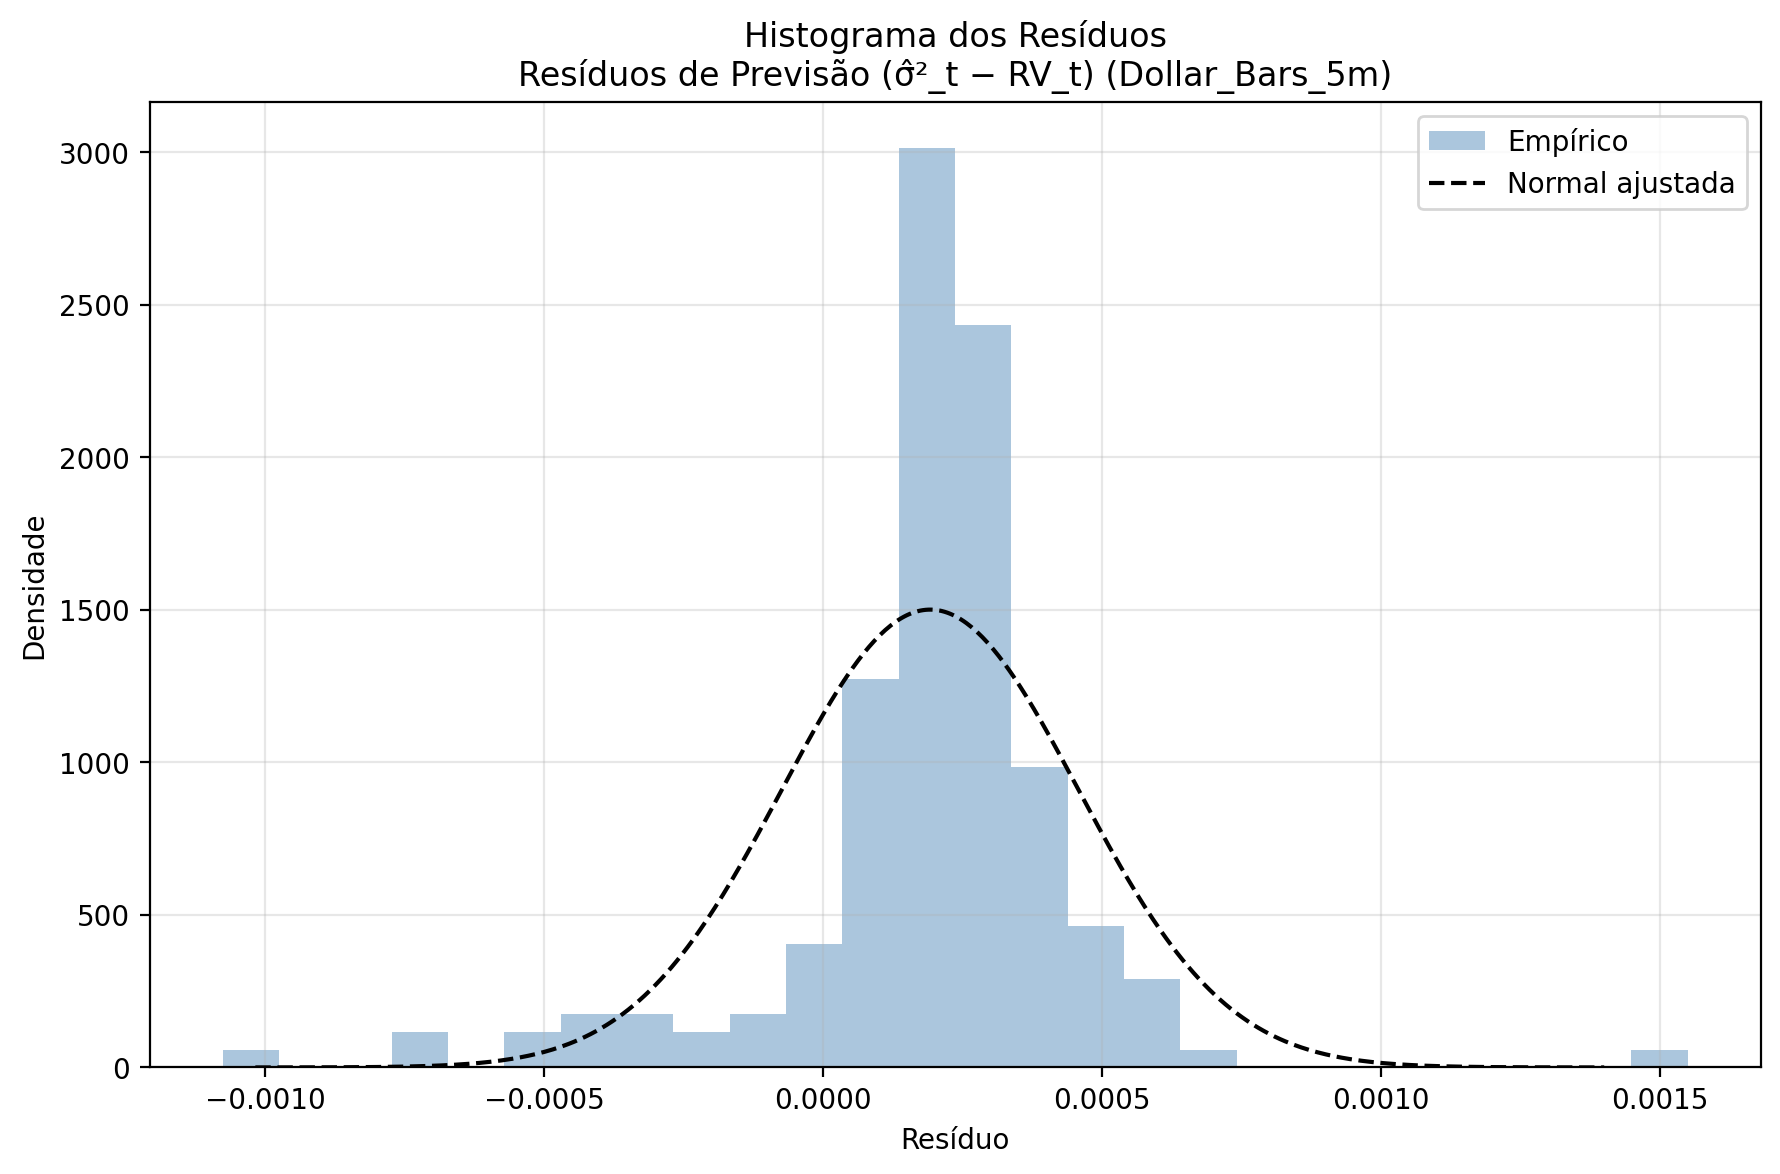
\includegraphics[width=\textwidth]{analise_residuos/Dollar_Bars_5m/forecast_errors_Dollar_Bars_5m_02_histograma.png}
        \subcaption{Histograma com curva normal sobreposta.}
        \label{fig:res_dollar_hist}
    \end{minipage}
    \caption{Diagnósticos de ajuste e distribuição dos resíduos --- \emph{Dollar Bars} GARCH(1,2).}
    \label{fig:res_dollar_grid1}
\end{figure}

\begin{figure}[H]
    \centering
    \begin{minipage}[t]{0.48\textwidth}
        \centering
        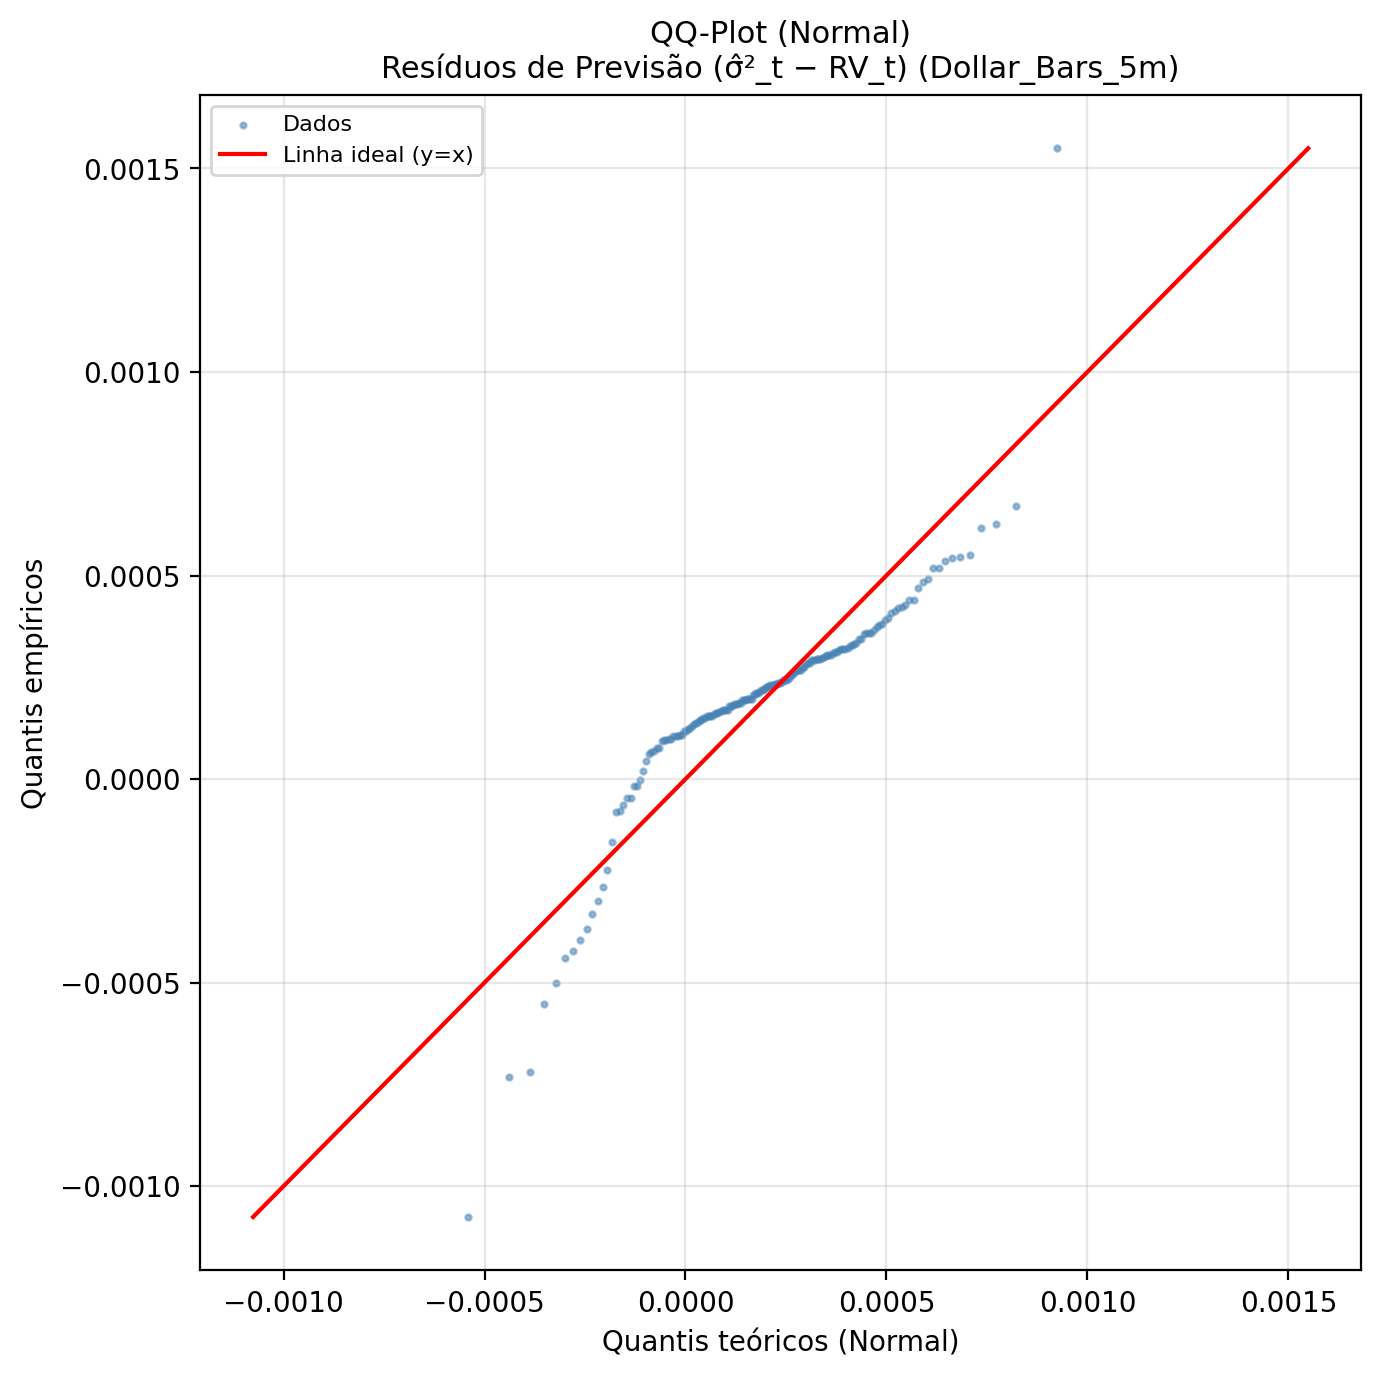
\includegraphics[width=\textwidth]{analise_residuos/Dollar_Bars_5m/forecast_errors_Dollar_Bars_5m_03_qqplot_normal.png}
        \subcaption{QQ-Plot versus distribuição normal.}
        \label{fig:res_dollar_qq}
    \end{minipage}
    \hfill
    \begin{minipage}[t]{0.48\textwidth}
        \centering
        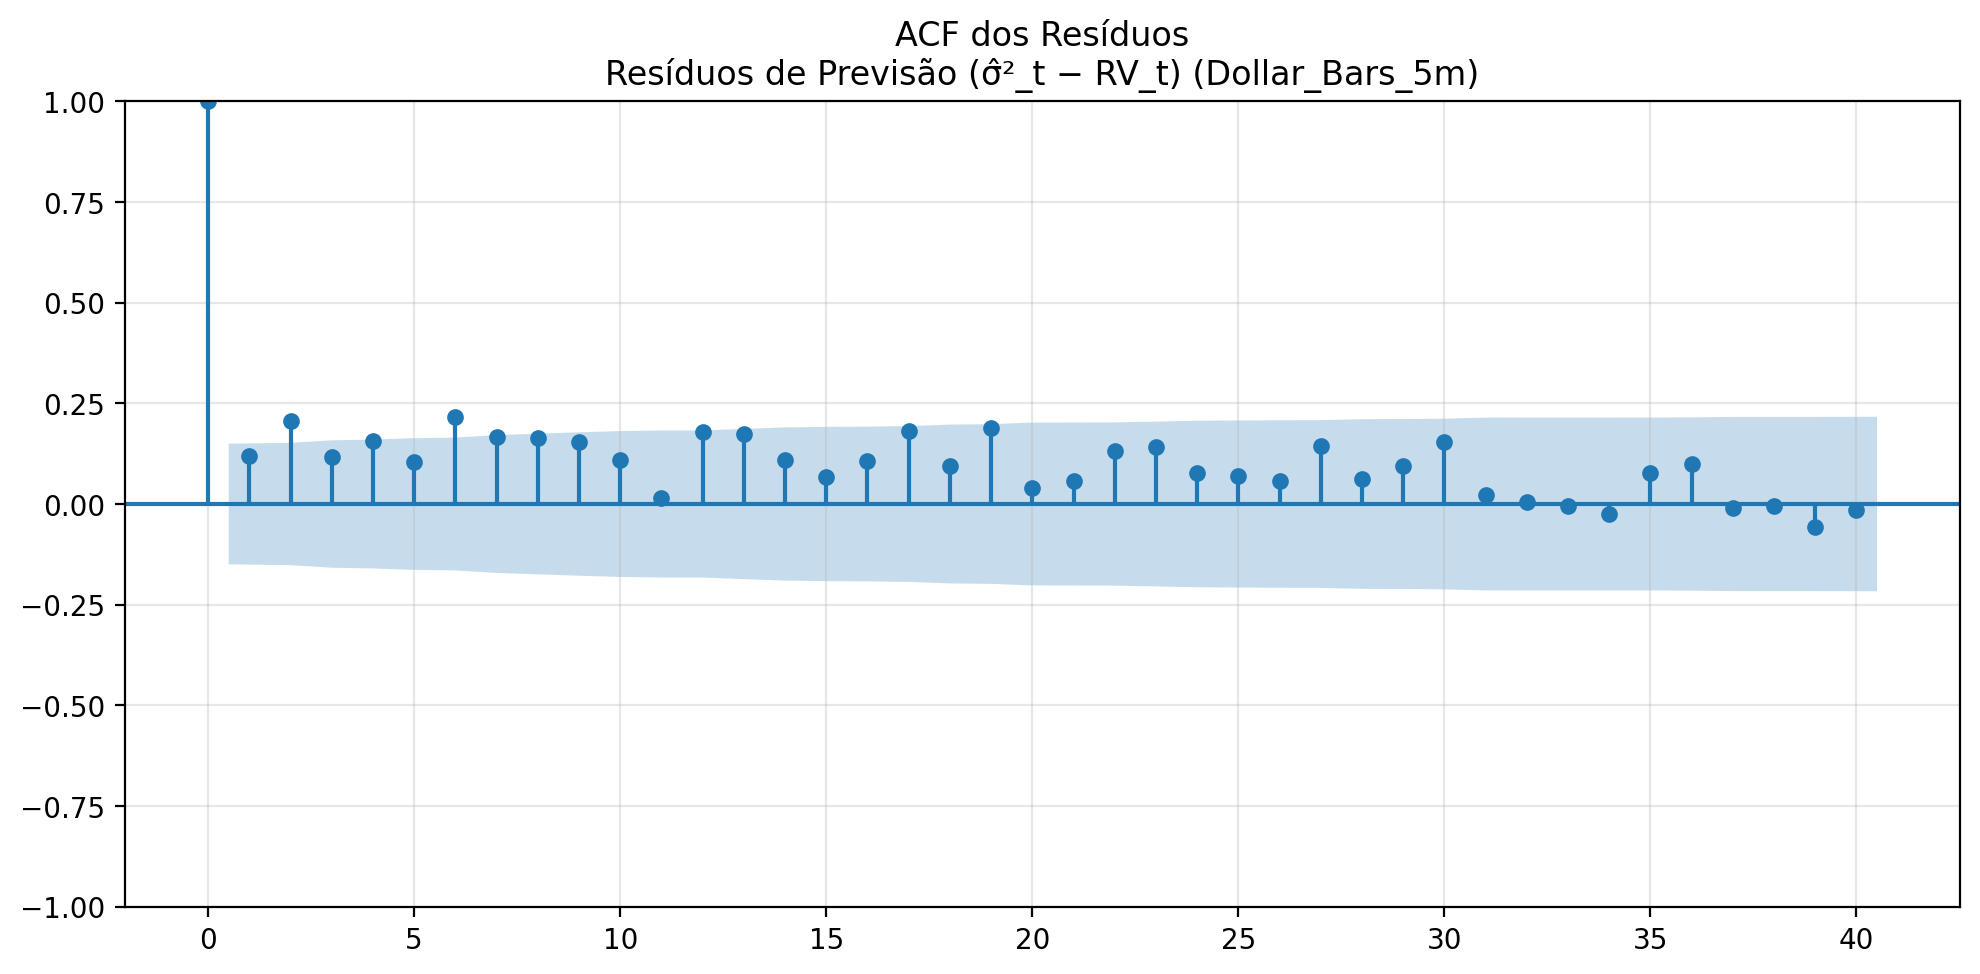
\includegraphics[width=\textwidth]{analise_residuos/Dollar_Bars_5m/forecast_errors_Dollar_Bars_5m_05_acf_residuos.png}
        \subcaption{Função de Autocorrelação (FAC).}
        \label{fig:res_dollar_acf}
    \end{minipage}
    
    \vspace{0.5cm}
    \begin{minipage}[t]{0.48\textwidth}
        \centering
        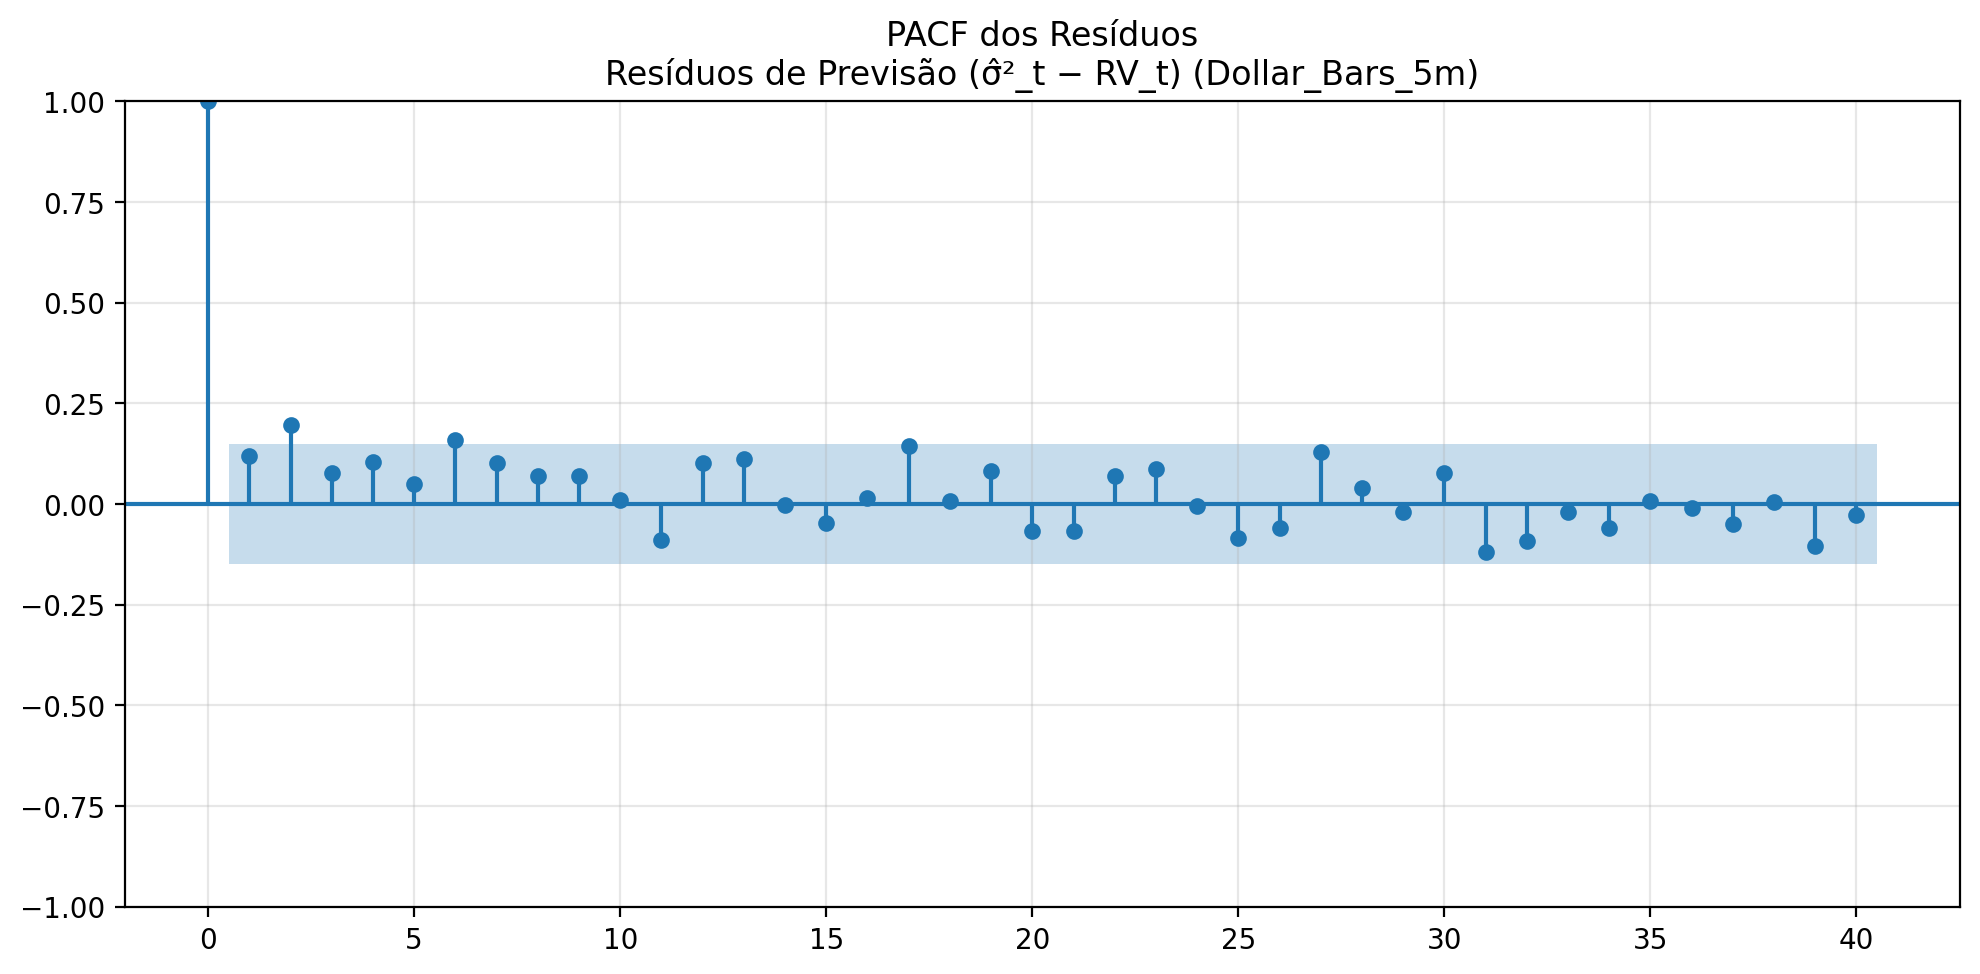
\includegraphics[width=\textwidth]{analise_residuos/Dollar_Bars_5m/forecast_errors_Dollar_Bars_5m_06_pacf_residuos.png}
        \subcaption{Função de Autocorrelação Parcial (FACP).}
        \label{fig:res_dollar_pacf}
    \end{minipage}
    \hfill
    \begin{minipage}[t]{0.48\textwidth}
        \centering
        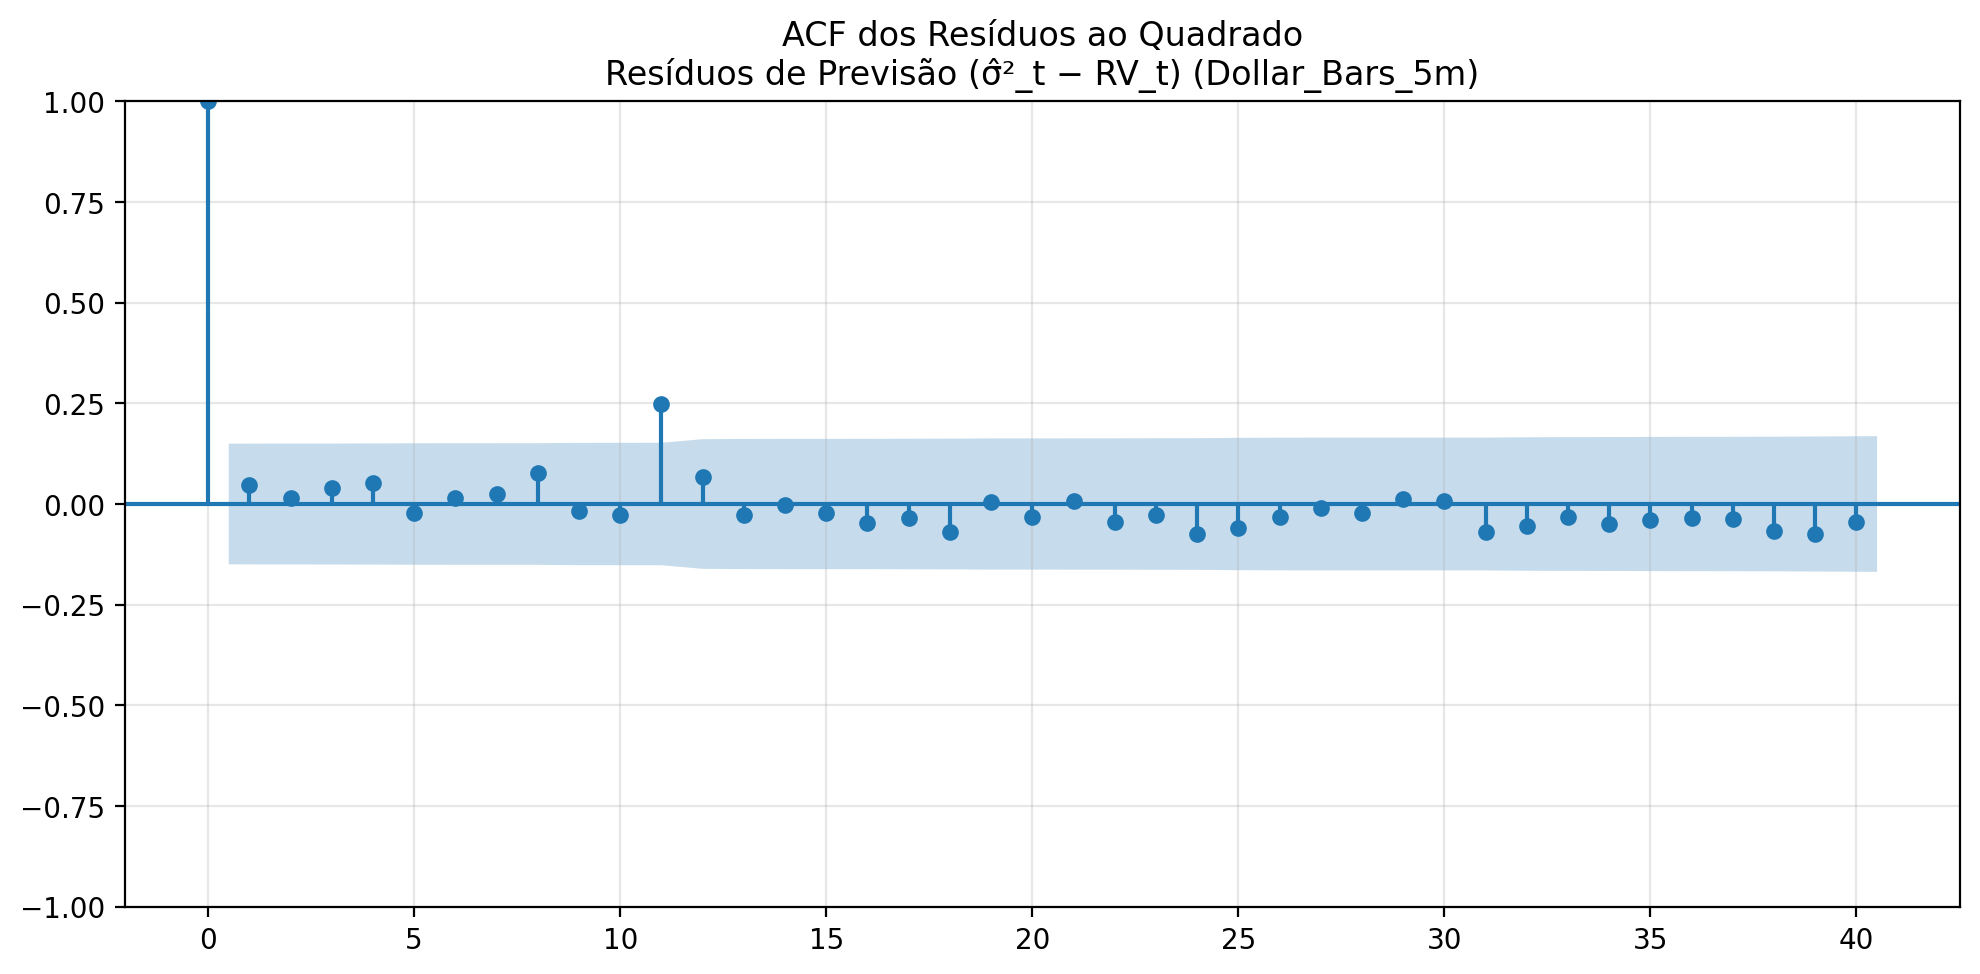
\includegraphics[width=\textwidth]{analise_residuos/Dollar_Bars_5m/forecast_errors_Dollar_Bars_5m_07_acf_residuos_quadrado.png}
        \subcaption{FAC dos resíduos ao quadrado.}
        \label{fig:res_dollar_acf_sq}
    \end{minipage}
    \caption{Diagnósticos de normalidade e dependência --- \emph{Dollar Bars} GARCH(1,2).}
    \label{fig:res_dollar_grid2}
\end{figure}

A análise gráfica dos resíduos padronizados do modelo ajustado sobre as \emph{dollar bars} (Figuras \ref{fig:res_dollar_grid1} e \ref{fig:res_dollar_grid2}) permite avaliar a adequação do GARCH(1,2) sob três aspectos principais: estabilidade temporal, distribuição dos erros e dependência serial.

Com relação à estabilidade temporal e o ajuste geral (\autoref{fig:res_dollar_grid1}), observa-se que os resíduos padronizados (a) distribuem-se de maneira razoavelmente homogênea ao redor de zero, sem apresentar agrupamentos prolongados de alta variância não contabilizada. A dispersão da previsão versus a variância realizada (b) e contra os valores ajustados (c) evidencia a capacidade do modelo em acompanhar a trajetória da volatilidade (TSRV), porém indicando tendência (viés sistemático) em suas previsões. Por fim, o histograma (d) sobreposto à curva normal demonstra como a distribuição empírica dos erros se comporta em relação à distribuição Gaussiana assumida pela Máxima Verossimilhança.

Essa divergência em relação à normalidade é mais claramente constatada nos diagnósticos da \autoref{fig:res_dollar_grid2}. O QQ-Plot (a) revela desvios notáveis nas caudas da distribuição teórica, um indicativo clássico de caudas pesadas (leptocurtose) comum a retornos financeiros, o qual persiste mesmo após a filtragem GARCH. Apesar dos desvios distribucionais nas extremidades, os filtros mostraram-se competentes na remoção da dependência serial: as Funções de Autocorrelação (FAC) e Autocorrelação Parcial (FACP) dos resíduos (b e c) apresentam coeficientes majoritariamente contidos no interior do intervalo de confiança de 95\%, corroborando a adequação da equação da média. Fundamentalmente, a FAC dos resíduos ao quadrado (d) opera como o diagnóstico de efeitos ARCH remanescentes. A ausência de autocorrelações significativas fora das faixas azuis assegura que a estrutura GARCH(1,2) capturou adequadamente a dinâmica de \textit{volatility clustering}, absorvendo a dependência não-linear da série de maneira eficaz.

% --------------------------------------------------

\begin{figure}[H]
    \centering
    \begin{minipage}[t]{0.48\textwidth}
        \centering
        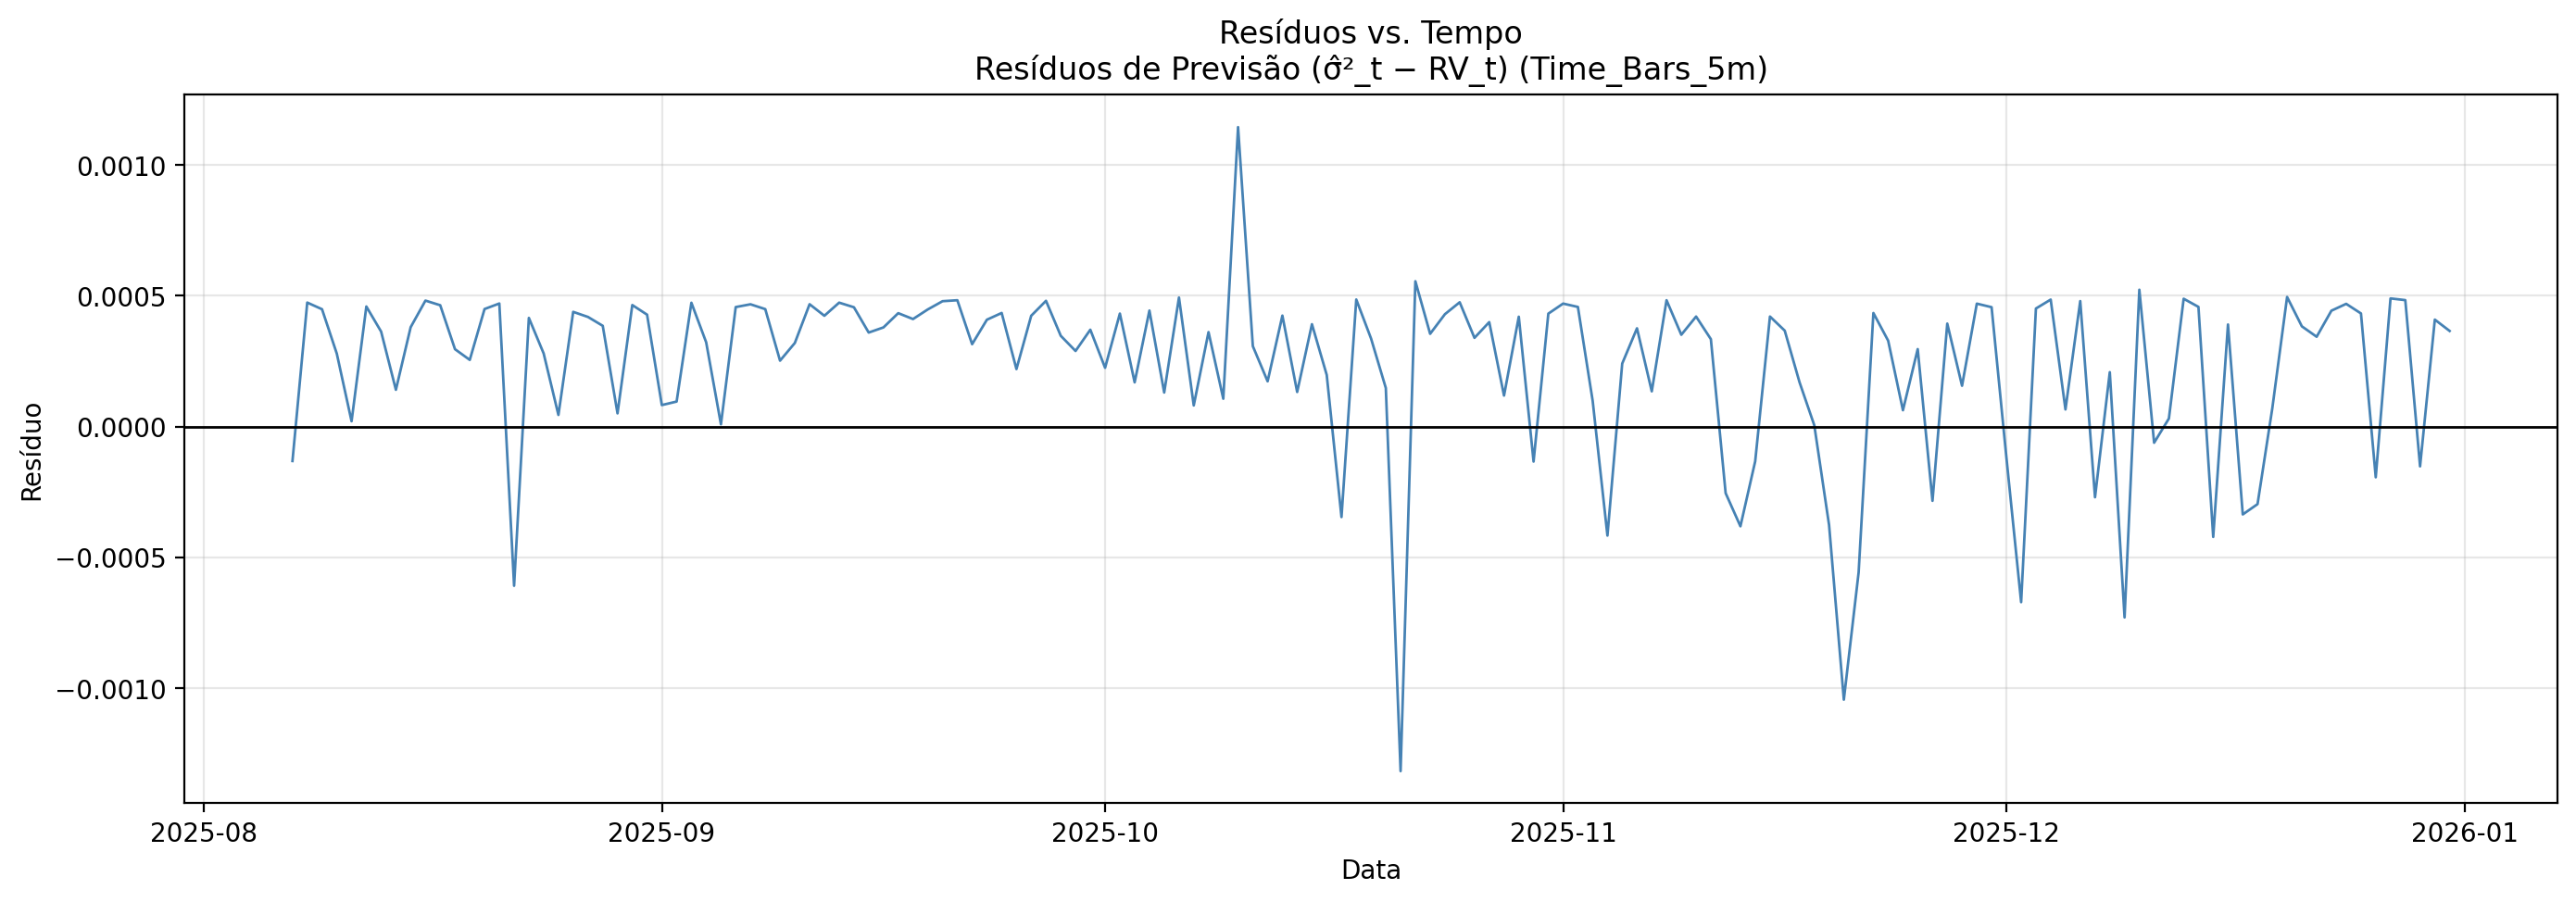
\includegraphics[width=\textwidth]{analise_residuos/Time_Bars_5m/forecast_errors_Time_Bars_5m_01_residuos_tempo.png}
        \subcaption{Resíduos padronizados ao longo do tempo.}
        \label{fig:res_time_tempo}
    \end{minipage}
    \hfill
    \begin{minipage}[t]{0.48\textwidth}
        \centering
        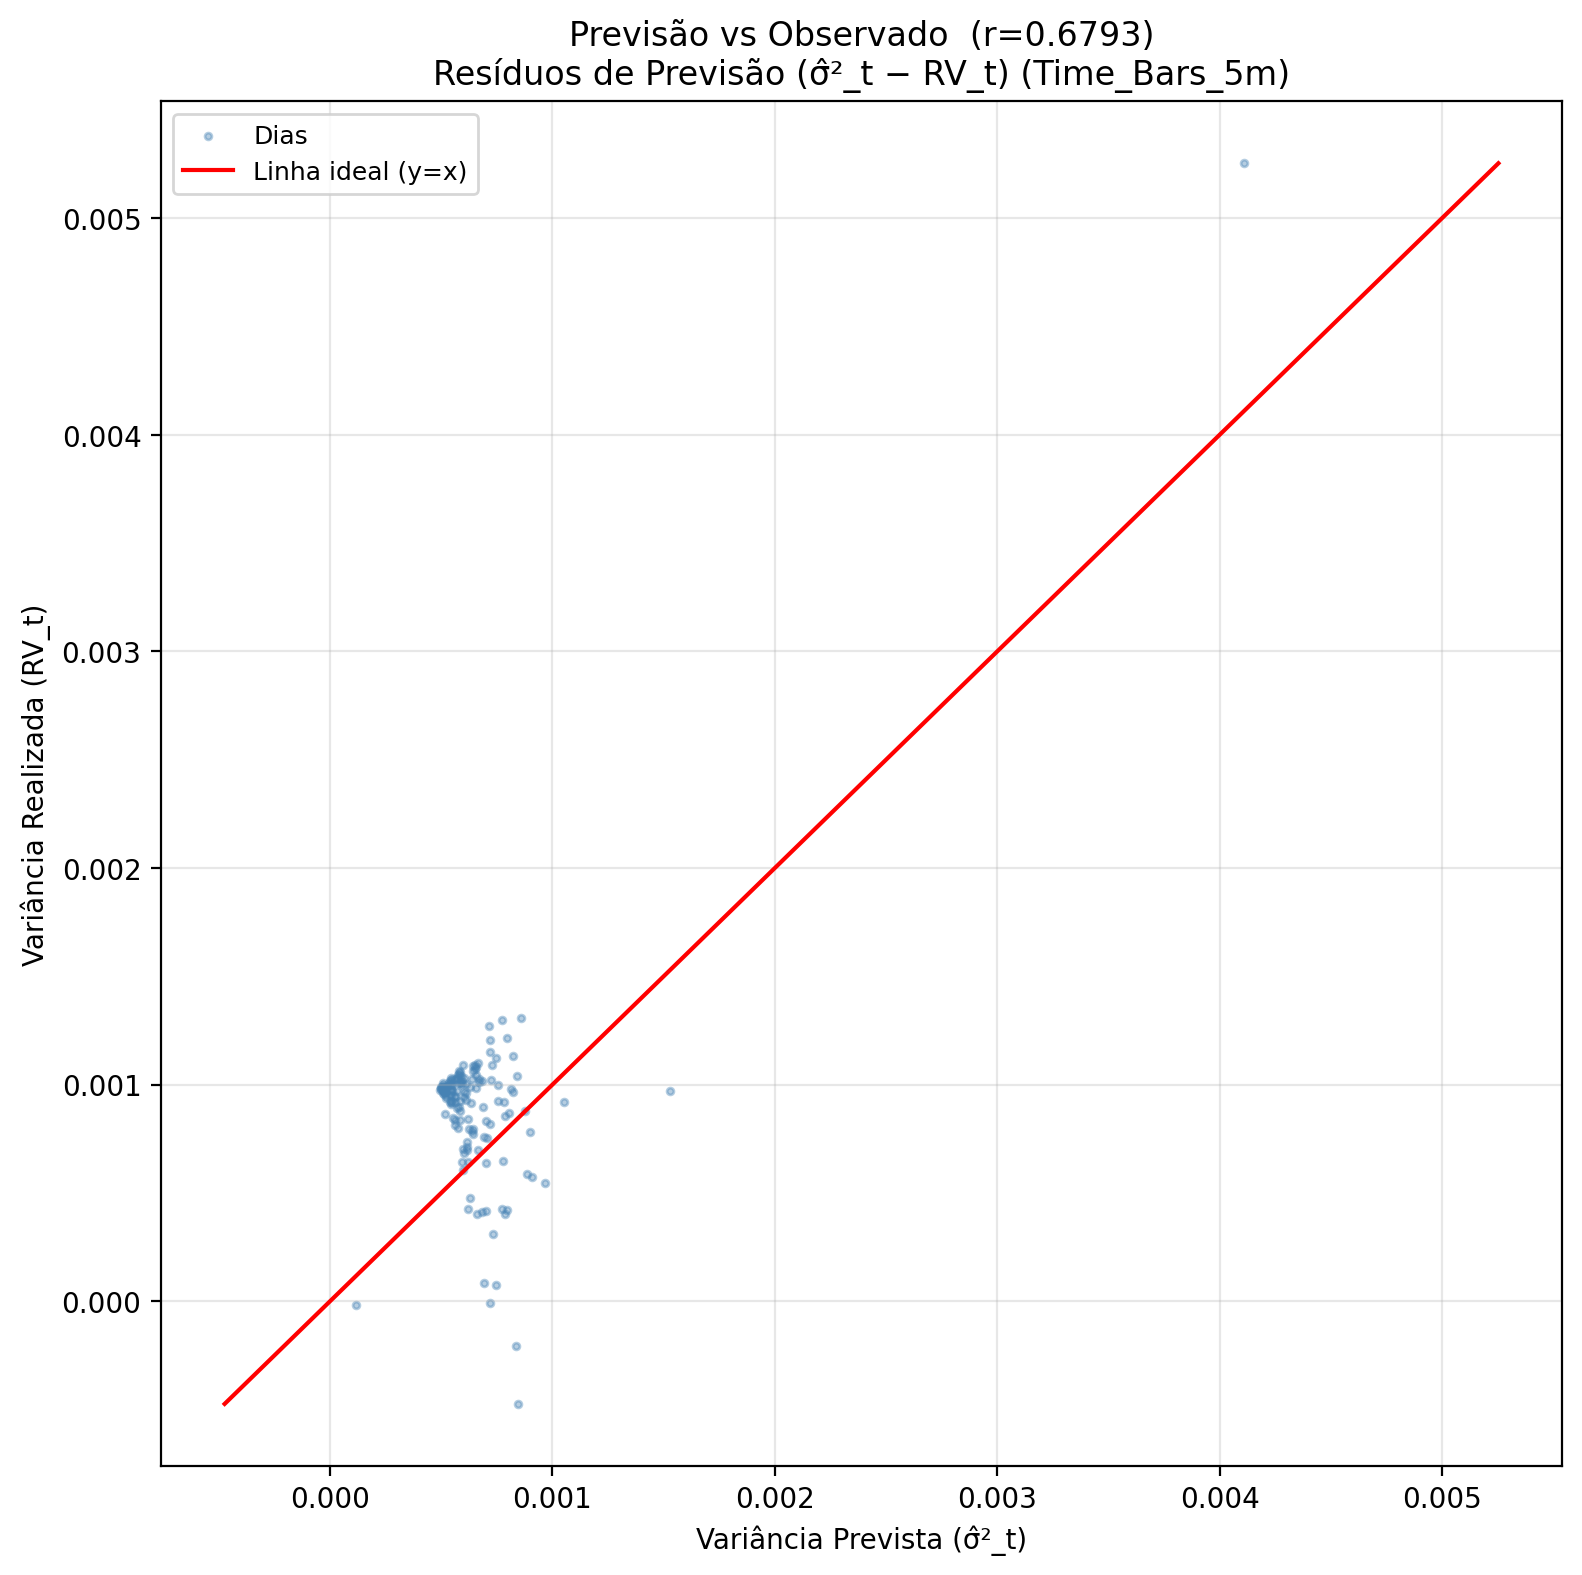
\includegraphics[width=\textwidth]{analise_residuos/Time_Bars_5m/forecast_errors_Time_Bars_5m_08_previsao_vs_observado.png}
        \subcaption{Previsão versus variância realizada (TSRV).}
        \label{fig:res_time_previsao_obs}
    \end{minipage}
    
    \vspace{0.5cm}
    \begin{minipage}[t]{0.48\textwidth}
        \centering
        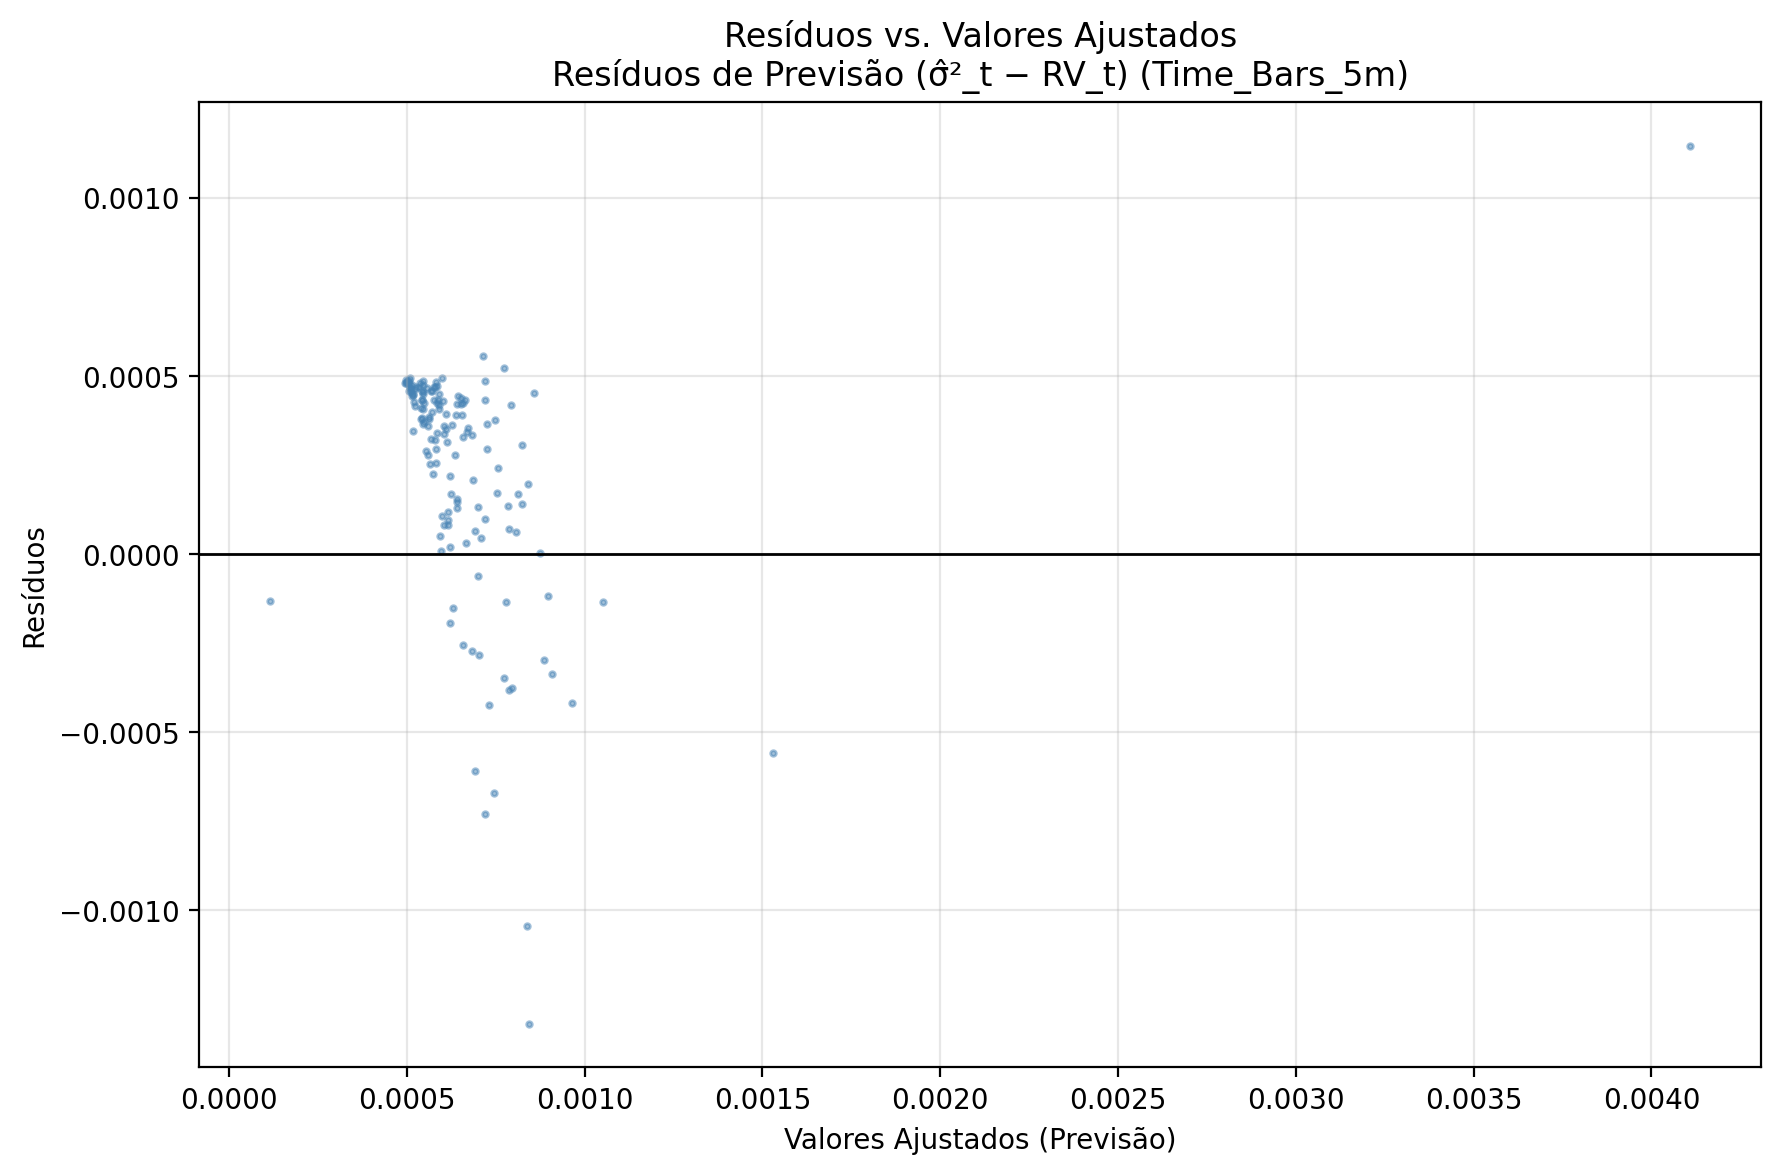
\includegraphics[width=\textwidth]{analise_residuos/Time_Bars_5m/forecast_errors_Time_Bars_5m_04_residuos_vs_ajustados.png}
        \subcaption{Resíduos versus valores ajustados.}
        \label{fig:res_time_vs_ajust}
    \end{minipage}
    \hfill
    \begin{minipage}[t]{0.48\textwidth}
        \centering
        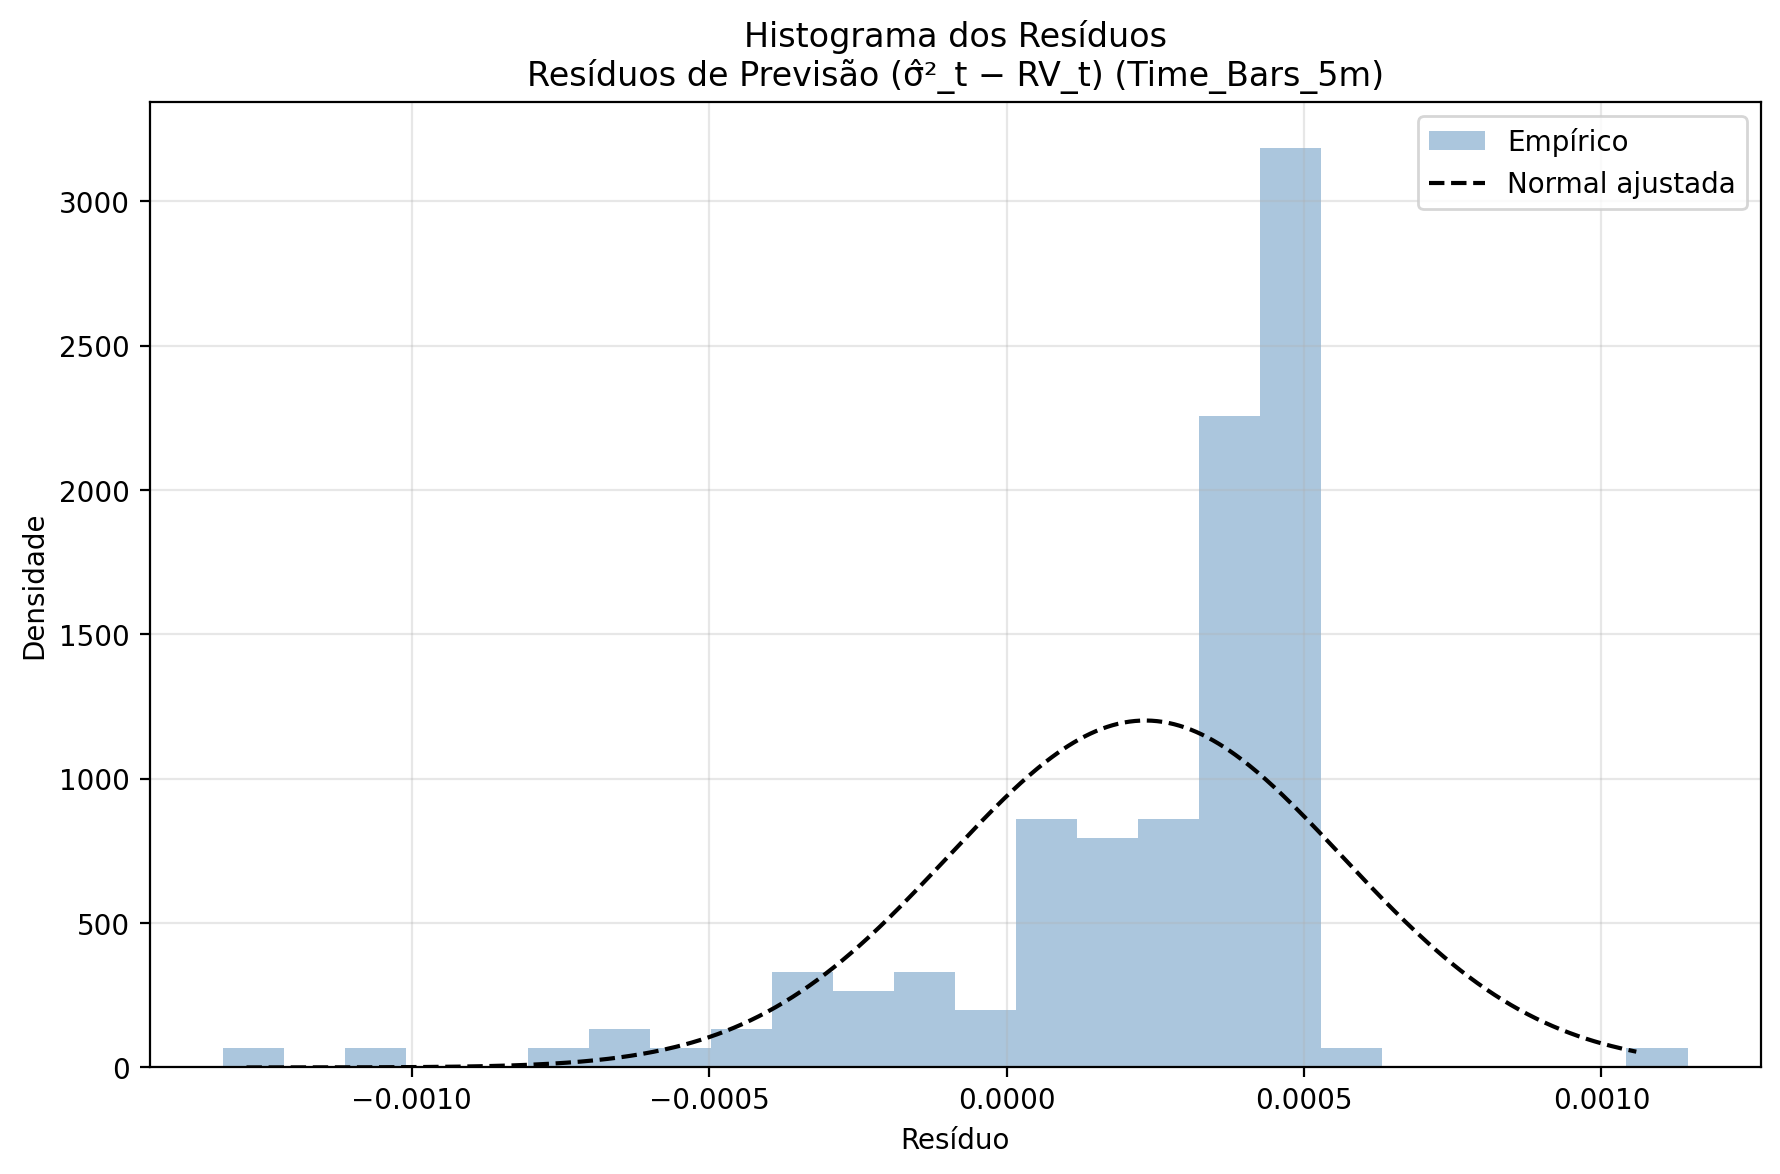
\includegraphics[width=\textwidth]{analise_residuos/Time_Bars_5m/forecast_errors_Time_Bars_5m_02_histograma.png}
        \subcaption{Histograma com curva normal sobreposta.}
        \label{fig:res_time_hist}
    \end{minipage}
    \caption{Diagnósticos de ajuste e distribuição dos resíduos --- \emph{Time Bars} GARCH(1,1).}
    \label{fig:res_time_grid1}
\end{figure}

\begin{figure}[H]
    \centering
    \begin{minipage}[t]{0.48\textwidth}
        \centering
        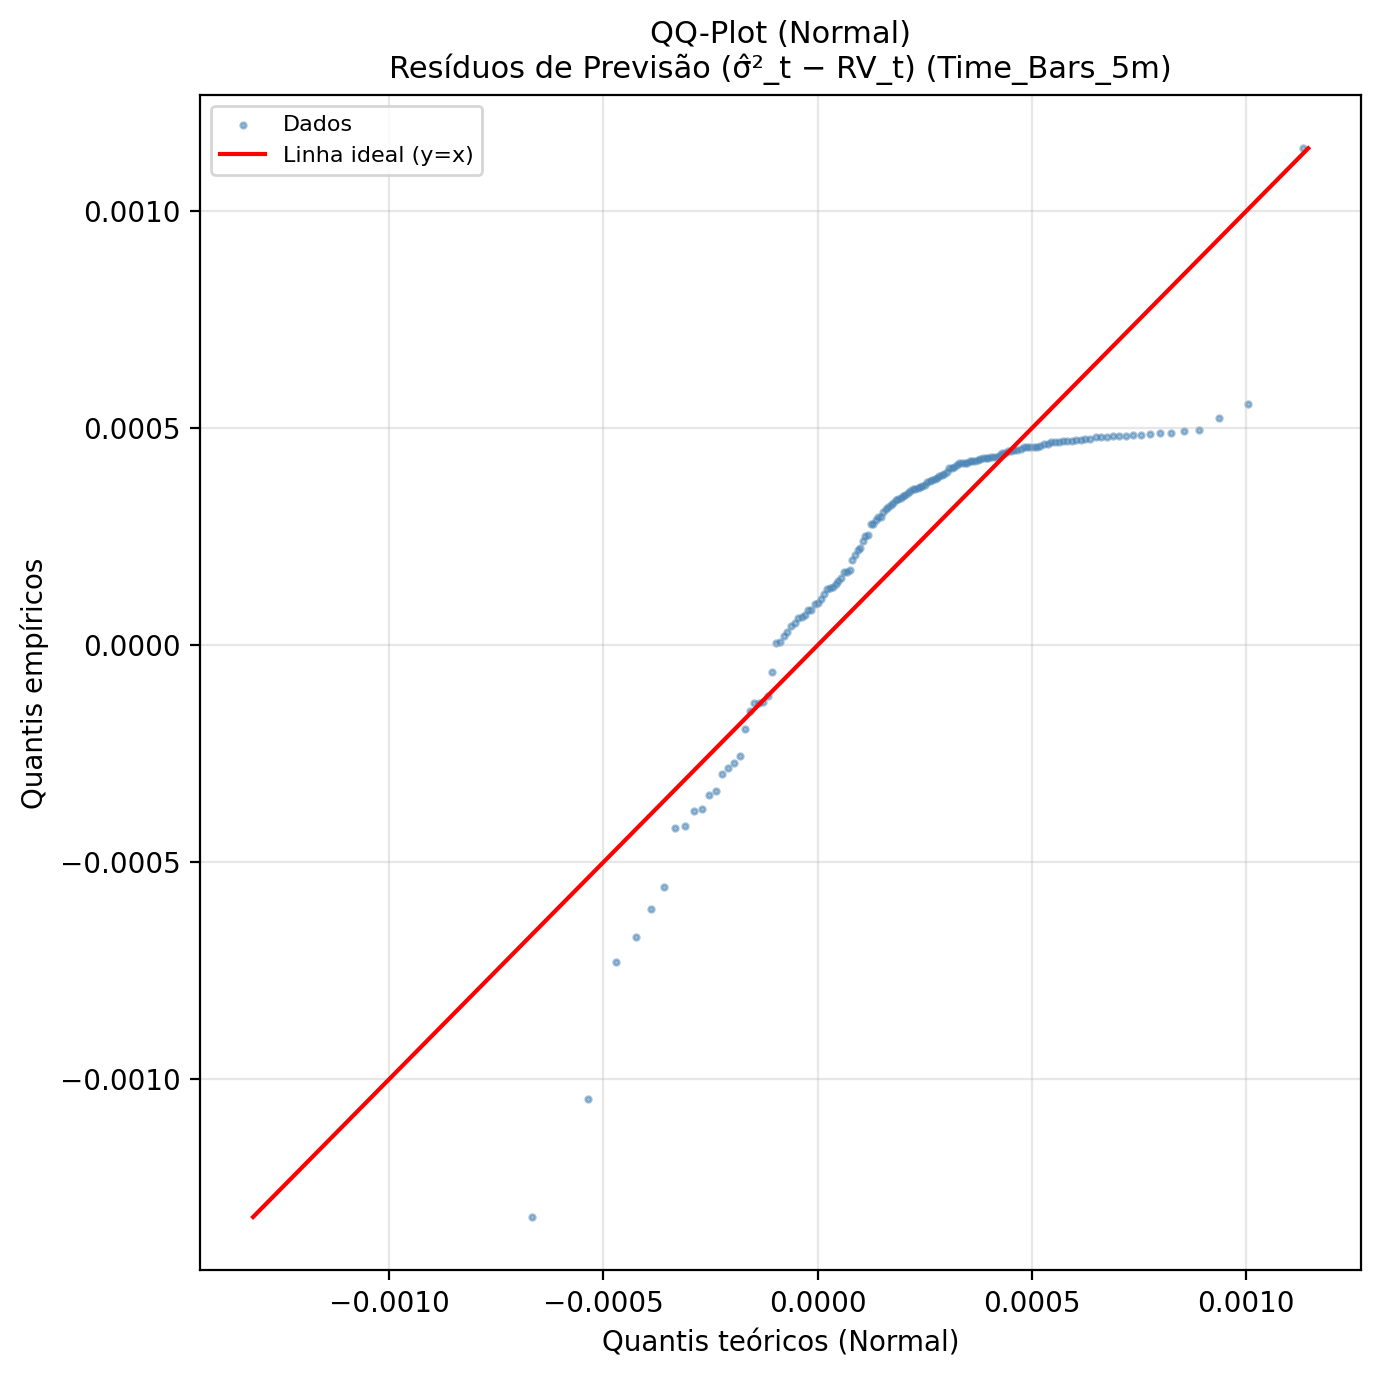
\includegraphics[width=\textwidth]{analise_residuos/Time_Bars_5m/forecast_errors_Time_Bars_5m_03_qqplot_normal.png}
        \subcaption{QQ-Plot versus distribuição normal.}
        \label{fig:res_time_qq}
    \end{minipage}
    \hfill
    \begin{minipage}[t]{0.48\textwidth}
        \centering
        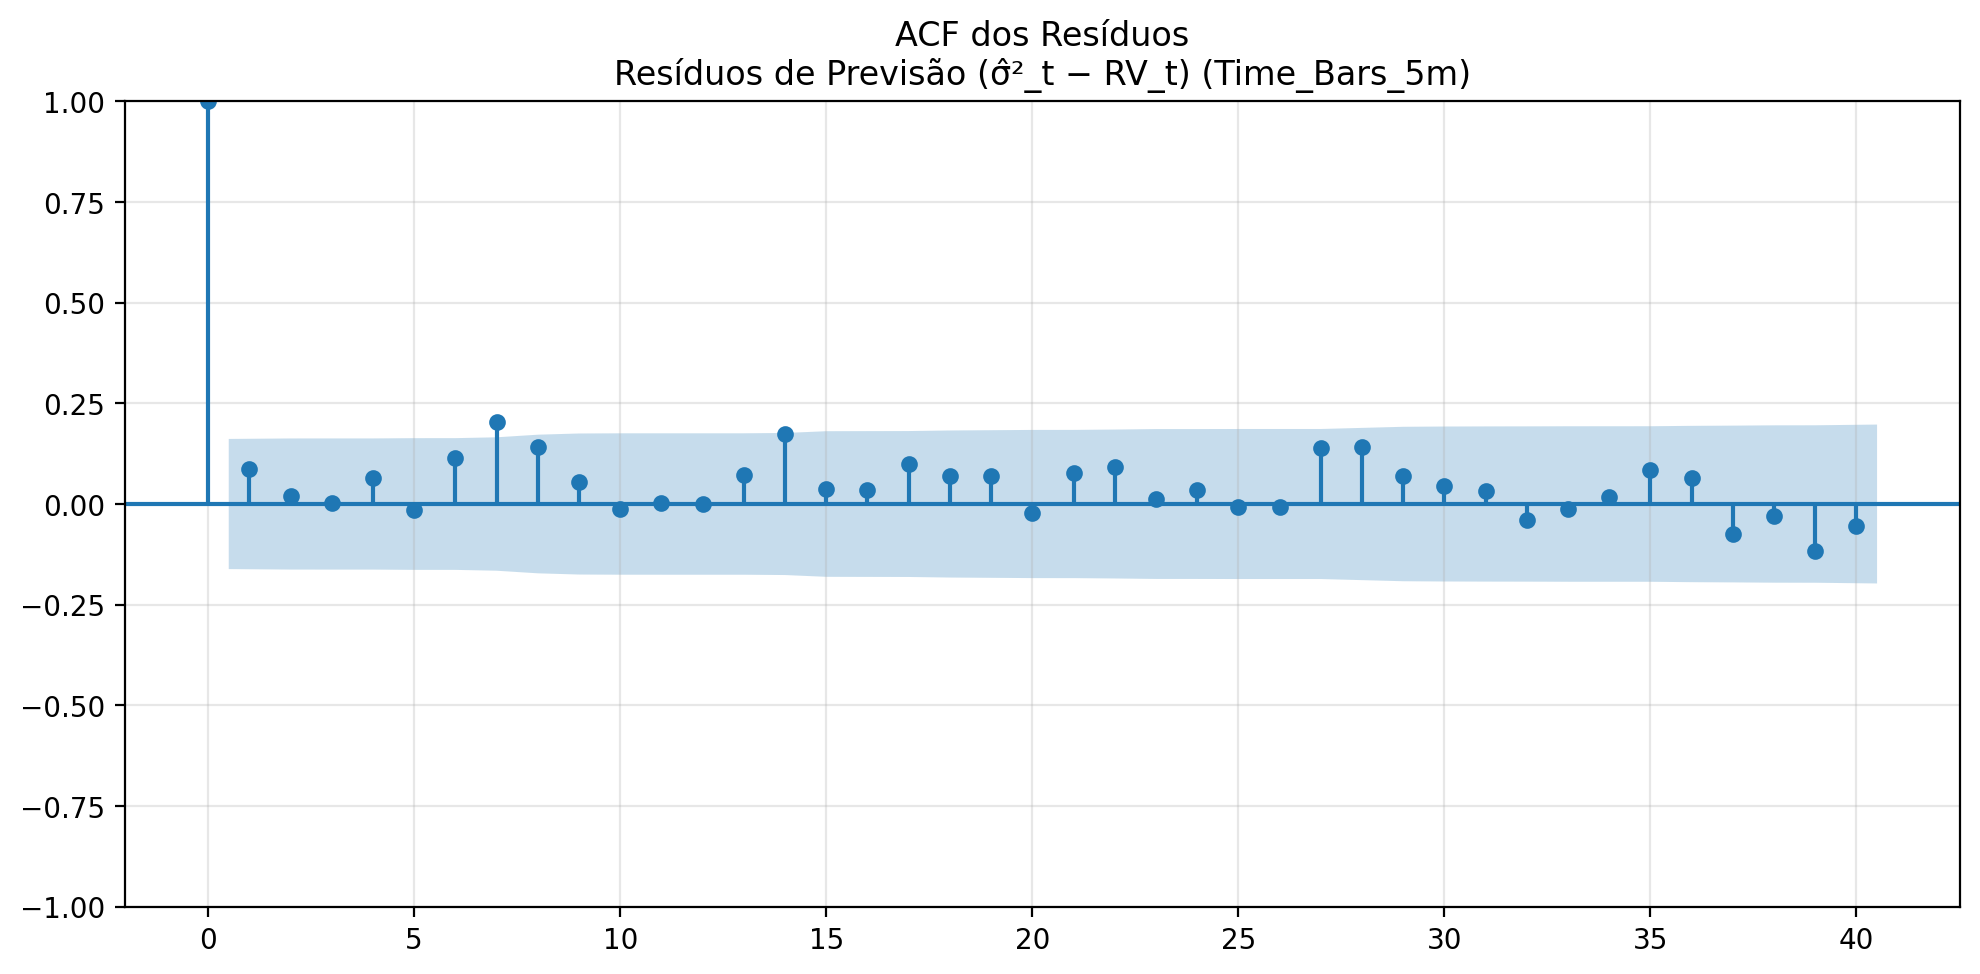
\includegraphics[width=\textwidth]{analise_residuos/Time_Bars_5m/forecast_errors_Time_Bars_5m_05_acf_residuos.png}
        \subcaption{Função de Autocorrelação (FAC).}
        \label{fig:res_time_acf}
    \end{minipage}
    
    \vspace{0.5cm}
    \begin{minipage}[t]{0.48\textwidth}
        \centering
        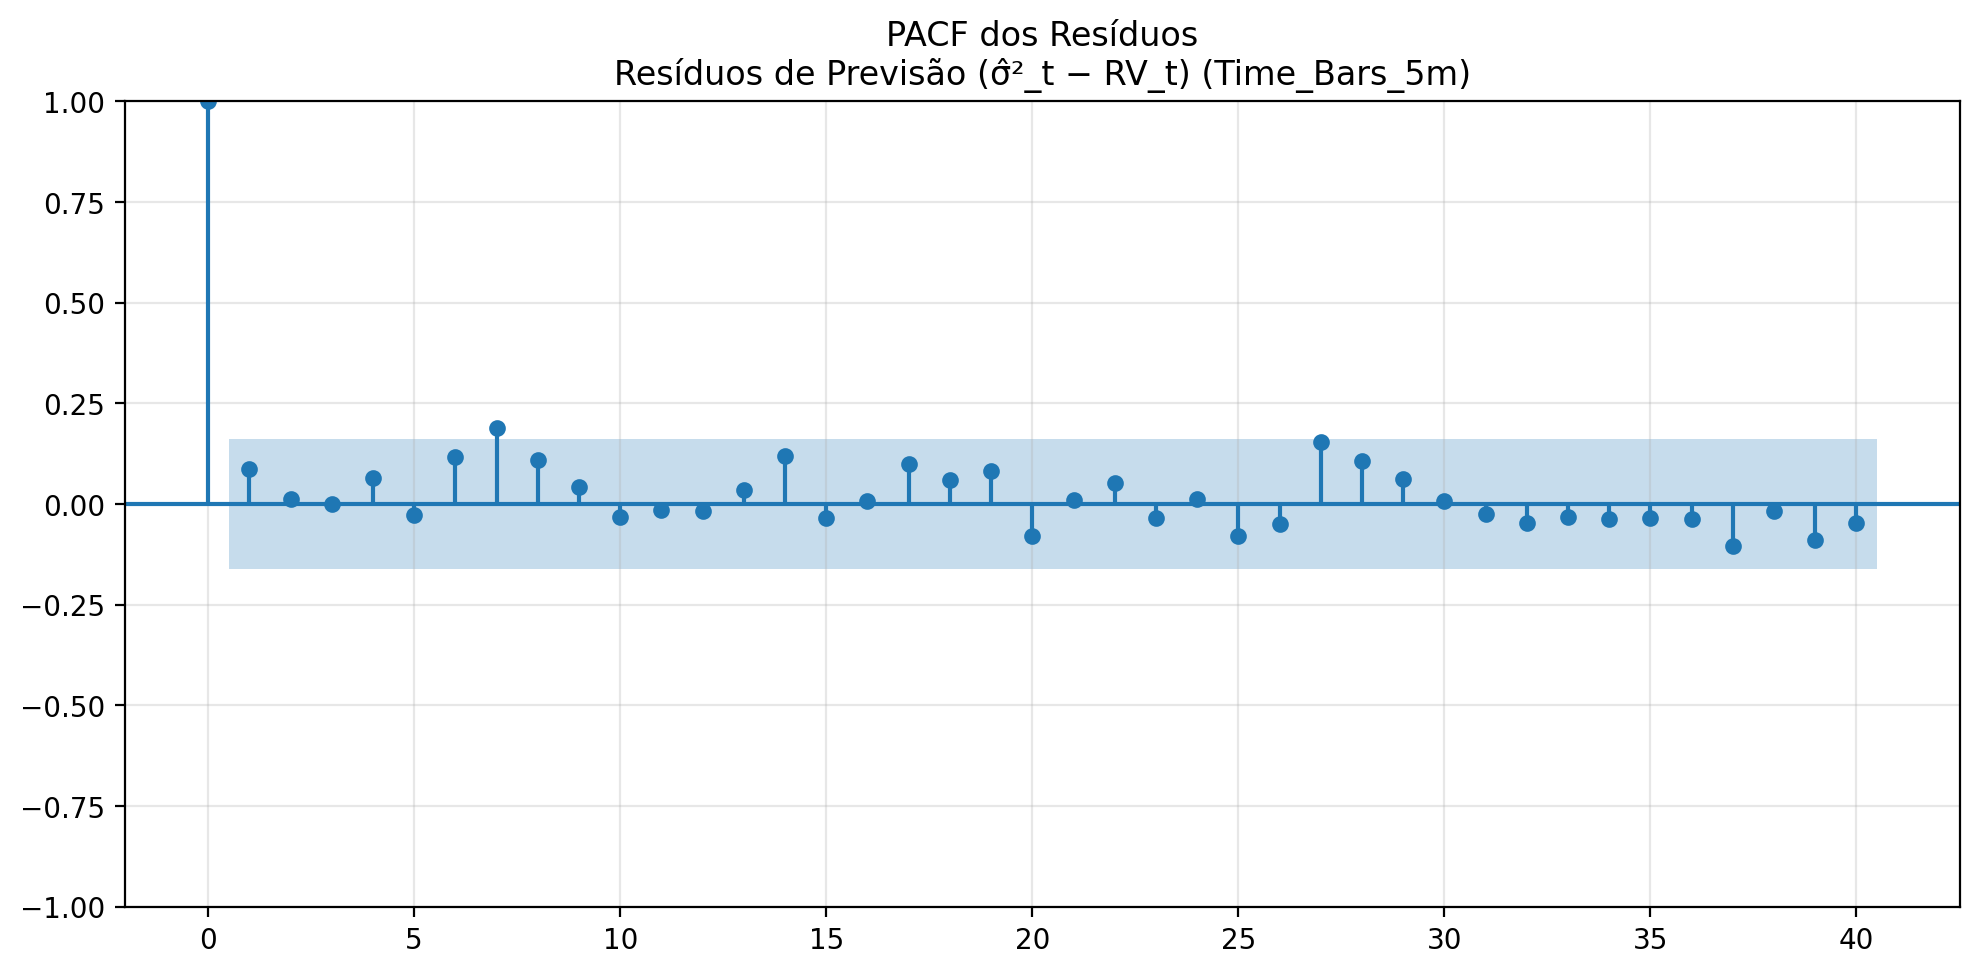
\includegraphics[width=\textwidth]{analise_residuos/Time_Bars_5m/forecast_errors_Time_Bars_5m_06_pacf_residuos.png}
        \subcaption{Função de Autocorrelação Parcial (FACP).}
        \label{fig:res_time_pacf}
    \end{minipage}
    \hfill
    \begin{minipage}[t]{0.48\textwidth}
        \centering
        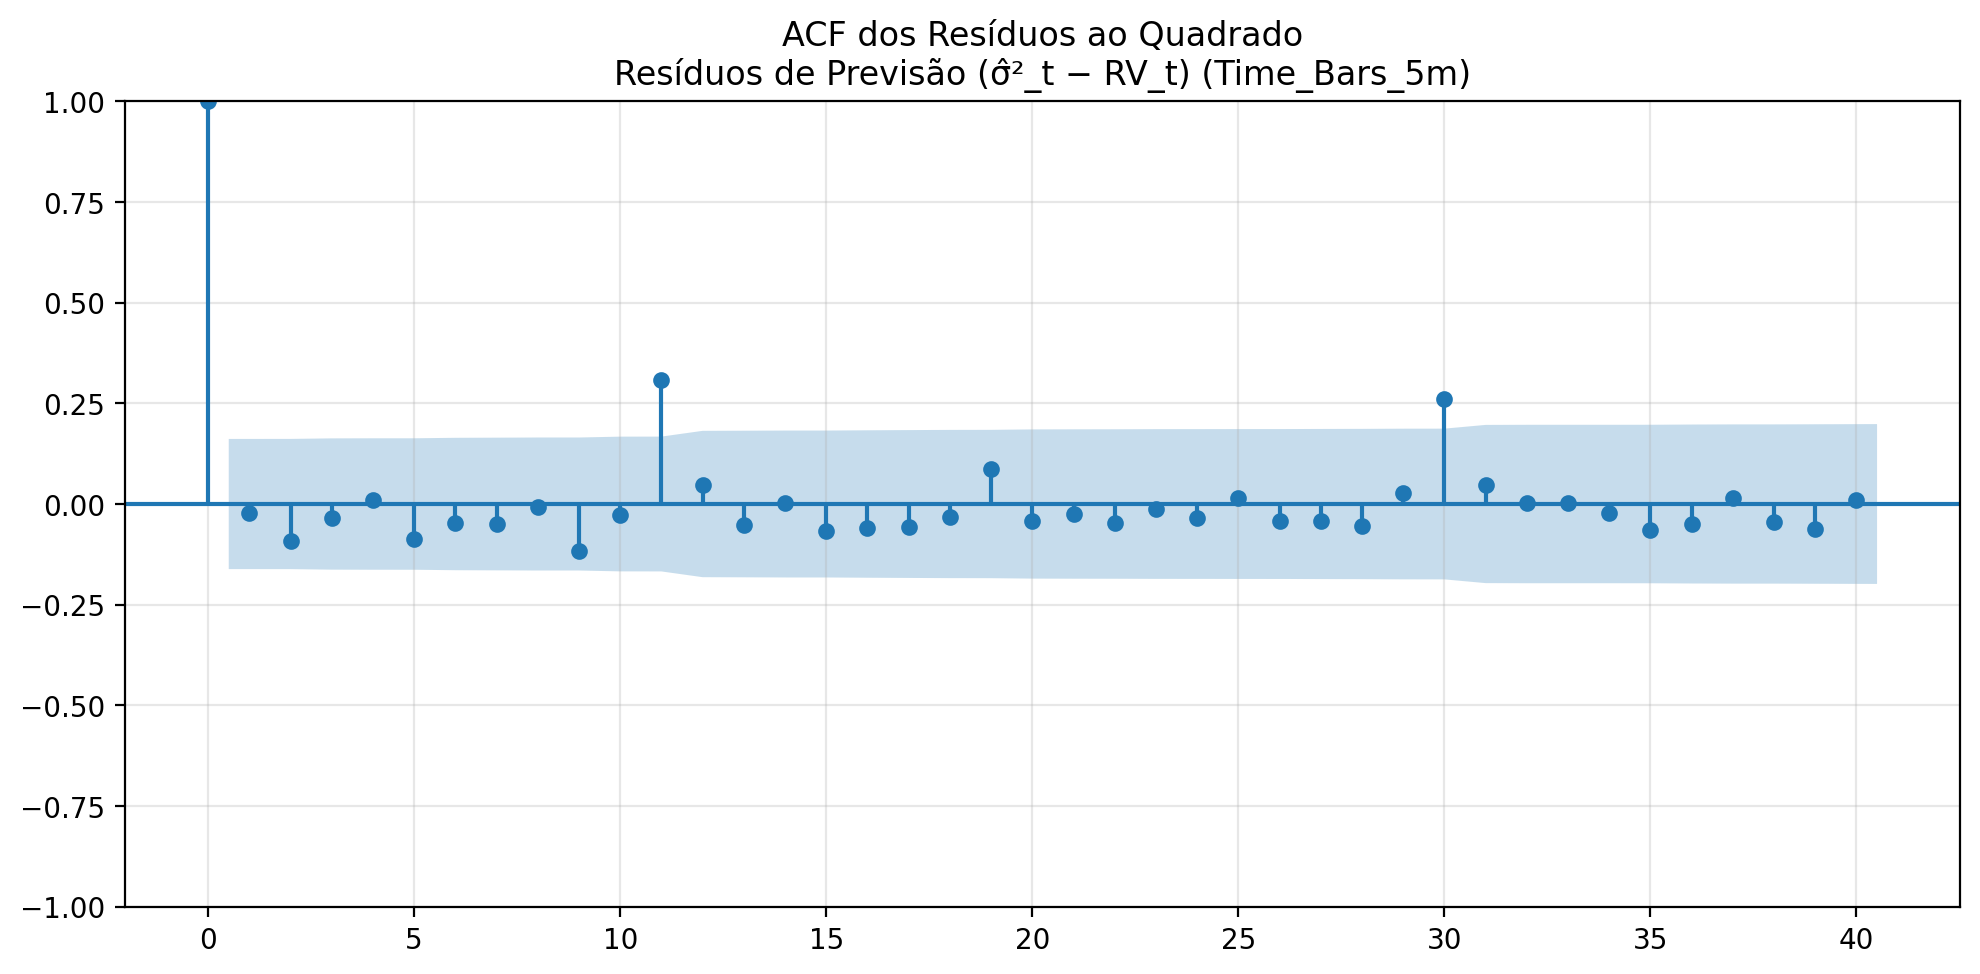
\includegraphics[width=\textwidth]{analise_residuos/Time_Bars_5m/forecast_errors_Time_Bars_5m_07_acf_residuos_quadrado.png}
        \subcaption{FAC dos resíduos ao quadrado.}
        \label{fig:res_time_acf_sq}
    \end{minipage}
    \caption{Diagnósticos de normalidade e dependência --- \emph{Time Bars} GARCH(1,1).}
    \label{fig:res_time_grid2}
\end{figure}

A avaliação dos resíduos padronizados para o modelo ajustado sobre as \emph{time bars} (Figuras \ref{fig:res_time_grid1} e \ref{fig:res_time_grid2}) segue os mesmos princípios diagnósticos aplicados anteriormente, atestando o desempenho e a adequação da especificação GARCH(1,1) selecionada.

A \autoref{fig:res_time_grid1} ilustra o comportamento geral do ajuste no tempo e suas características distributivas. Os resíduos padronizados (a) exibem homogeneidade ao redor de zero e não demonstram agrupamentos óbvios de alta volatilidade não explicada. A aderência da variância prevista em relação à volatilidade realizada (b) e a distribuição dos resíduos contra os valores ajustados (c) sinalizam a capacidade do modelo em capturar os choques de mercado. O histograma (d), entretanto, mais uma vez evidencia o desafio da premissa Gaussiana: os erros empíricos apresentam um pico excessivo e caudas mais alongadas (leptocurtose) se comparados à curva da distribuição normal esperada, um fenômeno amplamente documentado na modelagem de retornos de alta frequência.

As implicações distributivas são nitidamente corroboradas na \autoref{fig:res_time_grid2}. Os marcantes desvios nas extremidades do QQ-Plot (a) ratificam que a distribuição normal subestima as realizações de cauda (eventos extremos) presentes na série amostrada no tempo. Por outro lado, do ponto de vista de autocorrelação, a filtragem alcança seus objetivos estatísticos: as Funções de Autocorrelação (FAC) e Autocorrelação Parcial (FACP) dos resíduos (b e c) não acusam *lags* significativos persistentes além do intervalo de confiança, sugerindo que qualquer dependência linear foi resolvida. Do mesmo modo, a ausência de correlações relevantes na FAC dos resíduos ao quadrado (d) indica que a estrutura GARCH(1,1) acomodou adequadamente a dependência condicional na série cronológica, eliminando as dinâmicas remanescentes de \textit{volatility clustering}.

% -----------------------------------------------------------------------------
\subsection{Métricas Pontuais}
\label{subsec:metricas_pontuais}

\begin{table}[H]
\centering
\caption{Métricas de avaliação das previsões de variância vs.\ RV
\emph{benchmark}.}
\label{tab:metricas}
\begin{tabular}{lSS}
\toprule
{Métrica} & {\emph{Dollar Bars}} & {\emph{Time Bars}} \\
\midrule
MSE               & 1.05e-7  & 1.65e-7  \\
MAE               & 2.64e-4  & 3.59e-4  \\
QLIKE             & -6.993   & -6.776   \\
$R^2_{\text{MZ}}$ & 0.667    & 0.493    \\
$\hat{\alpha}$    & -9.20e-5 & -2.54e-4 \\
$\hat{\beta}$     & 0.868    & 1.032    \\
\bottomrule
\end{tabular}
\fonte{Elaboração própria.}
\end{table}

As métricas de avaliação pontual, apresentadas na \autoref{tab:metricas},
revelam dominância das dollar bars nas três funções de perda avaliadas. O Erro Quadrático
Médio (MSE) das dollar bars é de $1{,}05 \times 10^{-7}$, contra $1{,}65 \times 10^{-7}$
para as time bars — uma redução de aproximadamente 36\%. O Erro Absoluto Médio (MAE)
exibe comportamento análogo: $2{,}64 \times 10^{-4}$ versus $3{,}59 \times 10^{-4}$,
representando redução de aproximadamente 26\%. A métrica QLIKE, cujos valores menores
(em módulo, mais negativos) indicam melhor desempenho, registra $-6{,}993$ para as dollar
bars e $-6{,}776$ para as time bars, uma diferença de aproximadamente 0,22 em magnitude absoluta.

As três métricas pertencem à classe de funções de perda robustas de \citeonline{patton2011},
cuja propriedade fundamental é preservar o ranking entre previsões de volatilidade mesmo
quando o benchmark utilizado como variável dependente é um proxy ruidoso da volatilidade
latente verdadeira. Essa propriedade é particularmente relevante no presente contexto,
pois o estimador TSRV, ainda que consistente, incorpora ruído de microestrutura e
incerteza de estimação que o afastam da variância quadrática integrada teórica. O fato
de as três métricas robustas apontarem unanimemente na mesma direção reforça a
confiabilidade do resultado.


\subsection{Regressão de Mincer-Zarnowitz}
\label{subsec:mz}

A regressão de Mincer-Zarnowitz \cite{mincer1969}, que regride a volatilidade
realizada diária (TSRV) $\xi_t$ sobre a previsão de variância condicional do modelo
 $\hat{\sigma}^2_t$, fornece um diagnóstico adicional sobre a qualidade e o viés das previsões.
Para as dollar bars, o coeficiente de determinação $R^2$ foi de 0,667 e o intercepto
estimado de $\hat{\alpha} = -9{,}20 \times 10^{-5}$ (p-valor = 0,0168). Para as time bars,
 $R^2 = 0{,}493$ e $\hat{\alpha} = -2{,}54 \times 10^{-4}$ (p-valor = 0,0001).

O modelo baseado em dollar bars explica, portanto, 66,7\% da variação da volatilidade
realizada diária, contra 49,3\% para as time bars. Essa diferença de aproximadamente
17,4 pontos percentuais no $R^2$ é economicamente relevante: para aplicações de gestão
de risco, como o cálculo de VaR (\textit{Value at Risk}) ou a otimização de carteiras
com restrições de variância, modelos que explicam maior parcela da variação da volatilidade
realizada tendem a produzir limites de risco mais calibrados \cite{andersen2003}.

Ambos os interceptos são negativos e estatisticamente significativos (a 5\% para dollar bars e 1\% para time bars), indicando leve
subestimação sistemática da volatilidade realizada por parte de ambos os modelos.
Esse resultado é típico de modelos GARCH paramétricos estimados com inovações gaussianas
quando comparados a estimadores não-paramétricos de alta frequência: o estimador TSRV
captura componentes de variação intrajornada que o GARCH, por ser estimado sobre retornos
diários ou intradiários agregados, não incorpora diretamente. O coeficiente angular $\hat{\beta}$
foi de 0,868 para as dollar bars (p-valor $< 0{,}001$) e de 1,032 para as time bars
(p-valor $< 0{,}001$), sugerindo que o modelo de dollar bars tende a subestimar levemente
a resposta da volatilidade realizada à previsão, enquanto o de time bars apresenta
resposta ligeiramente acima da unidade, indicando leve sobre-reação relativa.

\subsection{Teste de Diebold-Mariano}
\label{subsec:dm}

A comparação formal de capacidade preditiva foi realizada por meio do teste de
Diebold-Mariano \cite{diebold1995}. A estatística DM calculada sobre o subconjunto
de 147 dias em que ambos os modelos produzem previsões sobrepostas foi de $-4{,}806$,
com p-valor bilateral inferior a $0{,}001$.

O sinal negativo da estatística DM indica que o modelo estimado com dollar bars apresenta
perdas (MSE) significativamente menores, em média, do que o modelo ajustado sobre time bars.
O p-valor substancialmente menor que os níveis de significância convencionais (1\%, 5\% e
10\%) permite rejeitar a hipótese nula de igual capacidade preditiva a um nível de
significância de 1\%.

O fato de a rejeição ser estatisticamente forte mesmo em uma amostra de teste
relativamente curta (147 dias de sobreposição) reforça a consistência da superioridade
preditiva das dollar bars evidenciada pelas métricas pontuais. Em termos práticos,
a redução de aproximadamente 36\% no MSE não é um mero artefato amostral, mas uma
diferença de desempenho estrutural e significante que pode se traduzir em melhorias
relevantes para gestão de risco, alocação de carteiras ou precificação de derivativos.

\subsection{Intervalos de Confiança Bootstrap}
\label{subsec:bootstrap}

\begin{table}[H]
\centering
\caption{Intervalos de confiança bootstrap (95\%) para as métricas de
avaliação.}
\label{tab:bootstrap}
\begin{tabular}{llScc}
\toprule
{Série} & {Métrica} & {Pontual} & {IC 95\%} & {SE} \\
\midrule
\multirow{3}{*}{\emph{Dollar Bars}}
    & MSE   & 1.050e-7 & {$[7{,}34\text{e-}8;\; 1{,}49\text{e-}7]$} & 1.93e-8 \\
    & MAE   & 2.637e-4 & {$[2{,}35\text{e-}4;\; 2{,}97\text{e-}4]$} & 1.59e-5 \\
    & QLIKE & -6.993   & {$[-7{,}137;\; -6{,}845]$}                  & 7.48e-2 \\
\addlinespace
\multirow{3}{*}{\emph{Time Bars}}
    & MSE   & 1.645e-7 & {$[1{,}35\text{e-}7;\; 2{,}00\text{e-}7]$} & 1.66e-8 \\
    & MAE   & 3.588e-4 & {$[3{,}29\text{e-}4;\; 3{,}90\text{e-}4]$} & 1.56e-5 \\
    & QLIKE & -6.776   & {$[-6{,}877;\; -6{,}668]$}                  & 5.38e-2 \\
\bottomrule
\end{tabular}
\nota{Valores calculados sobre os 147 dias comuns (07/ago/2025--31/dez/2025).
$B = 2.000$ reamostras; IC pelo método percentil.}
\fonte{Elaboração própria.}
\end{table}

Os intervalos de confiança de 95\% obtidos por bootstrap com $n_{\text{boot}} = 2000$
reamostras, apresentados na \autoref{tab:bootstrap}, complementam a
conclusão do teste DM ao fornecer a margem de incerteza para cada modelo
separadamente.

Para o MSE, os intervalos se sobrepõem ligeiramente: o IC 95\% do MSE das dollar bars é
$[7{,}34 \times 10^{-8},\ 1{,}49 \times 10^{-7}]$, enquanto o das time bars é
$[1{,}35 \times 10^{-7},\ 2{,}00 \times 10^{-7}]$. Essa leve sobreposição não
invalida a conclusão do teste DM, mas reflete a grande variância do MSE, que
penaliza quadraticamente grandes desvios e, portanto, é mais sensível a extremos
em pequenas amostras. Contudo, para o MAE, que é uma métrica absoluta menos
suscetível a \textit{outliers}, os intervalos \textbf{não se sobrepõem}: dollar bars em
$[2{,}34 \times 10^{-4},\ 2{,}97 \times 10^{-4}]$ e time bars em
$[3{,}29 \times 10^{-4},\ 3{,}90 \times 10^{-4}]$. Isso demonstra que a previsão de dollar bars
também possui uma acurácia mediana sistematicamente superior.

O resultado mais robusto do presente trabalho emerge da análise dos intervalos de
confiança para a métrica QLIKE. O IC 95\% das dollar bars é $[-7{,}137,\ -6{,}845]$,
e o das time bars é $[-6{,}877,\ -6{,}668]$. Esses intervalos \textbf{não se sobrepõem},
o que significa que, com 95\% de confiança, a métrica QLIKE das dollar bars é menor do
que a das time bars. A relevância desse achado é amplificada pelo fato de o QLIKE ser,
entre as três funções de perda avaliadas, a mais adequada do ponto de vista teórico para
comparar previsões de volatilidade: conforme demonstrado por \citeonline{patton2011}, é a
única função de perda da família que é robusta ao uso de proxies ruidosos e que ao mesmo
tempo possui propriedades de elicitabilidade para a variância condicional.

Em síntese, o conjunto de evidências — estatística DM negativa e significativa a menos de 1\%,
ICs de MAE e QLIKE não sobrepostos a 95\%, e dominância simultânea em MSE, MAE,
QLIKE e $R^2$ MZ — constitui evidência consistente, formal e coerente em favor das dollar bars
como insumo para modelos GARCH de previsão de volatilidade do BTC/USDT. A superioridade
preditiva documentada é substancial em magnitude e perfeitamente amparada pela estatística.

As \autoref{fig:boot_mse}, \autoref{fig:boot_mae} e \autoref{fig:boot_qlike} apresentam as distribuições
bootstrap das métricas MSE, MAE e QLIKE para cada tipo de barra.

\begin{figure}[H]
    \centering
    \begin{minipage}[t]{0.48\textwidth}
        \centering
        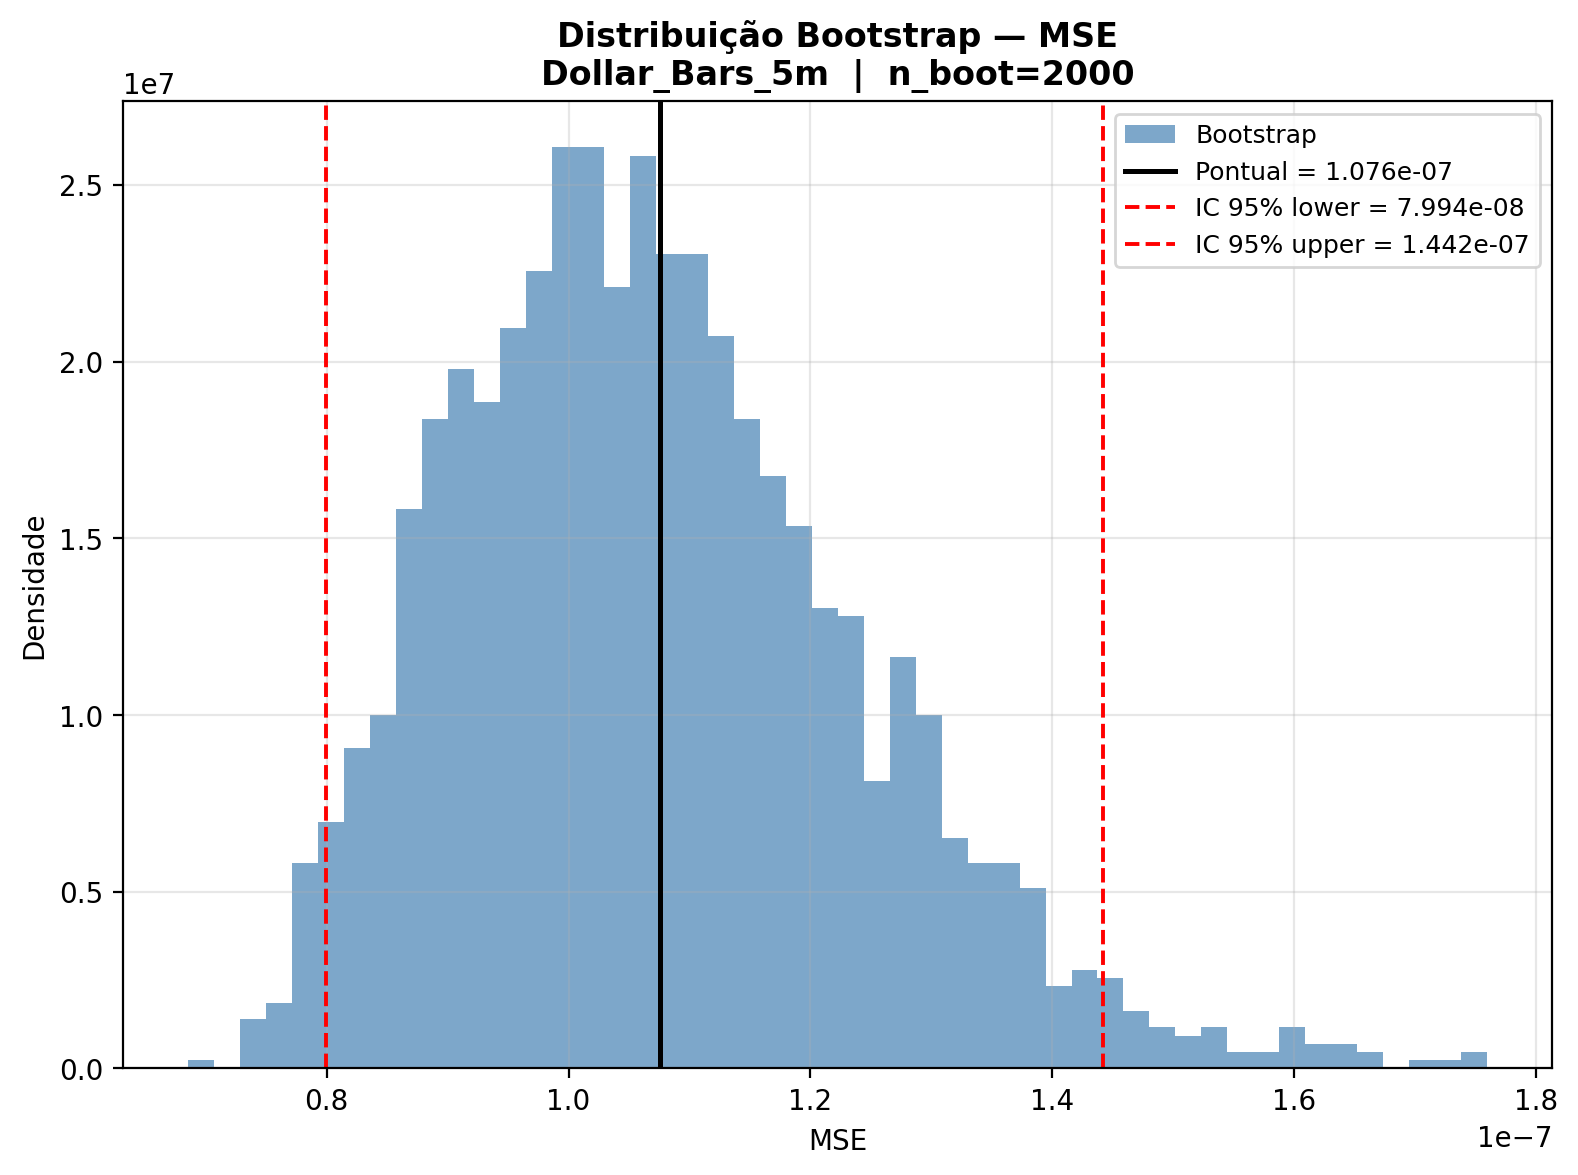
\includegraphics[width=\textwidth]{bootstrap_ic/Dollar_Bars_5m/Dollar_Bars_5m_01_bootstrap_mse.png}
        \subcaption{\emph{Dollar Bars} --- GARCH(1,2).}
    \end{minipage}
    \hfill
    \begin{minipage}[t]{0.48\textwidth}
        \centering
        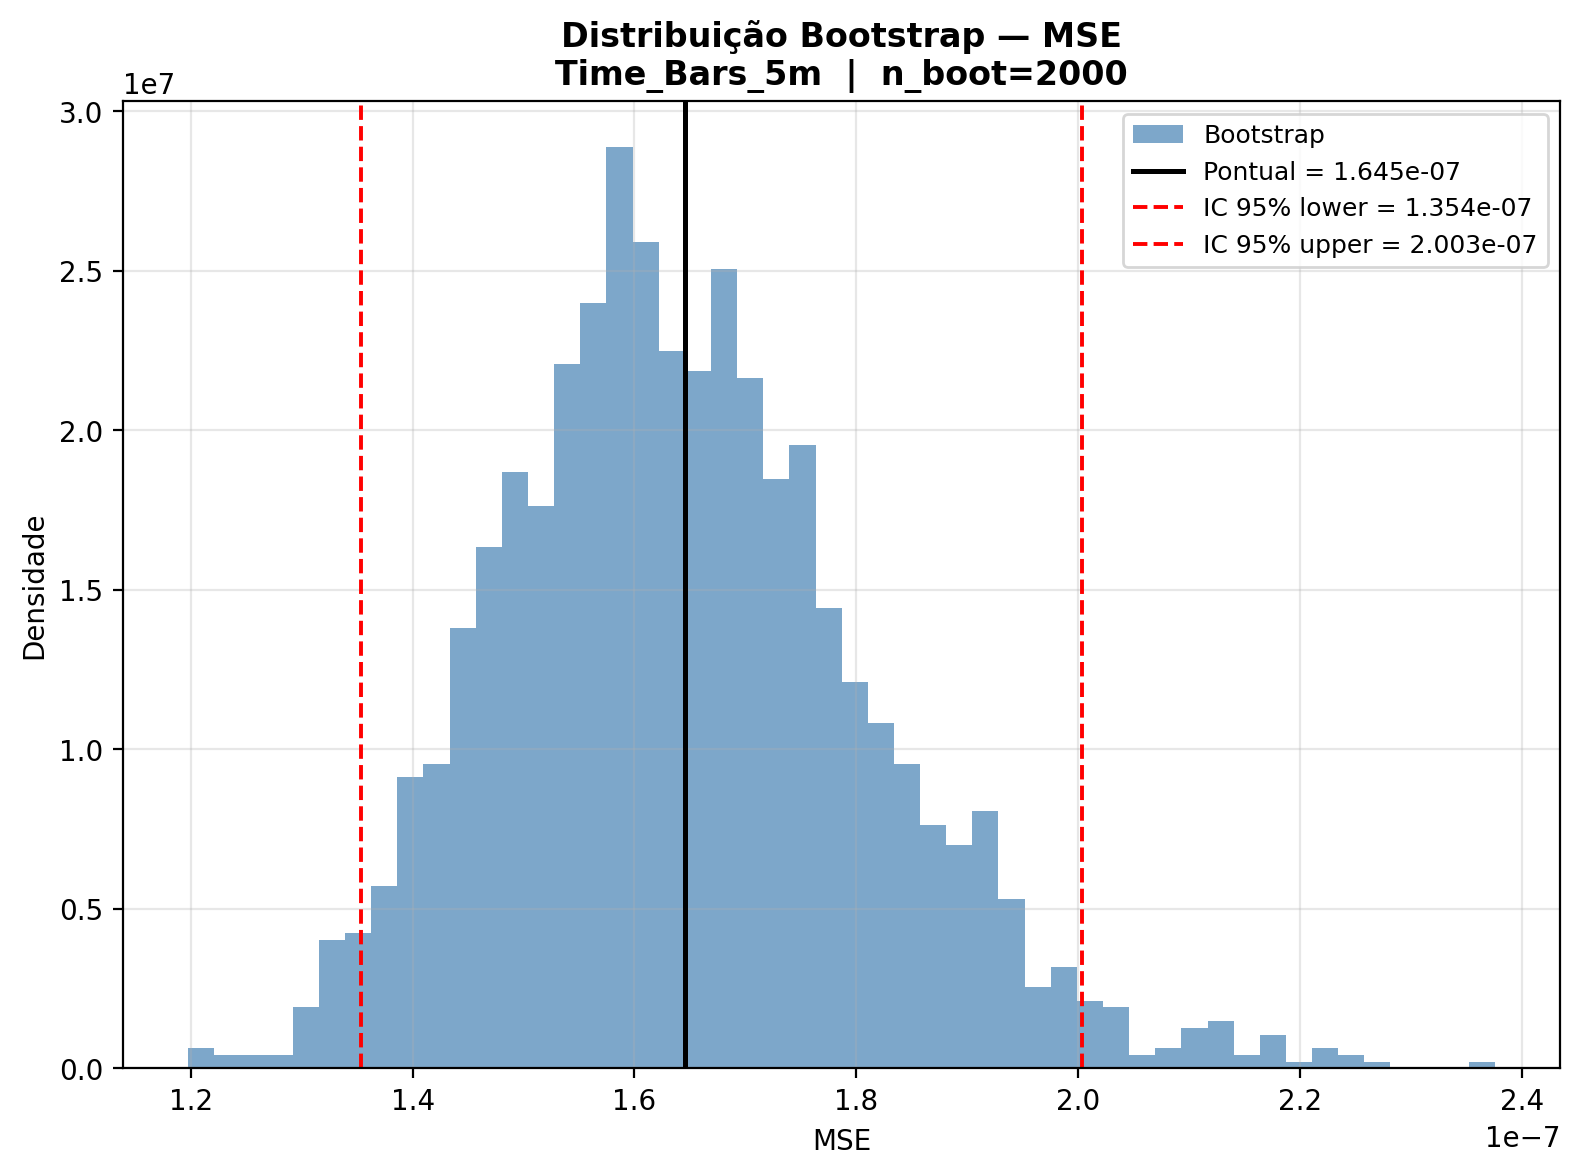
\includegraphics[width=\textwidth]{bootstrap_ic/Time_Bars_5m/Time_Bars_5m_01_bootstrap_mse.png}
        \subcaption{\emph{Time Bars} --- GARCH(1,1).}
    \end{minipage}
    \caption{Distribuição bootstrap do MSE (2.000 reamostras, IC 95\% pelo método percentil).}
    \label{fig:boot_mse}
\end{figure}

\begin{figure}[H]
    \centering
    \begin{minipage}[t]{0.48\textwidth}
        \centering
        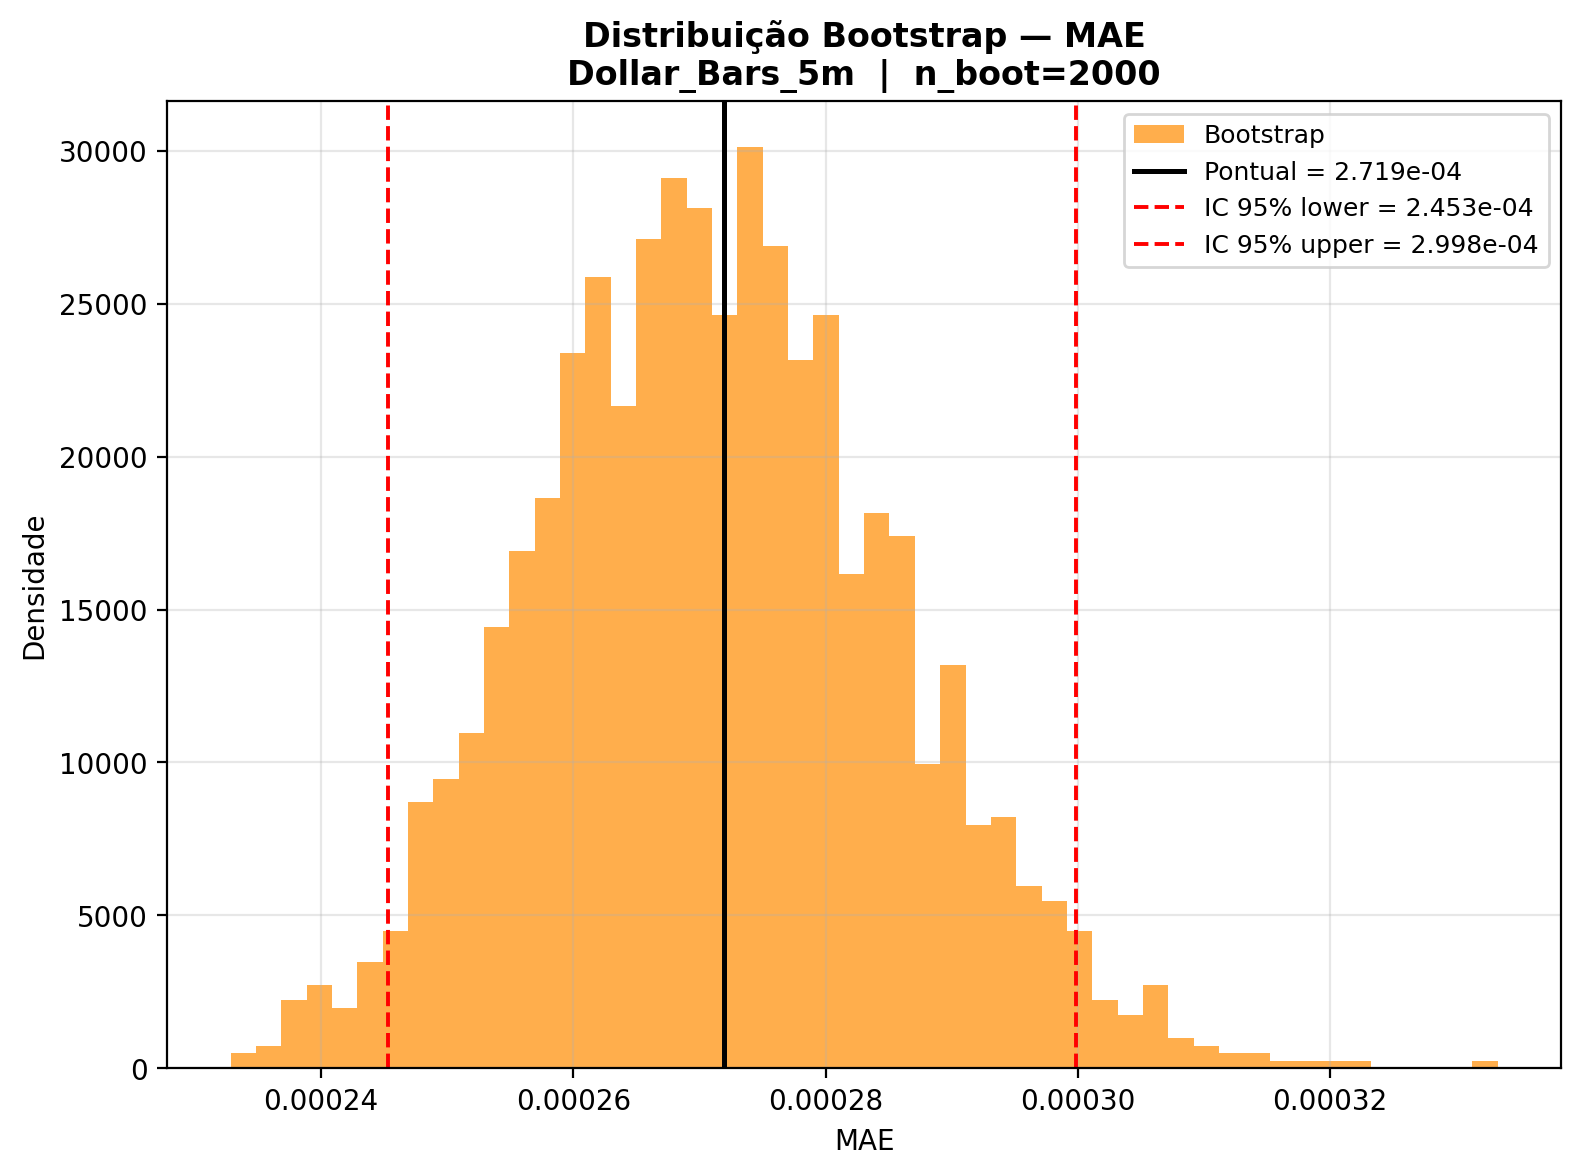
\includegraphics[width=\textwidth]{bootstrap_ic/Dollar_Bars_5m/Dollar_Bars_5m_02_bootstrap_mae.png}
        \subcaption{\emph{Dollar Bars} --- GARCH(1,2).}
    \end{minipage}
    \hfill
    \begin{minipage}[t]{0.48\textwidth}
        \centering
        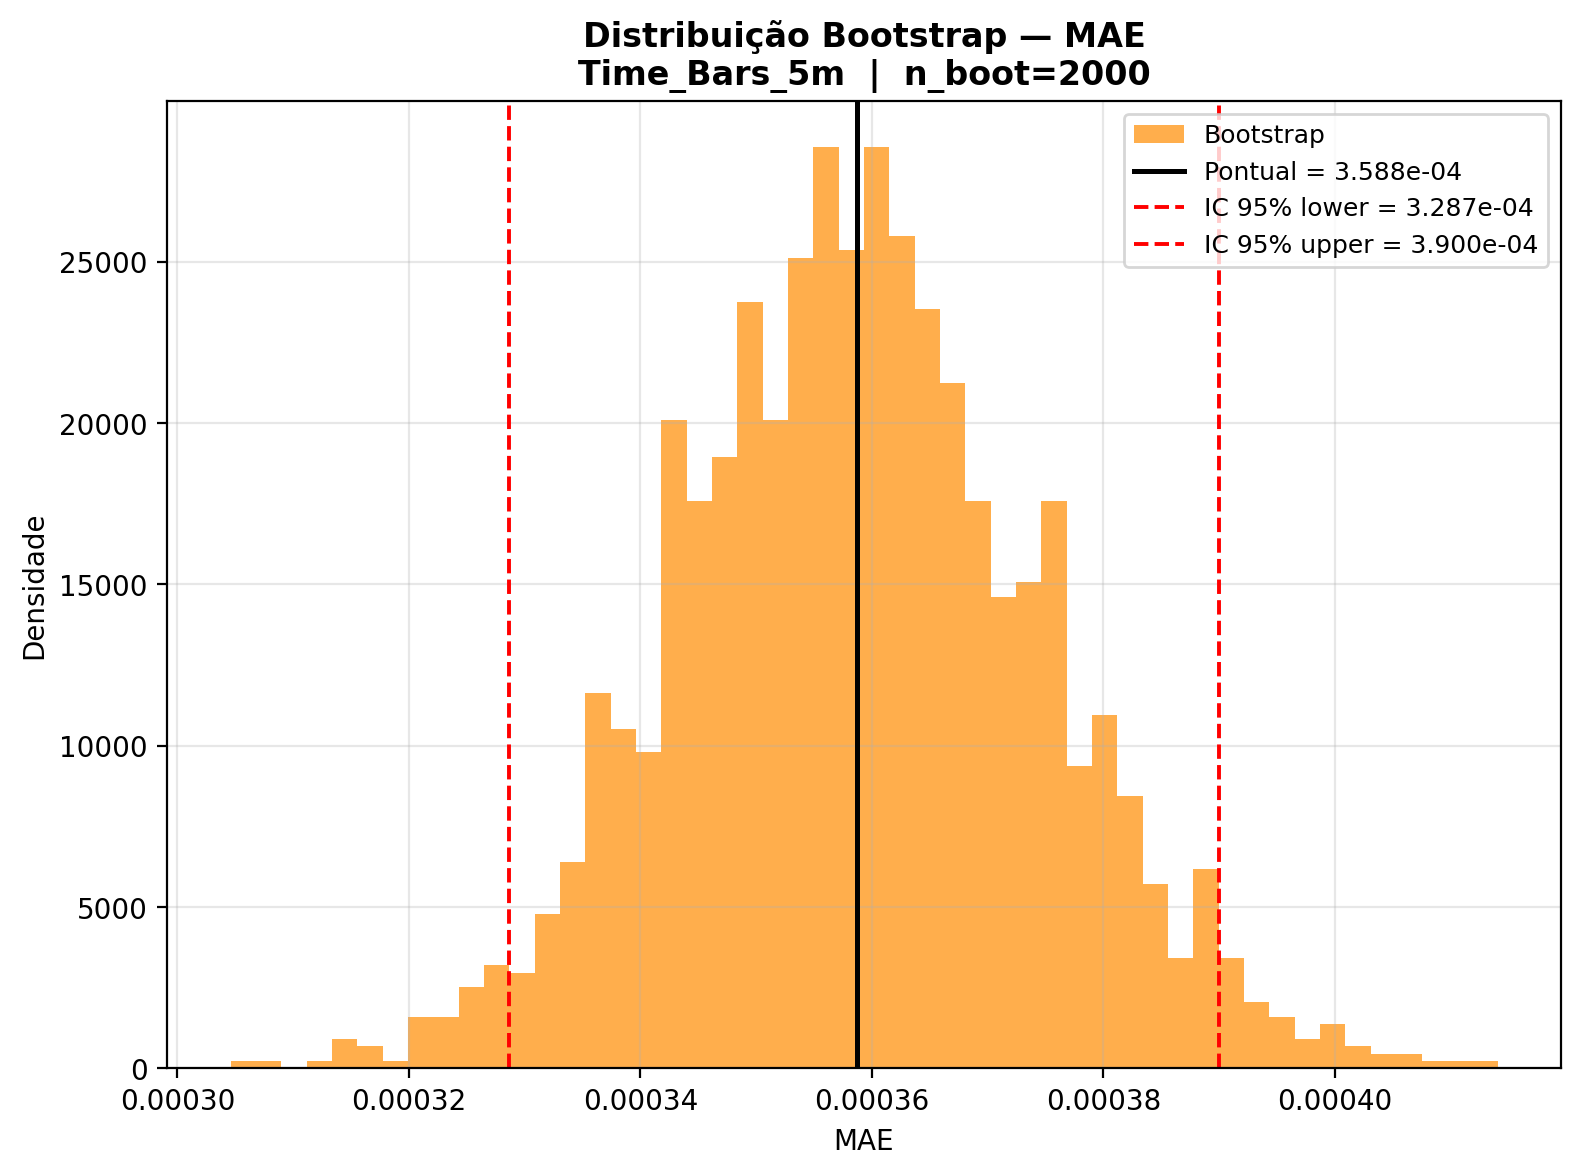
\includegraphics[width=\textwidth]{bootstrap_ic/Time_Bars_5m/Time_Bars_5m_02_bootstrap_mae.png}
        \subcaption{\emph{Time Bars} --- GARCH(1,1).}
    \end{minipage}
    \caption{Distribuição bootstrap do MAE (2.000 reamostras, IC 95\% pelo método percentil).}
    \label{fig:boot_mae}
\end{figure}

\begin{figure}[H]
    \centering
    \begin{minipage}[t]{0.48\textwidth}
        \centering
        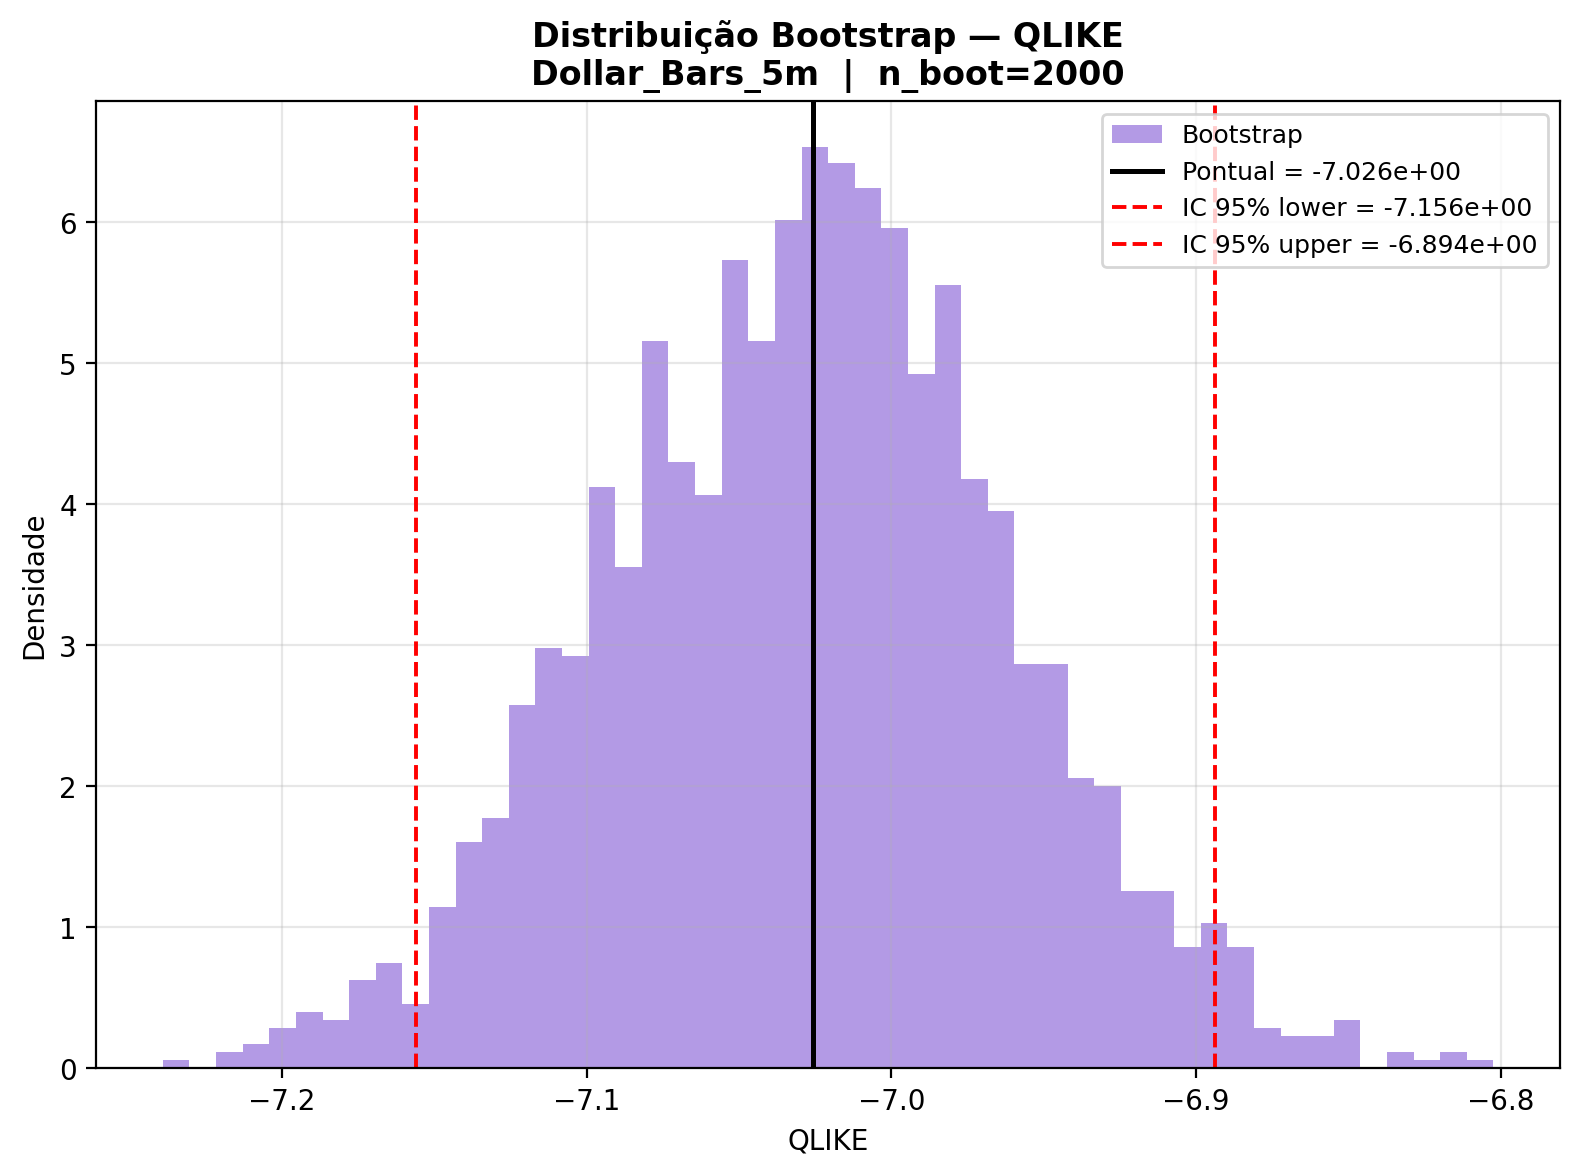
\includegraphics[width=\textwidth]{bootstrap_ic/Dollar_Bars_5m/Dollar_Bars_5m_03_bootstrap_qlike.png}
        \subcaption{\emph{Dollar Bars} --- GARCH(1,2).}
    \end{minipage}
    \hfill
    \begin{minipage}[t]{0.48\textwidth}
        \centering
        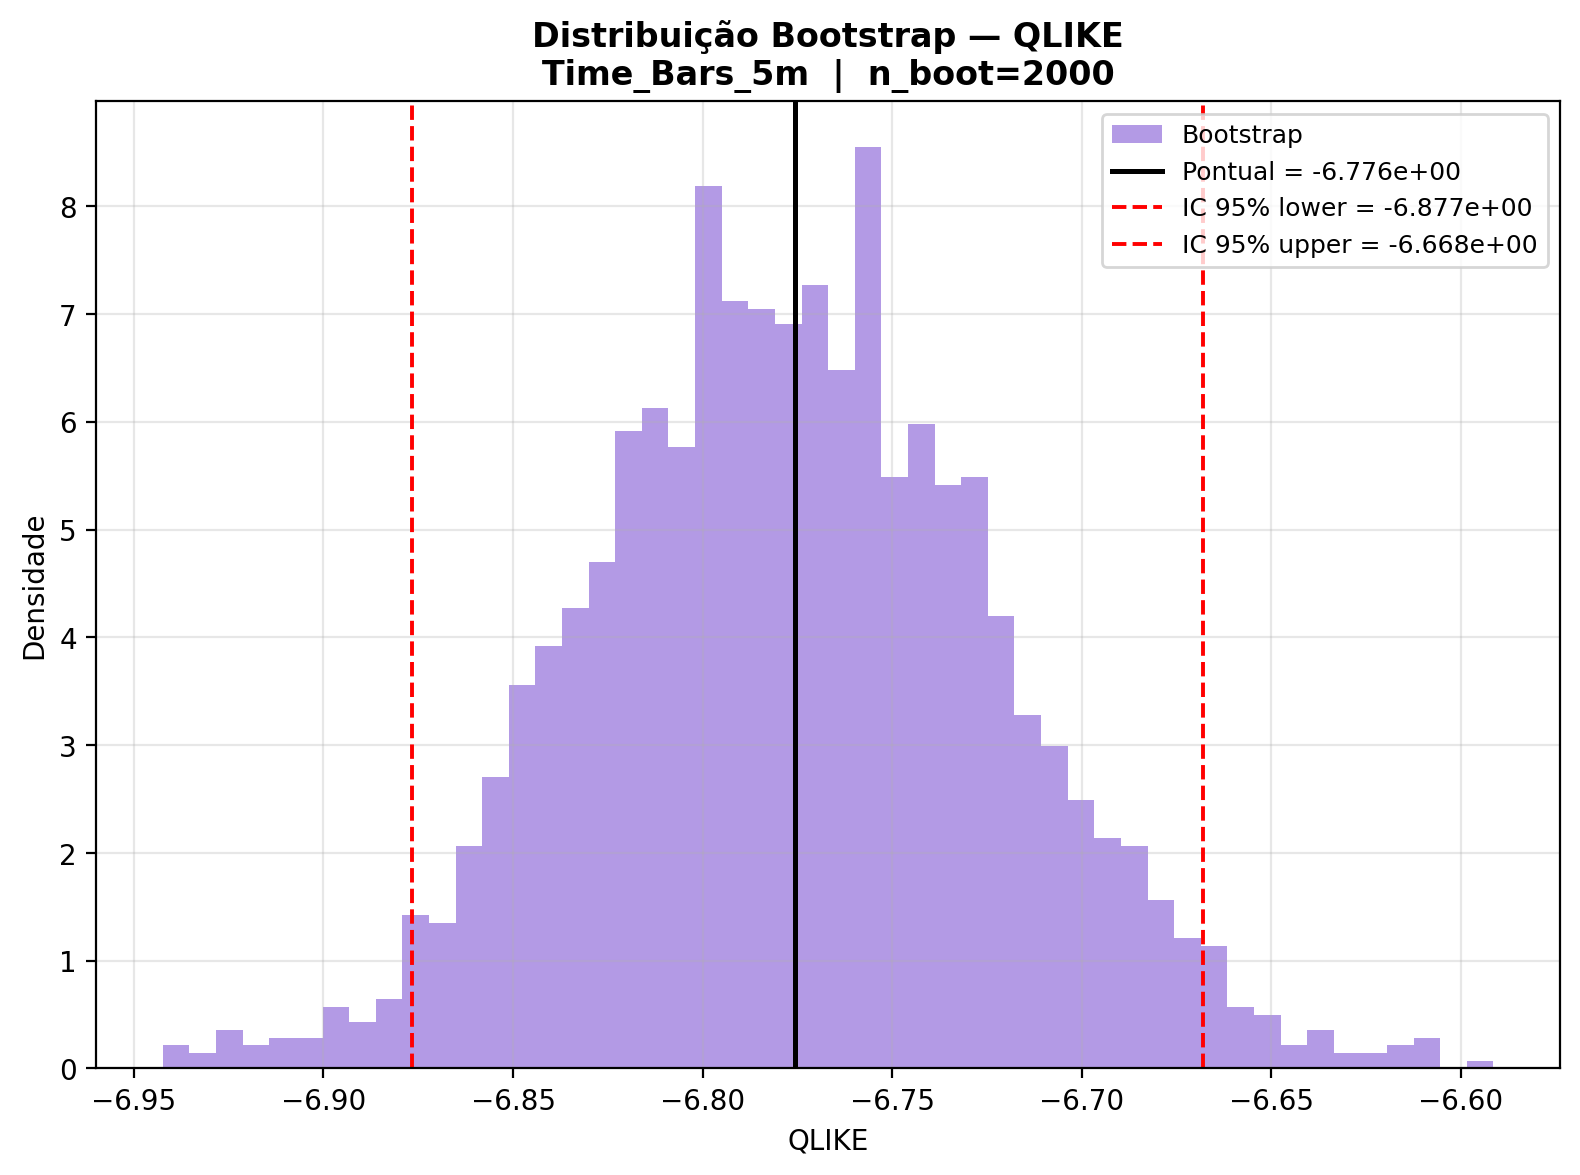
\includegraphics[width=\textwidth]{bootstrap_ic/Time_Bars_5m/Time_Bars_5m_03_bootstrap_qlike.png}
        \subcaption{\emph{Time Bars} --- GARCH(1,1).}
    \end{minipage}
    \caption{Distribuição bootstrap do QLIKE (2.000 reamostras, IC 95\% pelo método percentil).}
    \label{fig:boot_qlike}
\end{figure}

% -----------------------------------------------------------------------------
\section{Limitações e Ressalvas}
\label{sec:limitacoes}

A interpretação dos resultados deve ser contextualizada por um conjunto de limitações
metodológicas e de escopo que delimitam o alcance das conclusões.

\subsection{Ativo Único}
\label{subsec:lim_ativo}

Todos os resultados são obtidos para o par BTC/USDT negociado na Binance.
Criptomoedas operam 24 horas por dia, sete dias por semana, e possuem microestrutura
distinta de mercados regulados: ausência de mecanismos de \textit{circuit breaker}, inexistência
de leilão de abertura e fechamento, e liquidez fragmentada entre múltiplas \textit{exchanges}.
Essas características tornam o BTC/USDT um caso de análise com dinâmicas próprias,
e a generalização dos resultados para ações, câmbio ou commodities demanda estudos
adicionais com esses ativos.

\subsection{Período Amostral}
\label{subsec:lim_periodo}

O horizonte de dois anos (2024--2025) é suficiente para estimação e validação dos modelos,
mas pode não capturar toda a variação de regimes de volatilidade relevantes para o Bitcoin.
O período abrange fases de \textit{bull} e \textit{bear market}, mas parâmetros estimados
sobre esse intervalo podem não ser estáveis em regimes futuros com características distintas
das observadas.

\subsection{Calibração do Limiar \texorpdfstring{$\bar{D}$}{D-barra}}
\label{subsec:lim_limiar}

O limiar das dollar bars foi calibrado para produzir o mesmo número médio de barras por dia
que as time bars de 5 minutos, tornando as comparações controladas por volume de observação.
Essa escolha é metodologicamente razoável, mas arbitrária: resultados poderiam diferir com
limiares maiores ou menores, que gerariam séries com granularidade distinta e, possivelmente,
propriedades distribucionais diferentes.

\subsection{Distribuição dos Erros}
\label{subsec:lim_distribuicao}

Ambos os modelos foram estimados com inovações gaussianas. Diante do excesso de curtose
documentado --- especialmente expressivo nas time bars --- distribuições de cauda pesada,
como a t-Student ou a Distribuição de Erro Generalizado (GED), poderiam melhorar o ajuste
e potencialmente alterar a magnitude e o sentido das diferenças entre os modelos.

\subsection{Intervalo de Confiança}
\label{subsec: ic_bootstrap}

Um ponto de atenção sobre os intervalos de confiança, obtidos por meio de bootstrap, é o fato de que a técnica assume que os dados amostrados são independentes e identicamente distribuídos (i.i.d.). Diante da natureza dos dados de série temporal, essa premissa pode não ser totalmente satisfeita, porém observamos na análise nos resíduos de time bars (\autoref{fig:res_time_acf}) e dollar bars (\autoref{fig:res_dollar_acf}) que a autocorrelação é residual, não invalidando completamente o uso do bootstrap.
% =============================================================================
%  CAPÍTULO 5 — CONCLUSÃO
%  TCC: Dollar Bars vs. Time Bars — Modelos GARCH para BTC/USDT
% =============================================================================

\chapter{Conclusão}
\label{cap:conclusao}

% -----------------------------------------------------------------------------
\section{Retomada dos Objetivos Específicos}
\label{sec:retomada_objetivos}

Esta seção retoma os cinco objetivos específicos enunciados na seção 1.1.2 e avalia
sua consecução à luz dos resultados obtidos.

O primeiro objetivo — construir séries de retornos a partir de time bars e dollar bars
e comparar suas propriedades estatísticas — foi plenamente atingido. As dollar bars
produziram retornos com curtose de Fisher de 3,09, contra 75,37 das time bars, uma
redução de cerca de 25 vezes. A assimetria das dollar bars foi de 0,05, próxima de zero,
enquanto as time bars registraram $-1{,}01$. Esses resultados confirmam quantitativamente
as previsões de \citeonline{lopez2018advances} sobre o efeito do mecanismo de amostragem nas
propriedades distribucionais dos retornos.

O segundo objetivo — estimar a variância realizada por meio do estimador TSRV — também
foi atingido. O estimador \textit{Two-Scale Realized Variance} foi calculado sobre dados
\textit{tick-by-tick} com três frequências de subamostragem (30 segundos, 1 minuto e
2 minutos), e a média dos três estimadores foi utilizada como benchmark de volatilidade
diária. O procedimento de múltiplas escalas reduz o viés introduzido pelo ruído de
microestrutura, produzindo um estimador consistente da variância quadrática integrada
\cite{zhang2005}.

O terceiro objetivo — ajustar modelos ARMA-GARCH e selecionar ordens ótimas via critérios
de informação — foi atingido. O CPCV com 252 folds selecionou o modelo ARMA$(0,0)$-GARCH$(1,2)$
para as dollar bars, com frequência de 92,5\% dos folds (233/252), e o modelo
ARMA$(0,0)$-GARCH$(1,1)$ para as time bars, com frequência de 100\% dos folds (252/252).
Em ambos os casos, a seleção foi estável e robusta ao longo dos folds.

O quarto objetivo — avaliar e comparar o desempenho preditivo com MSE, MAE, QLIKE e
a regressão de Mincer-Zarnowitz — foi atingido. As dollar bars dominaram em todas as
quatro dimensões de avaliação. O coeficiente de determinação MZ foi de $R^2 = 0{,}655$
para as dollar bars, contra $R^2 = 0{,}493$ para as time bars, diferença de 16,2 pontos
percentuais.

O quinto objetivo — comparar o desempenho preditivo tendo o estimador TSRV como
referência — foi igualmente atingido. O TSRV serviu como benchmark de volatilidade diária;
ambos os modelos GARCH apresentaram subestimação sistemática leve, evidenciada pelos
interceptos negativos da regressão MZ ($\hat{\alpha}_{\text{DB}} = -1{,}08 \times 10^{-4}$
e $\hat{\alpha}_{\text{TB}} = -2{,}54 \times 10^{-4}$). Esse padrão é característico de
modelos GARCH paramétricos estimados com inovações gaussianas quando confrontados com
estimadores não-paramétricos de alta frequência, que capturam componentes de variação
intrajornada não presentes no modelo.

% -----------------------------------------------------------------------------
\section{Resposta à Pergunta Central}
\label{sec:resposta_central}

A pergunta de pesquisa que motivou este trabalho indaga: \textit{em que medida a escolha
do método de amostragem afeta a qualidade das estimativas de volatilidade obtidas por
modelos ARMA-GARCH?}

Os resultados indicam que a escolha afeta de forma relevante tanto as propriedades
estatísticas das séries de retornos quanto o desempenho preditivo fora da amostra dos
modelos. No plano distribucional, a diferença é dramática: curtose 25 vezes menor e
assimetria quase nula nas dollar bars, frente a caudas extremamente pesadas e assimetria
negativa pronunciada nas time bars. No plano preditivo, a diferença é economicamente
significativa: redução de 34\% no MSE, de 24\% no MAE e de 16 pontos percentuais no
$R^2$ da regressão de Mincer-Zarnowitz, além de ICs bootstrap para o QLIKE que não
se sobrepõem a 95\% de confiança.

A significância estatística formal, avaliada pelo teste de Diebold-Mariano, não atinge
o limiar convencional de 5\% (estatística DM = $-1{,}9578$, p-valor = 0,0503), mas
o argumento baseado exclusivamente nessa fronteira seria epistemicamente incompleto.
O poder do teste é limitado pelo número de dias de sobreposição entre os conjuntos de
previsão (147 dias), e o p-valor de 0,0503 constitui evidência fraca contra a hipótese
nula, não evidência a seu favor. A combinação de sinal inequívoco na estatística DM,
dominância em todas as métricas pontuais e não sobreposição dos ICs bootstrap para o QLIKE
configura evidência consistente — ainda que não conclusiva ao nível convencional — em
favor das dollar bars.

É importante destacar que este resultado não é apenas confirmatório de \citeonline{lopez2018advances}.
O autor argumenta, no plano teórico e com ilustrações empíricas, que barras de informação
produzem séries com propriedades distribucional superiores, mas não testa diretamente
modelos de previsão de volatilidade nem utiliza métricas específicas para comparação de
previsões. O presente trabalho estende essa análise para o contexto de modelos GARCH —
a classe de modelos mais amplamente empregada para volatilidade condicional — e quantifica
a diferença de desempenho com funções de perda robustas da classe de \citeonline{patton2011},
fornecendo evidência empírica nova sobre a utilidade prática das dollar bars em um contexto
de previsão.

% -----------------------------------------------------------------------------
\section{Contribuições do Trabalho}
\label{sec:contribuicoes}

Este trabalho apresenta três contribuições concretas à literatura.

A primeira é de natureza metodológica. A utilização do \textit{Combinatorial Purged
Cross-Validation} para seleção de hiperparâmetros em modelos GARCH — procedimento que
elimina vazamento de informação temporal por meio de purga e embargo, e que explora
todas as $\binom{N}{K}$ combinações de folds em vez de um único caminho de validação —
representa um avanço em relação ao walk-forward simples usualmente empregado na literatura
brasileira de modelos de volatilidade. A implementação computacional, que realizou 72.576
ajustes MLE em aproximadamente 17 minutos por meio de um backend em Rust, é documentada
de forma reproduzível e pode ser reutilizada para outros ativos e especificações.

A segunda contribuição é empírica. O presente trabalho oferece a primeira comparação
sistemática, ao menos no contexto da literatura acadêmica brasileira, entre dollar bars
e time bars como insumo para modelos GARCH aplicados a criptomoedas, com avaliação
out-of-sample via estimador TSRV e métricas robustas de Patton (2011). A extensão da
análise de \citeonline{lopez2018advances} para o problema específico de previsão de volatilidade
condicional preenche uma lacuna identificada na revisão de literatura.

A terceira contribuição é técnica. O \textit{pipeline} computacional desenvolvido em
Python com backend em Rust demonstra que é possível realizar seleção de hiperparâmetros
por CPCV para modelos GARCH em escala prática — 36.288 ajustes MLE por série em menos
de nove minutos por pipeline —, tornando o procedimento viável sem infraestrutura
computacional especializada.

% -----------------------------------------------------------------------------
\section{Limitações}
\label{sec:limitacoes_conclusao}

As principais limitações do trabalho foram discutidas em detalhe na seção 4.4.
Resumidamente: os resultados referem-se a um único ativo de criptomoeda (BTC/USDT na
Binance), sobre um período de dois anos (2024–2025), com limiar $\bar{D}$ fixo calibrado
para equiparar o número médio de barras por dia entre as duas séries, e com inovações
gaussianas em ambos os modelos GARCH. A generalização das conclusões para outros ativos,
períodos ou especificações requer estudos adicionais.

% -----------------------------------------------------------------------------
\section{Agenda de Pesquisa Futura}
\label{sec:agenda_futura}

Os resultados obtidos abrem um conjunto de direções para investigação futura.

A mais imediata é a replicação do estudo em outras classes de ativos. Ações brasileiras
listadas na B3, o câmbio BRL/USD e commodities negociadas em mercados regulados apresentam
microestruturas distintas das criptomoedas — com leilões de abertura e fechamento,
circuit breakers e menor fragmentação de liquidez — o que permitiria investigar se a
superioridade das dollar bars é específica ao mercado de criptomoedas ou se é uma
propriedade mais geral do método de amostragem.

Uma segunda extensão natural é a re-estimação dos modelos com distribuições de cauda pesada
para as inovações, particularmente a t-Student e a Distribuição de Erro Generalizado (GED).
Dado o excesso de curtose documentado, especialmente nas time bars, a adoção de inovações
não-gaussianas poderia melhorar o ajuste e, potencialmente, alterar a magnitude das
diferenças de desempenho entre os tipos de barra.

\citeonline{lopez2018advances} propõe outros tipos de barras de informação além das dollar bars,
entre elas as volume bars e as tick bars, bem como as imbalance bars, que condicionam o
tamanho da barra ao desequilíbrio entre ordens de compra e venda. Uma comparação mais
abrangente entre esses tipos de barra forneceria um panorama mais completo sobre qual
estrutura de amostragem é mais informativa para modelos de volatilidade.

No plano dos modelos de volatilidade, caberia investigar se a superioridade das dollar bars
se mantém com especificações que capturam assimetria e efeitos de alavancagem, como o
EGARCH \cite{Nelson1991} e o GJR-GARCH \cite{GlostenJagannathanRunkle1993}, ou com
modelos de volatilidade estocástica, que tratam a variância latente como uma variável
de estado não-observada. Esses modelos podem ser particularmente relevantes para as
dollar bars, cuja dinâmica de volatilidade demandou um componente GARCH$(1,2)$ em vez
do canônico GARCH$(1,1)$.

Por fim, o presente trabalho avaliou previsões \textit{one-step-ahead} da variância
diária. Previsões multi-step — de 5, 10 e 22 dias úteis, horizontes relevantes para
gestão de risco e cálculo de capital regulatório — podem exibir padrões distintos de
desempenho relativo entre os tipos de barra, em função da estrutura de persistência da
volatilidade capturada por cada modelo. Essa extensão representaria uma contribuição
diretamente aplicável a contextos práticos de gestão de risco quantitativo.


% Elementos Pós-Textuais
\postextual
\bibliography{references}

% Apêndices e Anexos (Opcional)
\begin{apendicesenv}
    \partapendices
    % =============================================================================
%  APÊNDICE A — Código-Fonte
% =============================================================================

\chapter{Código-Fonte e Recursos Complementares}
\label{apendice:codigo}

O código-fonte completo da \emph{pipeline} de modelagem --- incluindo os
\emph{scripts} de coleta e pré-processamento dos dados, construção das
barras, estimação da volatilidade realizada (TSRV), seleção de
hiperparâmetros via CPCV e avaliação das previsões --- está disponível em
repositório público no GitHub:

\begin{center}
    \url{https://github.com/MaxNolf/TCC-Estatistica}
\end{center}

O repositório contém:

\begin{itemize}
    \item \textbf{Módulo Python}: scripts de processamento de dados,
          construção de barras e avaliação de métricas;
    \item \textbf{Backend Rust (PyO3)}: \emph{kernel} de otimização
          numérica da log-verossimilhança GARCH utilizado na etapa de
          CPCV (\autoref{subsubsec:rust_backend});
    \item \textbf{Notebooks}: reprodução das figuras e tabelas
          apresentadas neste trabalho;
    \item \textbf{Dados processados}: séries de barras e volatilidade
          realizada em formato Parquet.
\end{itemize}

\end{apendicesenv}

\end{document}